%# -*- coding: utf-8-unix -*-
%%==================================================
%% thesis.tex
%%==================================================

% 双面打印
\documentclass[master, fontset=adobe, openright, twoside, zihao=-4,submit]{sjtuthesis}
% \documentclass[bachelor, fontset=adobe, openany, oneside, zihao=-4, submit]{sjtuthesis} 
% \documentclass[master, fontset=adobe, zihao=-4, review]{sjtuthesis} 
% \documentclass[%
%   bachelor|master|doctor,	% 必选项
%   fontset=adobe|windows,  	% 只测试了adobe
%   oneside|twoside,		% 单面打印,双面打印(奇偶页交换页边距,默认)
%   openany|openright, 		% 可以在奇数或者偶数页开新章|只在奇数页开新章(默认)
%   zihao=-4|5,, 		% 正文字号:小四、五号(默认)
%   review,	 		% 盲审论文,隐去作者姓名、学号、导师姓名、致谢、发表论文和参与的项目
%   submit			% 定稿提交的论文,插入签名扫描版的原创性声明、授权声明 
% ]

% 逐个导入参考文献数据库
\addbibresource{bib/thesis.bib}
% \addbibresource{bib/chap2.bib}

\begin{document}

%% 无编号内容:中英文论文封面、授权页
%# -*- coding: utf-8-unix -*-
\title{基于眼动数据的立体图像质量评价}
\author{马宝岩}
\advisor{周军}
% \coadvisor{某某教授}
\defenddate{2016年1月8日}
\school{上海交通大学}
\institute{电子信息与电气工程学院}
\studentnumber{1130349147}
\major{电子与通信工程}

\englishtitle{Stereoscopic Image Quality Assessment Based on Eyetracking Data}
\englishauthor{\textsc{Ma Baoyan}}
\englishadvisor{Prof. \textsc{Zhou Jun}}
 %\englishcoadvisor{Prof. \textsc{Zhou Jun}}
\englishschool{Shanghai Jiao Tong University}
\englishinstitute{\textsc{School of Electronics and Communication Engineering} \\
  \textsc{Shanghai Jiao Tong University} \\
  \textsc{Shanghai, P.R.China}}
\englishmajor{Electronics and Communication Engineering}
\englishdate{Jan. 8th, 2016}


\maketitle

\makeenglishtitle

\makeatletter
\ifsjtu@submit\relax
	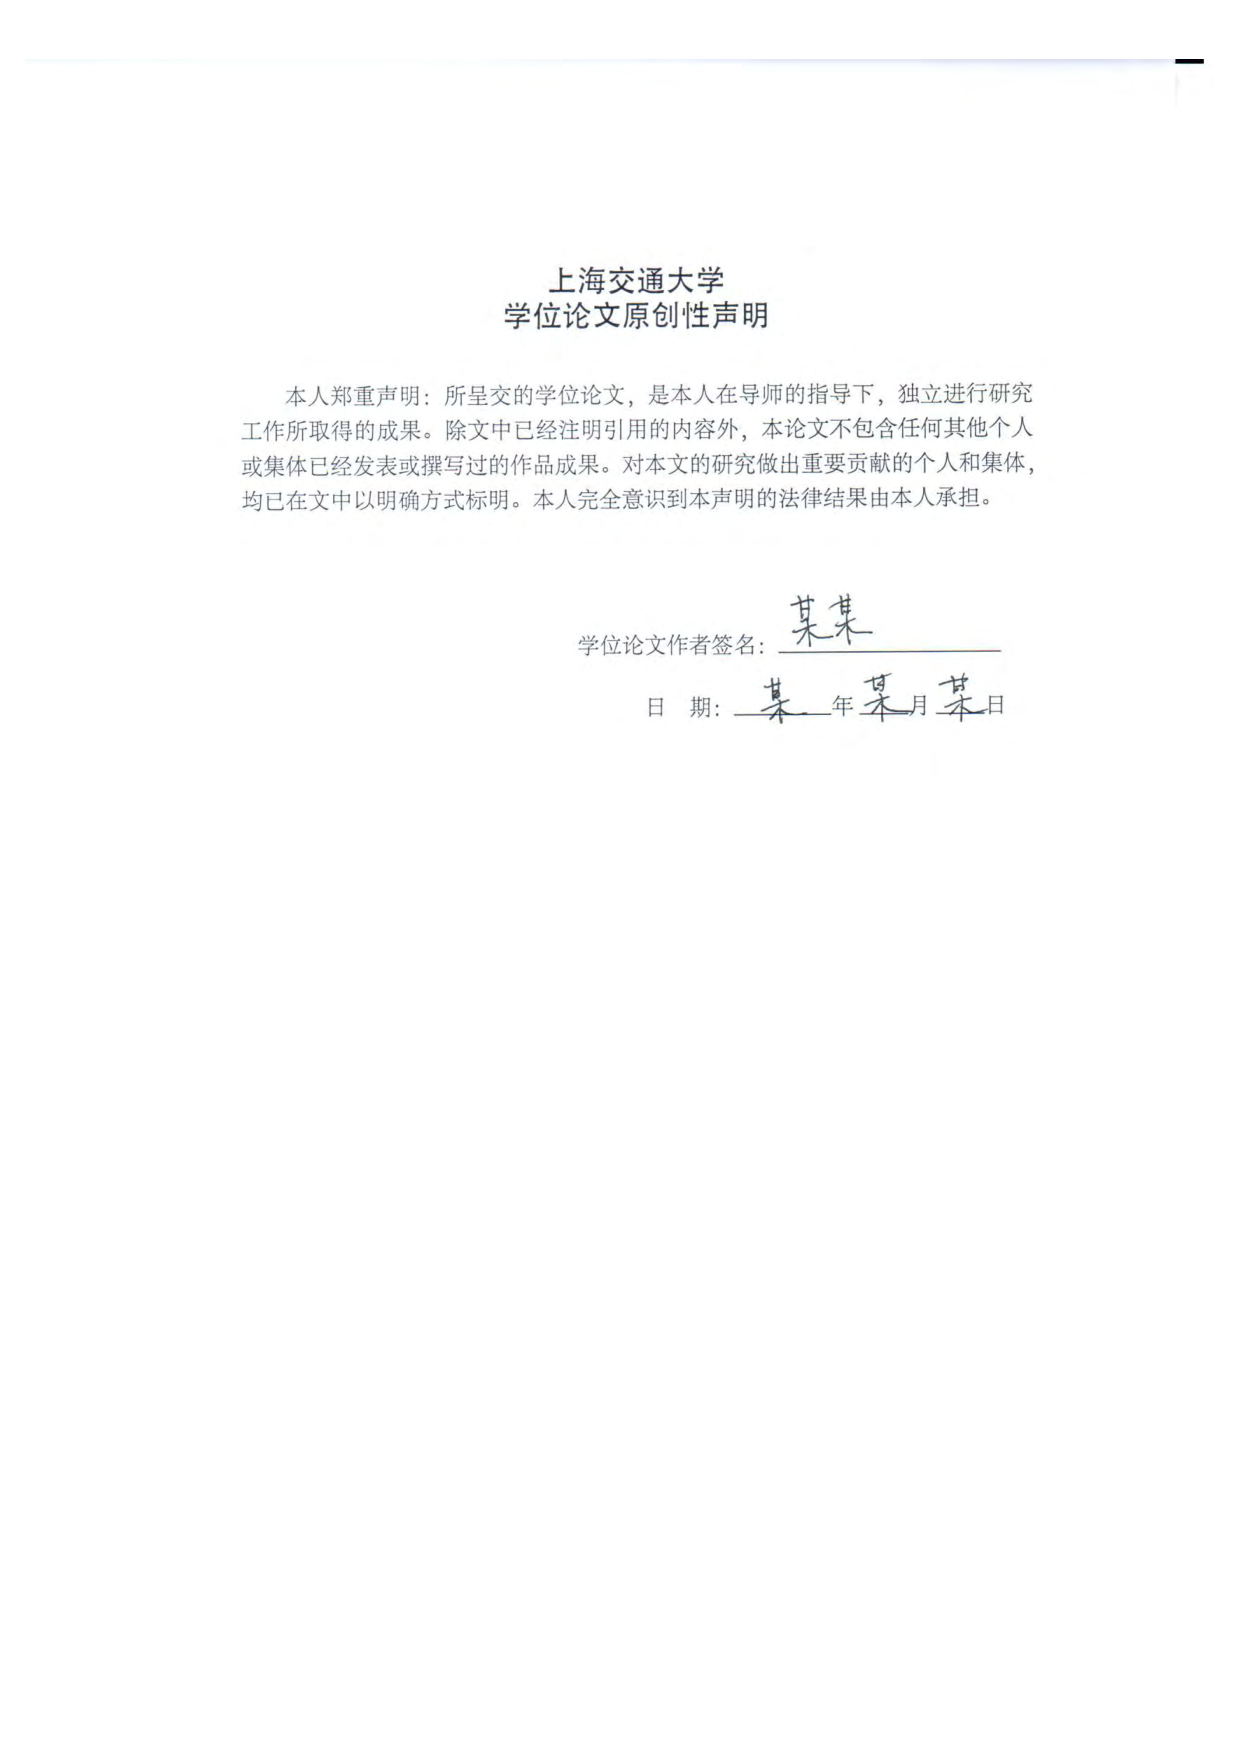
\includepdf{pdf/original.pdf}
	\cleardoublepage
	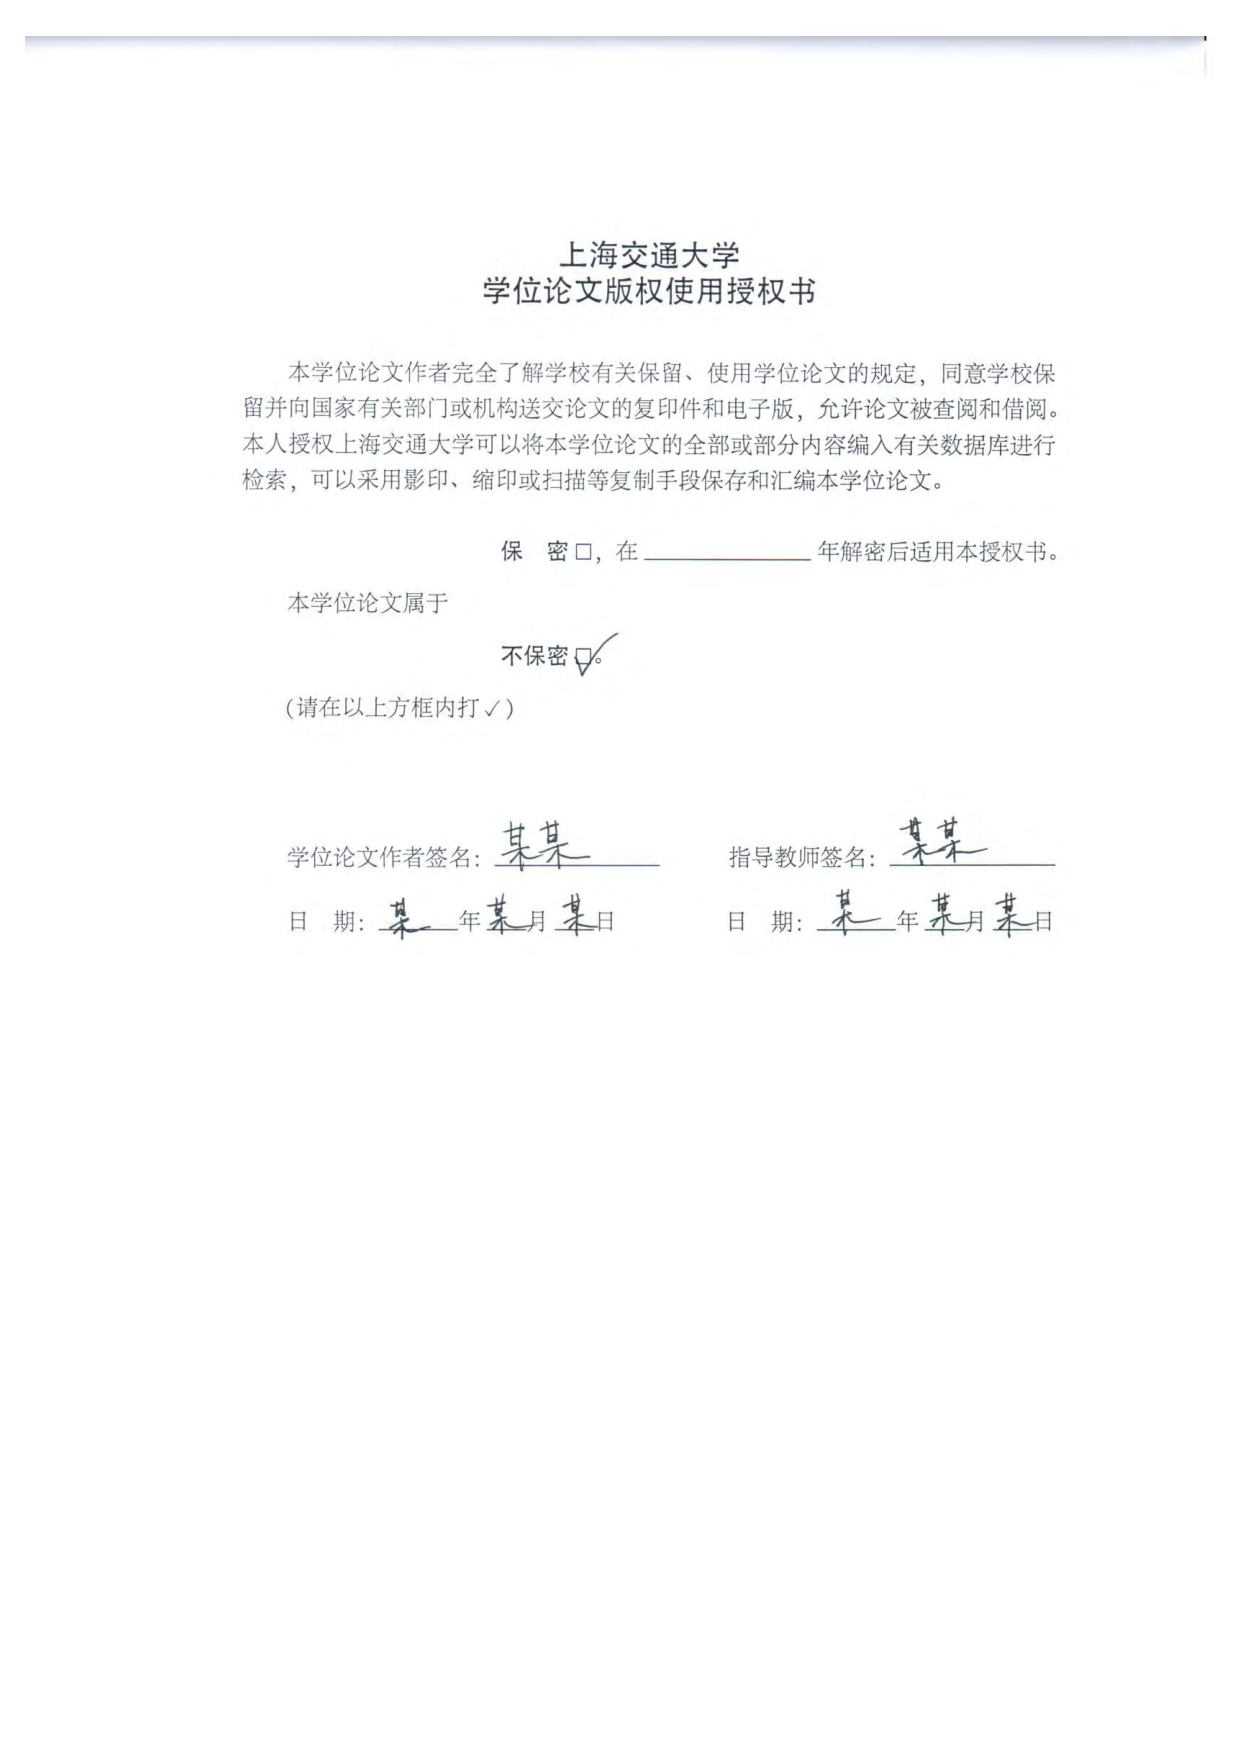
\includepdf{pdf/authorization.pdf}
	\cleardoublepage
\else
	\makeDeclareOriginal
	\makeDeclareAuthorization
\fi
\makeatother


\frontmatter 	% 使用罗马数字对前言编号

%% 摘要
\pagestyle{main}
%# -*- coding: utf-8-unix -*-
%%==================================================
%% abstract.tex for SJTU Master Thesis
%%==================================================

\begin{abstract}

图像主观质量评价是人对其通过视觉感知的图像质量在生理和心理上所给出的偏好性的反应。作为一种新兴的媒体,立体图像(Stereoscopic 3D(S3D))凭借感知重建场景深度这一优势,迅速地在家庭、电影院以及其他娱乐产业等领域得到普及。由于平面格式的立体图像/视频在观看过程中因汇聚-调节矛盾容易导致不舒适、视觉疲劳等问题,立体图像的质量评价就显得尤为重要。近年来,随着生理学的发展,人们对人类视觉系统的理解逐步加深,越来越多的研究开始关注人眼视觉特征在图像质量评价方面的作用,一系列很有创造性的基于人类视觉特征的模型被应用到了立体图像质量评价中。眼动数据作为人眼观看图像/视频的直接记录,开始广泛地应用于基于人类视觉特征的模型研究,很好地改善了已有的基于整体图像特征的评价模型效果。但是,这些方法只利用了眼动数据注视区域这一单一特征,而忽略了眼动数据所携带的其他有价值的特征,如注视点的跳变,辐辏调节等。因此,本文的主要目的是对眼动数据做特征性分析,找出与图像质量相关的眼动数据特征,并将其应用在立体图像质量评价当中。

针对这一问题,首先创建了立体图像-眼动数据库(Stereoscopic Image-Eyetracking Data(SIED))。SIED的创建包括了三部分:图像库的建立,眼动数据采集系统开发,眼动实验的设计与实施。SIED的图像是由包括不同场景、不同深度的11幅图像进行了7种出入屏的调整得到的7*11幅图像构成。眼动数据的采集是基于Tobii 眼动仪SDK开发的在线眼动数据采集系统来完成。在线眼动数据采集系统与在线的网络质量评价平台\footnote{\url{http://3dvqa.sjtu.edu.cn/3dvqa}}通信,获取在线发布的测试任务,采集单刺激模式下被试者测试过程的眼动数据,上传主观评价结果及眼动数据。在眼动数据采集过程中,共设计了三个实验,立体视敏度检验实验测试了被试者立体感是否正常;3D校正实验用来获取被试者立体感的系统性偏差,并据此进行眼动数据校正;立体图像的眼动实验采集被试者观看图像时的眼动数据,据此来建立基于眼动数据的立体图像质量评价模型。

为了更好地利用眼动数据,本文对眼动数据的处理方法进行了研究,在眼动数据的滤波方面,改进了现有的基于双目视点平均位置滤波的2D场景的算法,提出了基于辅眼视点的3D滤波算法。对于眼动数据的3D校正,针对眼动数据采集配置方式的不同,改进了现有的基于视差偏差的校正算法,提出了基于视差角偏差的3D校正算法。同时本文提出了一种立体图像眼动数据可视化的方法——立体图像分层注视密度图法,该方法建立在基于视差图分割的3D图像的分层立体表示方法之上,并在此基础上根据眼动数据的视差角确定注视区域的深度层次,分层创建注视密度图,形成眼动数据的立体可视化表示。其结果可以很好地表示出立体场景下人眼注视的热点区域及其深度。其分层的思想也在后续的特征提取中发挥了重要的作用。

目前还没有基于眼动数据特征的立体图像质量评价模型。针对这一研究现状,本文在对眼动数据处理的基础上,分析研究了眼动数据中所包含的各类特征,主要包括:静态特征、动态特征以及视差角特征。静态特征反映了眼睛的注视结果,用来描述眼睛注视区域的大小,不同区域注视的时长等信息。在此提取的特征包括注视点得个数、注视平均时长等;动态特征主要反映了眼睛的运动过程,涉及多个显著性区域间的跳变,眼睛的来回扫视等视觉过程。其特征可以用扫视幅度,扫视次数等来描述;视差角反映了眼睛注视的深度信息以及深度变化信息,与人眼在不同景深区域的调节相关,其特征主要包括了视差角的均值、方差、深度调节幅度等。然后利用SVR回归模型建立了基于眼动数据的立体图像质量模型。模型结果表明,MOS值与眼动数据的特征有很大的关联性,特别与眼动数据的视差角特征的关联更加明显,其与视差角均值的相关度达到0.72(线性相关系数)以上,与深度调节的幅度的关联也达到了0.4以上。因此,利用眼动数据来做立体图像质量评价是可行的。

\keywords{\large 立体图像质量评价 \quad 立体注视真值标注\quad 眼动数据 \quad 立体视觉眼动特征}
\end{abstract}

\begin{englishabstract}

Image Quality Assessment(IQA) is one's reaction for an image that comes into his/her view, which is determined by human physiological and psychological feelings. The image quality plays a key roles in information transmitting that the image carried. As a new medium,  Stereoscopic images (Stereoscopic/3D (S3D)) has an advantage that it can make one feel in the real scenario, which made it quickly spread in household,cinemas and the entertainment industry. Since the stereoscopic image/video has a problem that it makes one feel discomfort and visual fatigue, the quality assessment of it is very important.  Traditional methods of stereo image quality assessment is mainly concentrated in 2D image quality assessment methods applying, 2D image quality assessment plus 3D features such as disparity. In recent years,  The breakthroughs of the human visual system have gradually deepened with the development of physiology. More and more research has been focused on the performance of human visual features in Image Quality Assessment. A series of models  based on human visual features have been creatively applied to assess the quality of the stereo image. In these applications,  eyetracking data is widely used in the model based on human visual features, as a direct record of the movement of human eyes when the eyes are watching images and videos. However, most of the models use the eyetracking data to detect the saliency map of an image and then use the feature of the salient area to replace the feature of whole image. This method can obviously improve the performance of the models that based on the feature of whole image. However, this method only uses the fixation regions labeled by eyetracking data, ignoring other valuable features of  eyetracking data. In our thesis, we aimed at find features of eyetracking data which can be used to the assessment of Stereo images.

To solve this problem, a stereoscopic image database(Stereoscopic Image-Eyetracking Data(SIED)) was created. SIED is composed of 7*11 images. These images are selected from different scenarios and have different depths range. We also adjust their disparity to move objects in images to different depth planes which can create various image quality。meanwhile, the database is useful when we make comparative analysis of eyetracking features that are obtained from different disparity distribution in the same scenario. The collection of eyetracking data is applied the system which is developed by ourselves based Tobii SDK and Qt. The system can collect the eyetracking data  in different models such as test with task or without task. This system was also expanded to some developments specially such as task published online and offline,and the data stored in servers or local,this makes the system applied more conveniently.  In the process of data collection,  three experiments were designed. first, we valid every participant's stereoacurity to make sure they have the normal stereo perception. secondly,  a 3D calibration is applied to get the bias in 3D perception for everyone,  which is used to calibrate the eyetracking data in our main experiment. finally, an experiment that collect eyetraking data under 3D image was shown was designed.The SIED contains 77 stereoscopic images(and their disparity maps), the result of stereoacurity test for all participant and all eyetracking data related to 3D calibration and stereo image.

In order to make use of eyetracking data effectively,the processing methods of eyetracking data were studied,too. We improved the filter and calibration algorithms in 2D regions to fit the 3D fact. At the same time,  a representation of stereoscopic image based on disparity map segmented is proposed, which is the skeleton of our stereo fixation density maps who can show not only the area we fixated,but also the real depth our fixation was.  Some analysis between human visual system and eye movement were done based on stereo fixation density maps,too.

In the end, the eyetracking data features was proposed which contains static features(about fixation area ), dynamic features(related to saccade) and disparity features of eyetracking data,then the SVR regression method was applied to obtain the relevancy between eyetracking data features and MOS values. The results showed that the features of the eyetracking data is related to the MOS values,especially in the disparity features.

\englishkeywords{\large Stereoscopic Image Quality Assessment, Stereoscopic Fixation Density Map, Eyetracking Data, Stereo Eye Movement Features}
\end{englishabstract}



%% 目录、插图目录、表格目录
\tableofcontents
\listoffigures
\addcontentsline{toc}{chapter}{\listfigurename} %将插图目录加入全文目录
\listoftables
\addcontentsline{toc}{chapter}{\listtablename}  %将表格目录加入全文目录
% \listofalgorithms
 %\addcontentsline{toc}{chapter}{代码索引}  %将表格目录加入全文目录

%%# -*- coding: utf-8-unix -*-
\chapter{主要符号对照表}
\label{chap:symb}

\begin{longtable}{rl}

\end{longtable}
 % 主要符号、缩略词对照表

\mainmatter	% 使用阿拉伯数字对正文编号

%% 正文内容
\pagestyle{main}
%# -*- coding: utf-8-unix -*-
%%==================================================
%% chapter01.tex for SJTU Master Thesis
%%==================================================

\chapter{绪论}
\label{chap:overview}



\section{引言}
\label{sec:introduction}
据统计,截止2015年上半年,中国电影3D银幕数量已占全国银幕总数的70\%之多,这标志着中国电影已正式进入3D时代。于此同时,目前市场在售的高清电视机基本都支持3D显示,3D应用越来越广泛。与2D资源类似,立体图像(视频)在应用过程中也要经过编码、传输、存储、解码等过程,这些环节都可能产生图像的失真。因此,在立体图像应用过程中图像质量的测评机制就显得很重要\parencite{galkandage2015full}。和2D图像一样,立体图像质量评价方法有主观评价和客观评价之分,受限于高昂的时间和人力成本,主观评价并不适用于工业生产领域,这使得基于图像自身特征的客观质量评价方法在计算机速率迅速提高的背景下得到了广泛应用,因此,提升客观图像质量评价方法的性能至关重要。而客观质量评价方法的效果则需要以主观评价结果来衡量,所以,主客观图像质量评价方法的结合是科研领域的重要方法之一。

近年来立体图像质量评价方法开始从直接的图像特征提取向引入人眼视觉特征转变\parencite{bensalma2013perceptual,engelke2011visual,hachicha2013stereo,ryu2014no}。引入视觉特征的其中一个方法就是利用眼动仪来标记用户的注视区域,从而用注视区域的特征取代整体图像的特征\parencite{ninassi2007does}。这种方法很好地提升了现有的基于图像特征的立体图像质量评价方法的效果\parencite{liu2009studying,liu2011visual}。但是,这些研究方法并没有考虑眼动数据自身的特征,作为眼睛运动过程的记录,眼动数据本身的特征并没有受到重视。因此,本文将研究眼动数据自身的特征与立体图像质量之间的关系。

\section{论文研究的背景及意义}
\label{sec:background}
图像质量评价的过程是视觉系统对看到的图像进行处理后得到的好恶判断的过程。眼睛注视到图像后,其接收到的信息进入视觉系统,大脑皮层对图像进行特征提取、编码,最后在中枢神经系统进行融合、成像\parencite{zhu20143d}。由于人眼视觉系统经过长时间的进化,对所见事物有经验的积累,当大脑皮层重构出所看事物的像后,大脑会从主观上将看到的图像与积累的经验进行对比,从而对图像做出优劣判断\parencite{liu2010scene},这个过程可以以图\ref{fig:pycologyprocess}来表示。因此,起初的图像质量评价具有经验性的特点。随着工业科技的发展,人们在工程实践中发现亮度、色度、纹理等特征是影响图像质量的重要因素,所以,图像质量评价的方法转向图像特征的提取上,这种转变在现代计算机性能逐步提高的背景下很有意义,一系列基于整体图像特征的客观评价方法被提了出来,如PSNR,SSIM\parencite{wang2003multiscale},BLIINDS-II\parencite{saad2012blind}以及基于梯度相似性的IQA\parencite{liu2012image}等,这些算法在2D图像质量评价中发挥了重要的作用。
\begin{figure}[!htp]
  \centering
  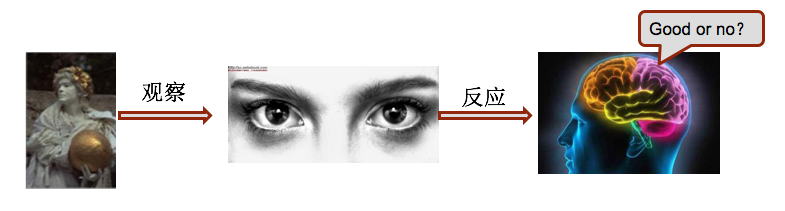
\includegraphics[width=0.8\textwidth]{chap1/pycologyprocess.png}
  \bicaption[fig:pycologyprocess]{图像质量评价的生理过程}{图像质量评价的生理过程}{Fig}{The physiological process of image quality assessment}
\end{figure}

近些年基础科学研究的成果为基于特征的图像质量评价方法奠定了生理学基础。研究表明,图像特征与图像质量关联的原因是视觉系统中存在着处理这些特征的神经与细胞\parencite{hubel1962receptive},更近一步的,人们还发现了大脑皮层处理图像特征的方式与方法\parencite{barlow1967neural,fleet1996neural},这些将在第\ref{chap:humanview}章进行详细描述。这些成果从两方面影响了图像质量评价的发展:一方面是人们意识到影响图像质量的并不是图像的整体,而是进入视觉系统的部分,因此,图像特征的提取从整体转向了局部;另一方面是,大脑皮层处理图像的生理过程越来越明了,使得在图像质量评价中模拟人类视觉系统成为一种可能。因此,近年来,基于人眼注视特征的图像质量评价方法越来越多\parencite{wang2002no,zhang2011fsim,wang2004video,chen2006gradient}。眼动数据在这类模型中发挥了重要的作用\parencite{fliegel2008eyetracking,gide2012comparative},特别是2D图像质量评价中,利用眼动数据作为groundtruth标记的注视区域,有效的提升了基于特征的图像质量评价方法的效果\parencite{gidevisual,meining2010eye}。正因如此,近年来研究人员开始将眼动数据引入立体图像质量评价中。

相比较2D图像质量评价,眼动数据在立体图像质量评价中可以发挥更大的作用,其理由有三:第一,传统的2D图像质量评价方法在3D图像质量评价中的效果并不太好\parencite{bensalma2013perceptual},而基于人眼注视模型的图像质量评价是目前该领域研究的重点;第二,影响3D图像质量最重要的因素之一是视差,视差涉及双目视觉过程,眼动数据可以记录眼睛的运动过程,可以描述双目视觉的变化过程;第三,观看2D图像时,由于聚焦在屏幕上,眼动数据往往关注两只眼睛的综合功能,而观看3D图像时,两只眼睛看到的是“不同”的画面,此时的眼动数据很有可能描绘这种“不同”。

但是,目前眼动数据在3D图像质量评价中的应用受到了限制,常见的用法还是停留在标记显著性区域,创建人眼注视区域的groundtruth等。造成这种现象的原因比较多。第一,眼动数据在2D图像质量评价中的应用方法已经被证明是有用的\parencite{gidevisual,meining2010eye},因此,直接采用这样的方法的效果是可以保障的;第二,2D图像质量评价经过了长时间的发展,形成了成熟的评价体系,包括研究方法和研究图库等,因此,基于这些图库建立了较完备的眼动数据集\parencite{winkler2013overview}。而3D图像的整体研究水平并没有到达这样的层次\parencite{bensalma2013perceptual},这无疑限制了眼动数据在该领域的应用;第三,3D下眼动数据的处理技术不完备,目前的眼动数据的滤波、校正、表示等基础技术,基本还是2D场景下处理技术的延续;第四,受限于当前眼动仪的精度,眼动数据标记注视区域时误差精度可忍受,但涉及到视差角等更精细的特征时,其误差较大,这使得当前很少有研究关注眼动数据本身的特征。

从目前已有的研究成果中我们可以发现,眼动数据在已有的2D图像质量评价方法中的效果已经被肯定,但是受限于当前3D领域研究基础比较薄弱与相关的眼动技术无法达到3D特征描述的精度,使眼动仪在3D图像质量评价中的应用受到了限制。其次,作为眼动过程的记录,眼动数据的注视区域特征与图像质量的关联也得到了证实。基于上述分析,我们尝试着来验证眼动数据特征与立体图像质量之间是否存在关联。本文具体的工作从以下三个方面展开:
\begin{itemize}[noitemsep,topsep=0pt,parsep=0pt,partopsep=0pt]
\item 建立立体图像-眼动数据库,为眼动数据特征提取做好准备;
\item 对比分析2D与3D场景下眼动数据基础技术的区别,结合前人的研究算法,给出3D场景下眼动数据的滤波、校正以及表示等方法,并分析其结果;
\item 针对创建的立体图像-眼动数据库,结合上述的眼动数据的处理技术,提取眼动数据特征,并与MOS值进行SVR拟合,讨论利用眼动数据特征评价立体图像质量的可行性。
\end{itemize}

期望通过本问题的研究,可以在创建数据集、基础研究方法等领域做出些许贡献,最重要的是,通过论证眼动数据自身在立体图像质量评价中的作用,拓宽眼动数据的应用领域。

\section{国内外研究现状}
\label{sec:achievement}
图像质量评价经过长期的发展取得了丰硕的成果,2D图像质量评价方法很多论文都进行了详尽的综述,具体可参考\parencite{wang2006modern,gangyi2010overview}。3D图像质量评价总体上可分为三大类:
\begin{itemize}[noitemsep,topsep=0pt,parsep=0pt,partopsep=0pt]
\item 2D图像质量评价方法的直接移植\parencite{wang2003multiscale,watson1993dctune,miyahara1998objective};
\item 2D图像特征加3D信息(深度或视差)的评价方法\parencite{you2010perceptual,tikanmaki2008quality};
\item 基于3D特征的评价方法\parencite{meesters2004survey,cheng20053d}。
\end{itemize}

Rafik Bensalma 对此做了更加详细的综述\parencite{bensalma2013perceptual},这里不再赘述。由于本文的重点是眼动数据在立体图像质量评价中的应用,其中也涉及了眼动数据处理,因此,本文将从眼动数据处理技术、眼动数据在2D图像质量评价中的应用和眼动数据在3D图像质量评价中的应用等三个方面来进行综述。
\subsection{眼动数据处理技术}
\label{sec:eyetracktechnology}
眼动数据来源于眼动仪,眼动仪根据与头部的相对位置关系可分为侵入式(眼睛与眼动仪的相对位置固定,一般为头戴式或固定式)与自由式(头部可在有限范围内相对于眼动仪运动)两大类。为了保证眼动数据的精度,收集数据前需要校正;眼动过程分为注视过程、扫视过程、其他过程(眨眼或眼睛未被捕捉到),为了获取眼动过程,眼动数据需要滤波;为了更好的观看眼动结果,眼动数据的表示也很重要。
\subsubsection{眼动数据校正}
\label{sec:eyetrackcalibration}
无论何种类型的眼动仪,在使用前必须进行校正(calibration)以消除系统误差与个人差异,从而提高测量精度。一般情况下,眼动仪都会原生地带一个2D校正方法,其具体过程如图\ref{fig:calibrationprocess}所示\parencite{nystrom2013influence}。
\begin{figure}[!htp]
  \centering
  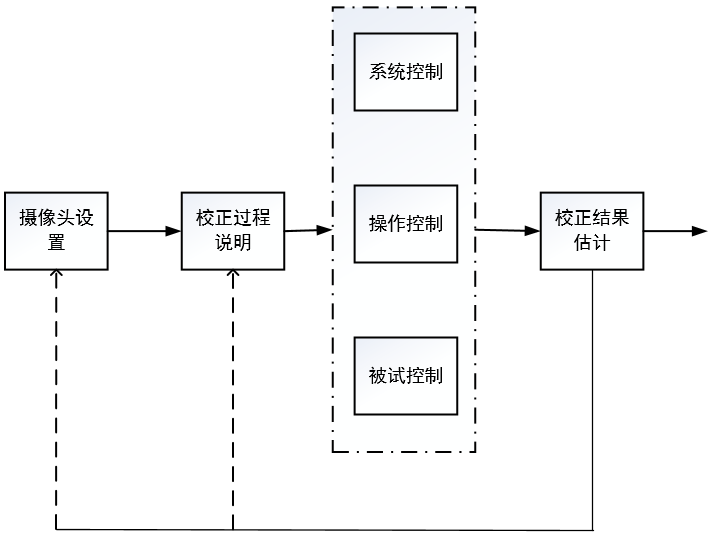
\includegraphics[width=0.6\textwidth]{chap1/calibrationprocess.png}
  \bicaption[fig:calibrationprocess]{眼动仪校正过程}{眼动仪校正过程}{Fig}{The eyetracker calibration process}
\end{figure}
各眼动仪厂家都会给出相应的校正方法\parencite{iview2009system,manual2011v3,manualuser}.

由于眼动仪厂家提供的校正方案只满足用户的基本需求,一些研究工作者对此做了更加精细的研究。迟健男等\parencite{chi2011sight}设计眼动仪时讨论了单摄像机、双摄像机以及多摄像机下的标定过程,最后采用了基于多摄像机全局标定的视线追踪系统来校准眼动仪,实验结果显示其水平误差为$1.5^{\circ}$ ,竖直误差为$1.9^{\circ}$ 。Marcus系统地研究了影响校正效果的各种因素\parencite{nystrom2013influence},包括不同的校正方法、被试者的眼睛生理特征、记录的时刻、注视的方向以及被试者的经验等,最后发现校正过程中提示用户观看目标比让用户自由观看目标效果好,甚至统计的结果还表明眼睛的颜色、睫毛、睫毛膏等也会影响数据的精度,因此,在我们后续的试验中需要避免这些干扰因素。Holmqvist给出了校正过程各个细节的注意事项\parencite{holmqvist2011eye},从目标的的设置、校正过程的操作、校正结果的验证等方面给出了详细的解决方案,这些方案对我们后面的工作具有很高的参考价值。

这些工作的目的是为了提升屏幕上视点的精度,它是为了满足2D场景下的精度要求设计的,这种方法被称为2D校正。由于人眼在屏幕上的注视点可以用左右眼的平均位置估计,所以当双眼误差方向相反时并不会影响最后估计的精度。但是在3D条件下,不仅需要单独估计双眼各自视点的精度,还要利用这两个点去计算双目视差角,所以,仅采用眼动仪自带的2D校准算法是不够的。Wang提出了一种3D校正算法\parencite{wang2014online},该算法在眼动仪原生的2D校正过程后执行。其核心思想是首先计算获得眼动数据的原始视差角,结合预设的视差角,采用拉格朗日最小方差的方法就可以获取系统偏差系数,从而利用该系数校准实验数据。Essig提出了一种叫做Parametrized Self-Organizing Map (PSOM)的方法\parencite{essig2006neural},该方法利用神经网络学习获取2D注视点到3D注视点的映射关系,然后从3D注视点获取深度信息。Pfeiffer在多个数据集上验证了普通的深度几何模型与PSOM的精度,得出了PSOM有更好效果的结论\parencite{pfeiffer2008evaluation}。这些方法在一定程度上提升了数据在3D意义下的精度,但是在实际使用中都有局限性,Wang的算法基于普通的深度几何模型,只适用于头部固定的眼动仪,而PSOM过于复杂,且时间效率不高。所以,在本文的前期工作中\parencite{ma2015new},对Wang的算法进行了改进,基本满足了精度与效率的要求。
\subsubsection{眼动数据滤波}
\label{chap1:sec:filter}
虽然不同公司生产的眼动仪略有差异,但是提供给用户的数据都比较类似。以Tobii眼动仪为例,用户可以获得实时的时间信息、屏幕上的注视点坐标、眼睛的位置坐标、双目距、瞳孔直径、眼动仪运行状态等信息。眼动数据处理的目的是获取人眼观看时的三种状态,即注视过程、扫视过程、眨眼等未知过程。因此传统的滤波方法是利用低通滤波器平滑眼动过程,然后采用聚类的算法分离眼动过程。Zhu提出了一种实时滤波的方法\parencite{zhu2002combining},首先利用Kalman滤波器追踪眼球,然后利用Mean Shift方法进行聚类。
Peng也做了类似的工作\parencite{peng2005mean}。Duchowski给出了眼动过程的分析方法\parencite{duchowski2007eye},深入讨论了信号去噪、注视点检测、扫视点检测等方法,这些方法为后续的研究做出了很重要的贡献。从工程实践的角度来看,Olsson为Tobii开发的滤波算法\parencite{olsson2007real}具有简单易实现、精度高的特点,其在忽略未知过程的基础上,可以将眼动数据分为注视过程与扫视过程,采用了中值滤波的方法消除高斯噪声,排除异常值的干扰。实验的结果显示,算法在精度与鲁棒性方面都有很高的水平。其他经典的算法还包括I-VT、1-HMM、I-DT、I-MST、I-AOI,Dario D. Salvucci对这些算法做了很好地总结与对比\parencite{salvucci2000identifying}。基于工程实践的考虑,本文的算法改进了Olsson的工作。

\subsubsection{眼动数据表示}
\label{eyetrackdatarepresentation}
获取眼动数据后,一般是以数据库或文本的形式保存,为了直观地观察眼动过程,眼动数据需要做可视化处理。目前最常见的眼动数据的表示方法有灰度图和伪彩色图两大类,前者以明暗程度来度量被注视的程度,后者则以色彩的鲜艳程度来表示,这一类图往往被称作注视密度图。注视密度图通常以高斯噪化的方法,将离散的注视点“模糊化”获取\parencite{wang2013computational}。通过直观地观察眼动数据,往往可以直接总结出眼动运动规律\parencite{kim2014saliency}。除了直观呈现以外,灰度图还可以作为眼睛注视程度的权重。Ulrich Engelke利用这种方法对比分析两个实验室不同被试者观看图片产生的注视密度图,发现即使在不同的实验室,采用不同的眼动仪,利用不同的被试者,其最终的结果在图像质量评价领域具有一致性\parencite{engelke2013comparative}。另外,国内学者也在眼动数据库的构建与可视化方面做出了相应的贡献\parencite{zhang2014dataset}。

这些方法在眼动数据的表示中发挥了很重要的作用,但是作为3D场景下的眼动数据,视差角信息是最重要的信息之一,上述方法无法反应视差角信息。如何表示3D场景下的眼动数据,我们提出了一种新的创建立体图像注视密度图的方法\parencite{ma2015new},更具体的过程将在第\ref{chap:dataprocess}章进行描述。
\subsection{眼动数据在2D图像质量评价中的应用}
\label{eyetrackapplied2D}
眼动数据真的可以提升图像质量评价效果吗?Ninassi对此提出了质疑\parencite{ninassi2007does},他结合了眼动数据的注视密度图和SSIM算法与MAD算法进行了验证,发现眼动数据对于JPEG和JPEG2000失真的图像并没有提升评价效果。但是,后面一系列的成果得出了相反的结论,Fliegel利用了眼动数据标注显著性区域\parencite{fliegel2008eyetracking},进而采用显著性区域的特征代替整体特征,结果发现,眼动数据的应用改进了评价效果。
Liu在这方面也做了大量的工作\parencite{alers2009using,liu2009studying,liu2011visual},其结果表明,无论是将眼动数据用于注视区域标注,还是将眼动数据用于模拟视觉注视过程,眼动数据都可以提升图像质量评价效果。Larson\parencite{larson2008can}利用了5个常见的图像质量评价方法,在两个眼动数据集上进行了验证,结果显示大多数评价方法在眼动数据的辅助下是可以提升评价效果的,更进一步,他们还发现,无任务的眼动数据采集要比有任务的采集效果更加明显。类似的工作还包括\parencite{gide2012comparative},
因此,当前学术界已经基本接受了眼动数据在图像质量评价中具有正面意义这一观点。总体来说,眼动数据在2D图像质量评价中的应用可以以图\ref{fig:eyetrackappliedin2D}来描述,\begin{figure}[ht]
  \centering
  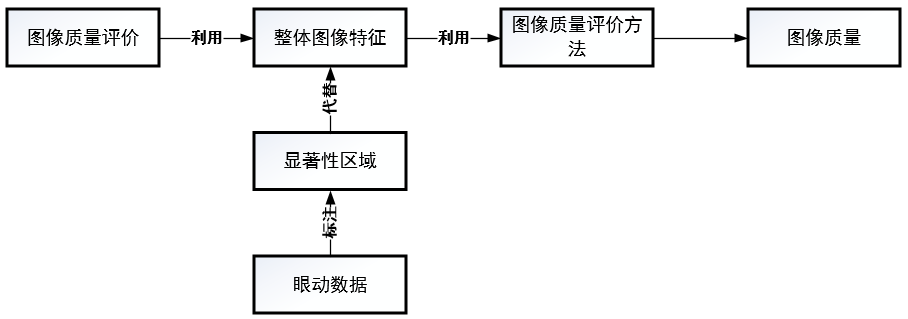
\includegraphics[width=\textwidth]{chap1/eyetrackerappliedin2dimage}
  \bicaption[fig:eyetrackappliedin2D]{眼动数据在2D图像质量评价中的应用方法}{眼动数据在2D图像质量评价中的应用方法}{Fig}{The application of eyetracking data in 2D image quality assessment}
\end{figure}

除了图像方面的应用,眼动数据在视频质量评价方面也发挥了重要的作用。Arndt针对空间域退化的视频,先后获取了眼动数据与脑电图,并以此建立了视频评价的方法\parencite{arndt2014using}。Jia利用眼动数据获取视频的显著性区域,提升了基于模糊和块效应的视频质量评价方法效果\parencite{jia2014no}。

眼动数据在图像/视频质量评价中除了直接获取显著性区域之外,还被作为显著性区域提取算法的ground truth。Yin给出了一种基于相位和幅度差异的视频显著性区域的检测算法,通过眼动数据验证了其精确度\parencite{yin2013video};张\parencite{zhang2013conside}则利用眼动数据验证了当前已有的显著性区域检测方法精度不高,提出了自己的显著性检测算法,并将其应用到了图像质量评价中。
\subsection{眼动数据在3D图像质量评价中的应用}
\label{sec:eyetrackapplied3D}
到目前为止,直接将眼动数据引入立体图像质量评价模型中的方法并不多见。眼动数据在3D图像质量评价方法中的应用与2D图像中的应用类似。第一,用于显著性区域的标注,然后将标注的区域用于立体图像质量评价\parencite{chung2004visual,wang2013computational};第二,用眼动数据验证显著性区域提取算法的精度。Wang利用2D+depth的思想来检测3D图像的显著性区域\parencite{wang2013computational},在提取图像的2D的显著性区域后,利用眼动仪提取了深度方向的显著性区域,二者的交集构成了新的显著性区域。结果表明,这比直接将2D显著性区域提取算法应用到3D图像中效果提升了很多。同时,该工作也贡献了一个3D眼动数据-立体图像库\footnote{ \url{http://ivc.univ-nantes.fr/en/databases/3D_Gaze/?article1103}}。Hanhart则建立了一个包括3D视频和主观评分的数据库\parencite{hanhart2014eyec3d},可以用来做视频质量评价。

值得注意的是,一些新的在立体图像中利用眼动数据的方法被提了出来。Kim利用眼动数据来验证了人眼对立体图像视差的反应过程,其结果表明人眼在低视差域可以很好地注视到显著性物体,相反地,在大视差域却不能\parencite{kim2014saliency}。Liu 的工作类似\parencite{liu2010dichotomy},他们发现人眼更喜欢注视亮度对比度和亮度梯度大的位置,而视差对比度和视差梯度比较大的位置则注视的比较少。这些工作不仅获得了有价值的结论,更重要的是其研究方法是挖掘眼动特征的重要工具。
\section{研究内容和结构安排}
\label{sec:arrangement}
随着人眼视觉模型在立体图像质量评价中发挥的作用越来越重要,眼动数据越来越被重视,除了用来标记人眼注视区域外,眼动数据本身的特征是否与立体图像质量相关就成为一个很有价值的研究问题。

本文的研究内容从立体图像-眼动数据库的创建开始,首先准备了实验所用的图像库,然后设计眼动实验,获取眼动数据。在此基础上,本文将给出3D场景下眼动数据的校正、滤波算法,并给出一种基于视差图分割的立体图像眼动注视密度分层表示方法,这些基础研究保证了眼动数据分析准确度以及合理性。有了这些基本的工具后,本文将处理眼动数据与主观评价数据,包括数据的去噪与异常测试剔除,然后会对眼动实验的结果进行分析。最后本文将基于前人成果和视觉生理过程等提取眼动数据特征,结合主观评分,利用SVR回归模型建立基于眼动数据的图像质量评价模型。

本文将包括六部分,具体安排如下:

第一章绪论,主要讨论课题研究的背景与意义。然后综述眼动数据处理技术,以及眼动数据在2D/3D 图像质量评价中的应用情况,最后对本文的工作做出安排。

第二章描述了人眼注视的生理过程,并以此分析了人眼生理过程与图像质量评价方法的联系。随后,针对我们的研究课题,描述了立体场景下的视差角,给出了眼动数据中视差角的计算方法。

第三章创建了立体图像-眼动实验库,首先选择了11幅内容有代表性的自然场景图像,然后通过视差调整获取了每幅图像的7种变换,最终得到了77幅用于实验的图像。然后设计了实验,实验包括主观评价实验和眼动实验,主观评分实验主要是成对比较实验,为了节约时间成本,将单刺激评分实验与眼动实验合并设计了有任务的眼动实验,眼动实验以眼动数据收集系统的开发开始,该系统既考虑了当前实验的需求,又考虑了以后其他方向的扩展,做好数据收集的准备。整个眼动实验包括三部分,立体视觉正常性检验,校正数据收集,带有主观评分的眼动数据收集等。这样便获取了研究所需素材。

第四章是数据分析,包括主观评分数据的分析与眼动数据的分析两部分,主观数据分析处理的目的主要是去除异常测试,并分析一些初步的实验结果。眼动数据处理则包括了眼动数据的3D校正、滤波以及可视化方法。眼动数据的3D校正过程利用3D眼动实验数据,获取每个被试者深度方向的偏差,并据此对立体图像观看下的眼动数据进行了系统性补偿。眼动数据的滤波过程对眼动数据进行了除噪以及眼动过程分离。眼动数据的可视化表示方法在立体图像分层的表示基础上,对眼动数据注视结果也进行了对应分层,形成了立体注视密度图。最终的实验结果表明以上处理技术是有效的。

第五章是眼动特征提取,眼动特征以前人的研究成果和视觉生理过程为基础来提出。眼动数据的静态特征根据人眼的注视结果提出,这里参考前人的研究成果\parencite{zhang2014application},本文从人眼的注视次数与时长、眨眼次数与时长等方面提取了一部分特征。眼动数据的动态特征则是根据人眼的运动过程来提出的。由于人眼在观看立体图像时视线会在不同区域跳变而产生不舒适感,因此,本文从跳变的幅度,次数等方面提取了一部分特征。视差信息是立体图像的重要信息之一,也是影响图像质量的重要因素,人眼观看立体图像过程中存在深度调整——辐辏调节,这是产生视觉疲劳的重要原因,因此本文从视差角的角度出发提取了一部分特征。然后基于SVR对特征集与主观评分建模,观察并分析了模型结果。

第六章为总结与展望,对本课题的研究内容进行了回顾与总结,并提出可以改进的地方和可能的研究方向。


%# -*- coding: utf-8-unix -*-
%%==================================================
%% chapter02.tex for SJTU Master Thesis
%% Encoding: UTF-8
%%==================================================

\chapter{ 立体场景中的人眼视觉}
\label{chap:humanview}

\section{人眼视觉的生理过程}
\label{sec:humanvisual}

人的视觉系统是双目系统,这就决定了人眼的视觉过程既有单目线索,也有双目线索。单目线索是单只眼睛在观看过程中的生理变化,双目线索既包括单目线索的叠加信息,也存在单目线索的交叉信息。本部分将从这两个方面论述人眼视觉的生理过程,进而论证其与眼动数据之间的联系。
\subsection{人眼单目生理过程}
\label{sec:singleye}

人眼结构如图\ref{fig:eye}所示\footnote[1]{St. Luke’s Cataract and Eye institute, \url{http://www.stlukeseye.com/}},最外层部分分为角膜和巩膜两部分,其中前面1/6的区域为角膜,剩余部分为巩膜。巩膜具有维持眼球形状和保护眼内组织的功能。角膜下方的有色部分称为虹膜,虹膜围绕的区域为瞳孔。光线首先穿过透明的角膜,然后进入虹膜,再到达眼睛的更深处,此时,虹膜会牵引其附着的肌肉来调节瞳孔的大小,以控制进入眼球的光线的量。瞳孔内部是晶状体,其作用是调节眼睛肌肉,使眼睛可以分辨出所看物体的远近。
\begin{figure}[!htp]
  \centering
  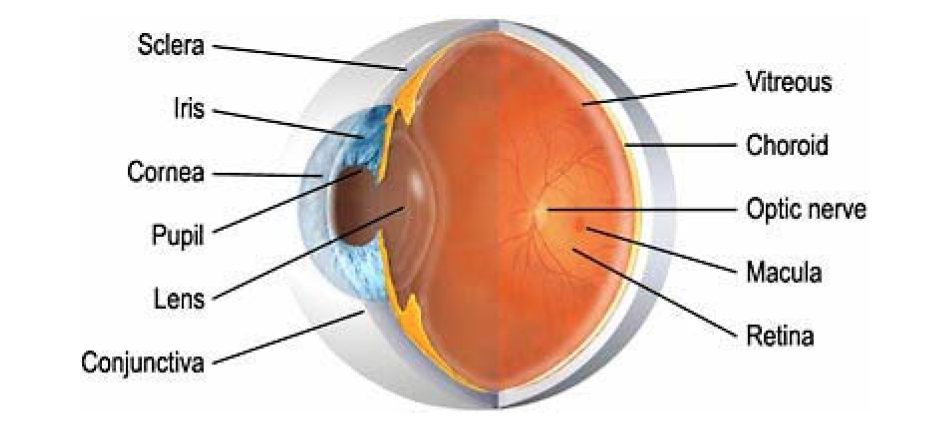
\includegraphics[width=0.6\textwidth]{chap2/eye.png}
  \bicaption[fig:eye]{人眼的生理结构示意图}{人眼的生理结构示意图\footnote[1]{St. Luke’s Cataract and Eye institute, \url{http://www.stlukeseye.com/}}}{Fig}{The human eye\footnote[1]{St. Luke’s Cataract and Eye institute, \url{http://www.stlukeseye.com/}}}
\end{figure}
当人眼观看时,会在眼睛后方的视网膜上形成一幅颠倒的图像。视网膜上包含数量众多的感光细胞----杆细胞和锥细胞,杆细胞的数量约为1亿2000万左右,它不能分辨颜色,但是可以分辨较暗的光线。锥细胞约600万,位于黄斑区内,不仅可以分辨光的强度,而且可以分辨光的颜色,其正常机理需要满足一定的光强度。黄斑中心锥细胞密度最高的区域称为中央凹,这是视网膜中最敏感的部分,人眼大部分的视觉处理是通过中央凹完成的。感光细胞将光刺激转化为电刺激并通过视神经传入大脑,在大脑中还原成所看到的图像\parencite{atchison2000optics}。

单目生理过程表明,眼睛的成像过程其实是眼睛在大脑皮层的指挥下对进入眼球的图像从亮度和色度等维度先进行分解,生成光刺激,在感光细胞的作用下,这些刺激转化为电刺激,从而传入大脑进行处理,这是基于图像特征的图像质量评价方法的生理学基础。同时可以看出,眼睛对进入眼球的信息控制是由眼部肌肉牵引相关部位完成的,也就是说,针对不同的信息,眼睛会通过相关的运动来调节处理。这表明,眼睛的运动过程是大脑对进入眼睛信息量与信息类别控制的结果。这是近年来眼动仪等科技产品被引入视觉研究领域的理论依据。
\subsection{人眼双目生理过程}
\label{sec:doubleye}

人类视觉系统的双目性表明,人眼对所处世界的观察来源于两只眼睛共同作用的结果。眼球的左右移动,使得双目几乎在所有时刻都对同一场景产生出略有差异的两幅图像,通过单目视觉系统,两幅图像首先被感知区域的神经节细胞捕捉,然后会被转移到左右外侧膝状体,最后到达大脑皮层。大脑皮层($V1$ 区域)首先接收到这些信息,这里分布着简单细胞和复杂细胞,简单细胞能够感知方向、大小以及空间频率的相位等信息,同时,为了处理来自双眼的信息,简单细胞会成对工作。而复杂细胞则可以连接两个简单细胞,以此产生双目视觉\parencite{bensalma2013perceptual}。

生理学研究成果进一步表明,简单细胞有单目简单细胞和双目简单细胞之分,同理,复杂细胞也包括单目复杂细胞和双目复杂细胞。Hubel等\parencite{hubel1962receptive}定义了简单细胞的基本概念,它被认为是反应立体视觉中边界、轮廓的关键性元素。同时,简单细胞也被用来做局部空间频率分析。Fleet等\parencite{fleet1996neural}建立了复杂细胞的模型,两个单目简单细胞与一个单目复杂细胞相连接,这两个单目细胞轮流计算同一区域的信号。而一个双目复杂细胞与两组双目简单细胞中的其中之一相连接,这两组简单细胞之间存在着一定的相位差。具体地,简单细胞与复杂细胞的关系如图\ref{fig:simplecomplexcell}所示。这是大脑皮层层次在视觉过程中的生理变化。
\begin{figure}[!htp]
  \centering
  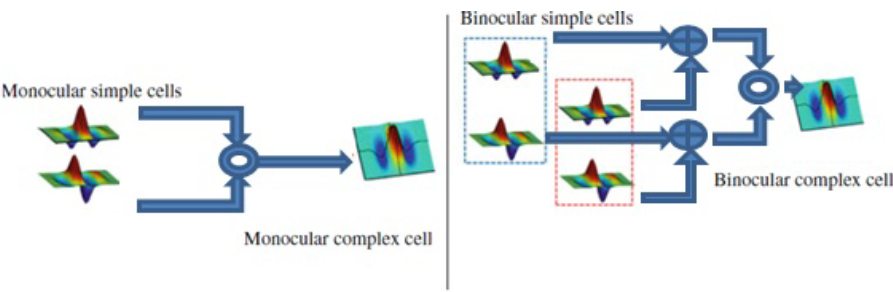
\includegraphics[width=0.8\textwidth]{chap2/simplecomplexcell.png}
  \bicaption[fig:simplecomplexcell]{简单细胞和复杂细胞之间的关系}{简单细胞和复杂细胞之间的关系\supercite{galkandage2015full}}{Fig}{Relationship between monocular and binocular, simple and complex cells\supercite{galkandage2015full}}
\end{figure}

从上述的双目融合过程可以看出,简单细胞与复杂细胞的生理特性与图像的方向、大小、相位、频率等特征相关,使得双目融合成为图像质量评价中纹理、轮廓提取、频域变化等方法的生理学基础。立足于这些生理学基础,科研人员模拟人类视觉过程建立了一系列图像质量评价模型\parencite{bensalma2013perceptual,engelke2011visual,hachicha2013stereo,ryu2014no}。同时,双目视觉过程表明了,只有进入人眼视觉系统的部分才决定了人对图像质量的判断。因此,为了提高特征提取的精度,人眼注视区域的特征也逐步替代了整体图像的特征,这也为眼动仪在图像质量评价方法中得到应用创造了条件。
\subsection{人眼视觉系统对图像视差的处理过程}
\label{sec:disparityprocess}
前面提到,人眼双目几乎在任何时候都会对同一场景产生出略有差异的两幅图像,这种差异我们用视差来描述\parencite{bensalma2013perceptual}。从几何学的角度来看,视差有水平视差和垂直视差之分(以平面正交坐标系为参考)。由于人眼是水平排列的,所以,水平视差在立体成像过程中起决定性作用。人眼对视差的处理结果形成了人类对现实世界的立体感知,这是千百年来人类进化过程中自然场景长期刺激的结果\parencite{liu2010scene}。

人眼对视差敏感的神经元分布在大脑皮层$V1$区域\parencite{hubel1962receptive},最新研究成果发现\parencite{barlow1967neural, nikara1968analysis, pettigrew1968binocular},纹状皮层上也存在着对视差敏感的神经元。研究表明,简单细胞的神经元具有视差选择性,其作用是对一定范围内的视差选择性地做出反应,并且这些细胞会对处理过的视差具有记忆性。这个事实表明,人眼并不是无限制的接纳任意大的视差,当视差超出神经元记忆的峰值之后,人眼并不会有效的对这部分信息进行处理,这与我们在后面的眼动实验中观察的结果是一致的。另外,双目的视差敏感区域并不在视网膜的同一位置,且大小也可能不一样。Anzai等\parencite{anzai1999neural}的研究成果表明,视差敏感神经元还存在相位差,且相位差在双目视差的编码中起主导作用。这也为后面眼动数据的特征提取从频域角度去考虑提供了理论基础。

通过上面对人眼视觉的生理过程的描述,我们可以看出,人眼的视觉过程就是对所看图像的特征提取,然后编码,最后重构的过程。因此,图像质量评价的方法就是模拟人眼视觉生理的过程。通过特征提取,算法拟合,达到测评图像质量的目的。随着生理学的发展,人眼注视模型的研究日益深入,引入注视模型成为近年来图像质量评价的重要方法,眼动数据作为建立注视模型的一个有力地工具便显得日益重要。

\section{立体场景下的视差描述}
\label{sec:stereodisparity}
我们生活的空间是立体的,人眼对立体世界的感知来源于双目接收略有差异的图像。如果双眼的视网膜相同的位置接收到同一点$P$的信息,那么我们就说$P$点的视差为零,且$P$点位于双目视界上。双目视界是人眼的零视差分界面,靠近眼球且在视界内部的称为前景,视界外部的区域则称为背景。通常空间区域的视差角可以用图\ref{fig:commondef:a}来描述\parencite{zhu20143d},以左右眼所在圆周为双目视界(horopter),两条视线的相交形成的角度$\eta$是汇聚角,点$C$的位置比$A$点近,${\phi _l}$ 和 ${\phi _r}$代表了点$C$相对于$A$在视网膜上的位置。如果固定$A$点,则$C$点的视差信息可以表示为视差角:
\begin{equation}
\label{eq:disparitydefine1}
	\delta  = {\phi _l} - {\phi _r}\
\end{equation}

\begin{figure}
  \centering
  \subfigure[双目视界的球面模型的横截面\supercite{liu2010scene}]{
    \label{fig:commondef:a} %% label for first subfigure
    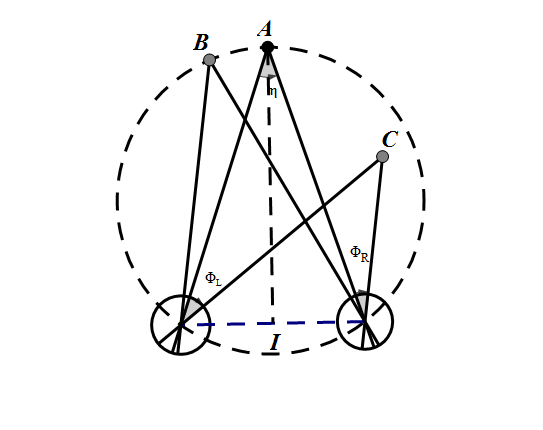
\includegraphics[width=0.4\textwidth]{chap2/horopter.png}}
  \hspace{1in}
  \subfigure[当前双目视界的定义 \supercite{howarth2011geometric}]{
    \label{fig:newdef:b} %% label for second subfigure
    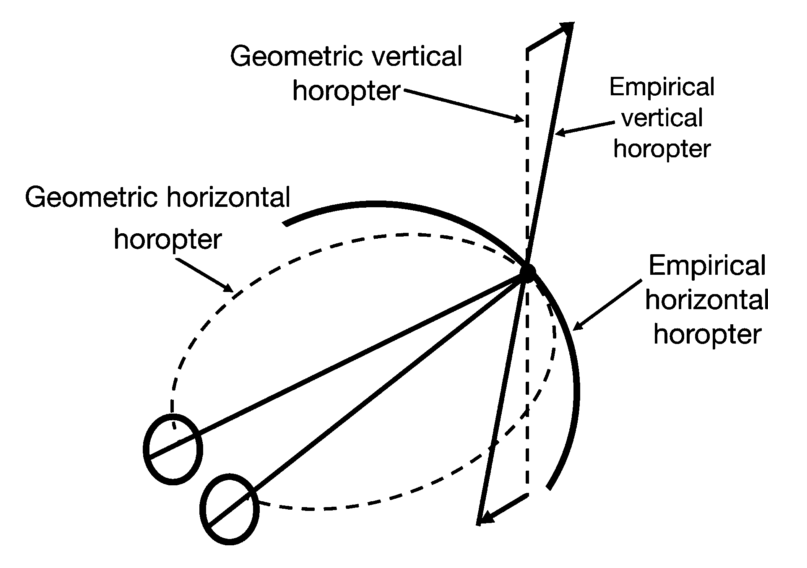
\includegraphics[width=0.4\textwidth]{chap2/modfiedhoropter.png}}
  \bicaption[fig:horopterdefinition]{双目视界的两种定义方式,图a是以前的球面模型截面,图b是最近研究结果定义的几何模型}{双目视界的几何定义}{Fig}{The geometry definition of binocular horopter}
\end{figure}
利用球面建立的双目视界的几何模型可以很好地说明视差角的概念,但是近年来新的研究成果表明,人眼双目视界并不是球面,而是由水平视界和竖直视界组成的综合体。在水平方向上表现为椭球面的一部分,在竖直方向上是一条与水平面呈现夹角的线段----水平面上方远离眼睛,水平面下方靠近眼睛。Howarth \parencite{howarth2011geometric}给出了这种双目视界的定义方法,如图\ref{fig:newdef:b}所示\parencite{zhu20143d}:

进一步地,该研究还表明,双目水平视界的局部曲率很小,竖直视界的夹角也不大。正是这个原因,即使当前主流电视屏幕都是平的,且竖直摆放,也不会造成我们观看的不便,因为电视处于双目视界的局部位置,在水平方向和竖直方向都可以近似认为是“平坦竖直的”。

基于上述分析,我们知道日常生活中电视摆放的位置实质上近似于双目视界所在的位置,因此,在观看3D电视时,由于双目视界在局部范围内曲率很小,所以通常认为电视屏幕就是双目视界,即零视差平面。结合前面对视差角的定义,本文给出在观看3D电视时视差角的计算方法。

主流的3D电视支持多种格式的3D图像与视频,但是最终处理的结果都是左眼看到左图,右眼看到右图,左右眼所看到的图像在水平方向显示差异,这样就会产生水平视差,从而使用户产生出立体感。整个过程实际上模拟了人眼视觉系统。如图\ref{fig:disparitydifinition}所示,假设眼睛$L$,$R$与显示器的中心$C$位于同一水平面,且双眼关于屏幕中垂线对称,$A$,$B$为同一点在左、右图上的位置,当$A$在$B$的左边时,左右眼视线交于屏幕内部,产生入屏效果;当$A$在$B$的右边时,左右眼视线相交于屏幕外面,产生出屏效果;$A$和$B$重合时,双眼视线交于屏幕上,此时所看的场景与2D图像效果相同。3D电视中图像中一点的视差的定义为右眼所看到的该点的横坐标与左眼看到的匹配点横坐标之差,即:
\begin{figure}[!htp]
  \centering
  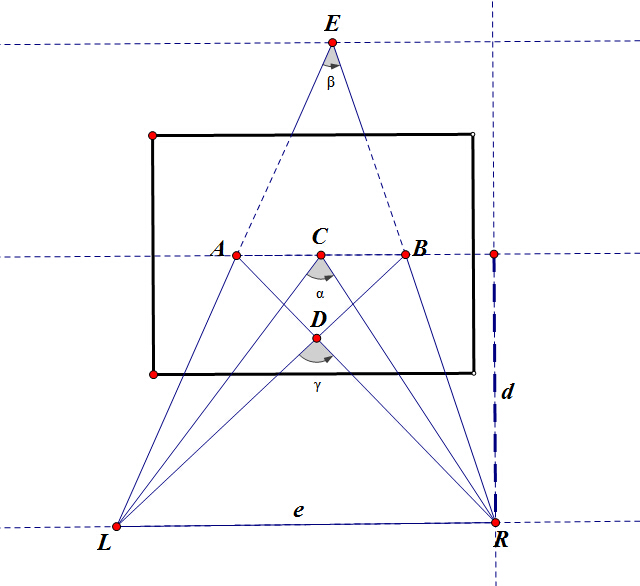
\includegraphics[width=0.5\textwidth]{chap2/disparitydifinition.jpg}
  \bicaption[fig:disparitydifinition]{立体电视下的视差角定义}{立体电视下的视差角定义}{Fig}{Disparity definition under 3DTV watching circum}
\end{figure}
\begin{equation}
\label{chap2:eq:disparitypixel}
D = {x_r} - {x_l}
\end{equation}

这种表示方法可以说明此时场景的出入屏关系,但是不能用来直接描述人眼的立体感知,这是因为人的立体感知与观看环境和人眼双目距相关。因此,视觉中精确的视差信息以视差角来表示。由于屏幕近似于双目视界,因此,这里的视差角可以通过对公式\ref{eq:disparitydefine1}进行变形得到,用$\theta $表示视差角,则视差角可以定义为左右眼视线在屏幕上的汇聚角与左右眼视线的实际汇聚角之差。如图\ref{fig:disparitydifinition}所示:
出屏时视差角:
\begin{equation}
\label{eq:posdisparity}
\theta  = \alpha  - \gamma 
\end{equation}
入屏时
\begin{equation}
\label{eq:negdisparity}
\theta  = \alpha  - \beta 
\end{equation}
这样我们得到了在观看3D电视时视差角的定义。

\section{眼动数据中的视差角计算方法}
\label{sec:caldisparity}
\ref{sec:stereodisparity}概述了观看3D电视时的视差角计算方法,是一种理想状态下的定义。眼动数据的收集也是在观看3D电视时收集的,但是眼动数据来自真实测量,其与理想状况存在以下区别:
\begin{itemize}[noitemsep,topsep=0pt,parsep=0pt,partopsep=0pt]
\item 人眼双目距不再以均值65mm取代,眼动仪会计算出当前测试者的真实双目瞳距;
\item 左右眼视线和屏幕的交点不一定在同一水平线,可能存在竖直视差;
\item 双目关于屏幕中轴未必对称,特别是采用非侵入式眼动仪采集眼动数据时,肯定存在这样的问题。
\end{itemize}

针对以上差异,不同的眼动仪有不同的处理方式。对于头部固定的眼动仪,$Wang$等\parencite{wang2014online}提出了一种简单地处理方法。由于眼睛位置相对稳定,且头部固定支架和屏幕的位置可以摆置得近似对称,同时也能保证眼睛到屏幕的距离为3倍屏高。所以,只需要测量双目距,并利用左右视线与屏幕交点纵坐标的均值代替两个交点的纵坐标,即若$A({x_a},{y_a})$,$B({x_b},{y_b})$为视线与屏幕的交点,且${y_a} \ne {y_b}$,则修正后的交点为$A'({x_a},({y_a} + {y_b})/2)$,$B'({x_b},({y_a} + {y_b})/2)$,这样,所有的条件满足\ref{sec:stereodisparity}的计算方法的要求,利用方程\ref{eq:posdisparity}和\ref{eq:negdisparity}的具体实现方程\ref{eq:chap4:disparitycal}便可以求得结果。

对于头部不固定的眼动仪,如本论文研究所使用的眼动仪,前述处理方法引入的误差会比较大。幸运的是,眼动数据包含了同一坐标系下眼睛位置的坐标以及在屏幕上注视点的坐标,很容易得到视线的向量,这样就可以得到视线的汇聚角,同时用两个交点的平均位置估计中央眼视线在屏幕上的交点,可以算出视线在屏幕上的汇聚角。此时采用方程\ref{eq:posdisparity}或\ref{eq:negdisparity}可以求得视差角,更具体的,如图\ref{fig:realsightline:a}所示,用$O_1$,$O_2$表示双目位置,$G_l$,$G_r$表示左右眼在屏幕上的注视点,则$G_c=(G_l+G_r)/2$是人眼在屏幕上的汇聚点的估计。此时视差角可以定义为:
\begin{equation}
\label{eq:disparityofeyetrackdata}
\theta = \arccos(\frac{{\overrightarrow {{O_1}{G_c}}  \bullet \overrightarrow {{O_2}{G_c}} }}{{\left| {{O_1}{G_c}}
 \right|\left| {{O_2}{G_c}} \right|}}) - \arccos (\frac{{\overrightarrow {{O_1}{G_l}}
  \bullet \overrightarrow {{O_2}{G_r}} }}{{\left| {{O_1}{G_l}} \right|\left| {{O_2}{G_r}}
  \right|}}).
\end{equation}
更一般地,屏幕不同区域视差角的定义方法示意图如图\ref{fig:eyetrackdisparitydifinition:b}。
\begin{figure}
  \centering
  \subfigure[眼动数据测量的实际视线与注视点]{
    \label{fig:realsightline:a} %% label for first subfigure
    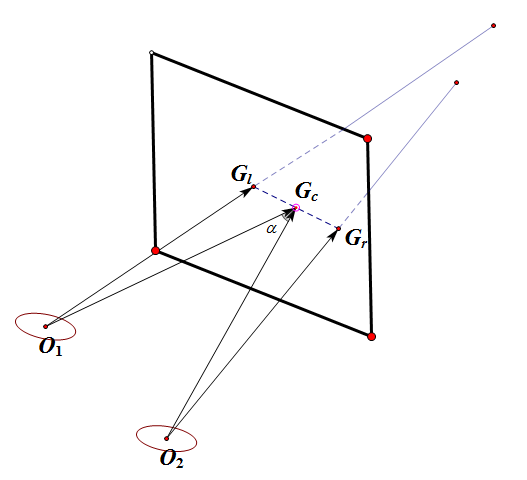
\includegraphics[width=0.4\textwidth]{chap2/angularbysightline.png}}
  \hspace{1in}
  \subfigure[屏幕不同区域的视差角定义方法]{
    \label{fig:eyetrackdisparitydifinition:b} %% label for second subfigure
    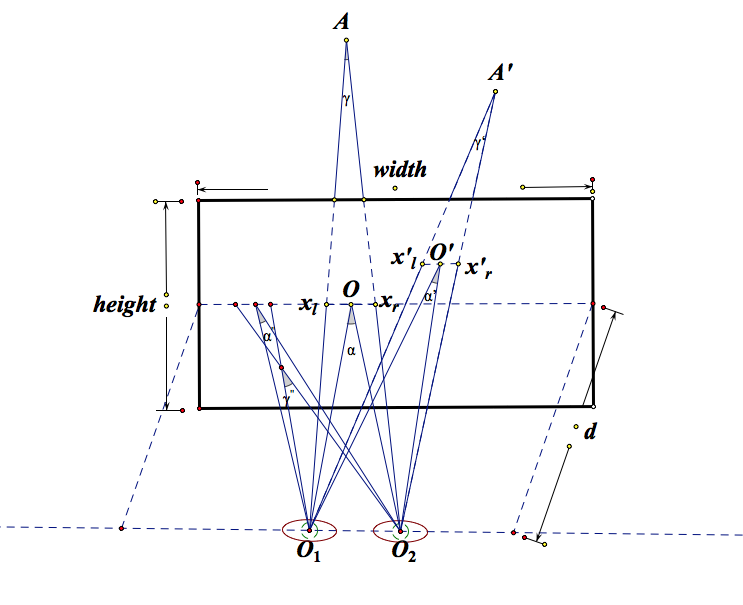
\includegraphics[width=0.4\textwidth]{chap2/eyetrackdisparitydefinition.png}}
  \bicaption[fig:eyetrackrealdisparity]{眼动数据的视差角标示图}{眼动数据的视差角标示图}{Fig}{Disparity definition of Eyetracking Data}
\end{figure}

我们对此稍作说明,如图\ref{fig:realsightline:a},眼动数据会告诉我们双目位置${O_1}$,${O_2}$ 以及屏幕上的注视点$G_l$,$G_r$,此时可以求得左右视线汇聚角$\gamma$,同时利用两个注视点的平均位置$O$,估计视线在屏幕上的汇聚角$\alpha$,这样视差角为$\alpha$与$\gamma$之差。需要说明的是,屏幕的双目视界的特性保证了这种方法不同区域屏幕汇聚角的计算是等价的。

\section{总结}
\label{sec:conclusionchapter2}
本章描述了人眼视觉系统的生理过程。单目视觉系统是光线进入眼睛的第一步,这里负责控制进入眼睛的光的量,同时可以对亮度和色度等特征进行预处理,还完成了光信号到电信号的转化以及电信号的传递。单目肌肉是眼睛运动的动力来源,它使得眼睛可以自由转动以适应各种深度的物体。正是这样的生理特性,构成了眼动仪的生理学基础。双目视觉系统是形成立体视觉的核心,主要由位于大脑皮层V1区域和纹状皮层的简单细胞和复杂细胞完成。此过程是进入视觉系统的信号进行编码的过程,生理学在双目视觉过程的研究成果,是近年来基于人眼注视模型的图像质量评价方法兴起的重要支撑。同时,由于眼睛运动的过程是双目系统处理信息的反馈过程,这也为眼动仪等注视模型的建立奠定了基础。

本文还讨论了双目视觉中特别重要的因素-----视差,在这个过程中,我们发现,摆放在适当位置(一般三倍屏高)的3D显示器实际上是双目视界的一种近似,这从理论上解决了将电视屏幕设为零视差平面的合理性。对于视差角的计算,本文讨论了理想状况与实际情况的联系与区别,结合双目视界的特性,本文给出了眼动数据的视差角计算方法,为后续的眼动数据的应用做好准备。

%# -*- coding: utf-8-unix -*-
\chapter{SIED图像-眼动数据库的建立}
\label{chap:databaseconstruction}
立体图像眼动数据的采集需要三个基本条件:一是用于实验的立体图像;二是需要具有一定精度的眼动数据采集系统;三是合理设计的眼动实验。本章将首先讨论如何选取立体图像,据此建立3D图像库。然后介绍基于Tobii SDK和Qt开发的眼动数据采集系统,简述该系统的设计思考与功能。最后,本文将给出眼动数据采集实验的设计方案以及实验结果,从而创建眼动数据库。
\section{3D图像库的创建}
\label{sec:imagedatabase}
眼动数据的特征与立体图像质量是否存在关联?针对这个问题,首先需要用于质量评价的立体图像,然后在主观评价过程中同步采集眼动数据,最后才能讨论眼动数据的特征与图像质量是否关联。所以我们需要包括不同质量图像的立体图像库。目前已有的3D图像库\footnote{\url{http://stefan.winklerbros.net/resources.html}}大多针对特定失真类型创建\parencite{benoit2008quality,moorthy2013subjective},如\parencite{benoit2008quality}主要研究不同的压缩方式(JPEG and JPEG2000 )对立体图像质量的影响,\parencite{moorthy2013subjective}则讨论了对称失真与非对称失真对立体图像质量的影响的异同。还没有针对影响立体图像质量最明显因素之一——视差创建的立体图像库。因此,本文将创建一个基于视差调整改变图像质量的立体图像库。

影响立体图像质量的因素很多,如亮度、色度、纹理、视差等。变换任意一个因素都将得到不同质量的图像。而亮度,色度,纹理等因素的改变从根本上说是改变了图像的2D特征,这些因素的变化实质上已经改变了图像主体的内容。与它们不同的是,视差特征是立体图像的3D特征,而视差的调整不会造成图像主体内容的改变。更重要的是,图像整体的视差平移会使图像内容出现在不同的景深区域。而同样的内容在不同的景深区域的质量不同\parencite{lambooij2009visual}。根据这一特性,可以对一幅图像进行整体视差调整,使得图像内容展示在不同的深度平面上,以此来获取不同质量的图像,这就是基于视差调整获取不同质量图像的方法,也称之为“移轴”。正如前所述,这种方法有两个优点:一是它不会改变图像主体内容(只对边缘有一些影响),可以消除不同图像内容对图像质量的影响,使影响图像质量的因素变的单一,易于量化控制;二是视差调整对图像质量的效果很明显,易于执行。

针对单一图像进行视差调整可以获取不同质量的图像,但是这种方法不总是可行的。一方面,单一图像在内容上代表性不足,这会使实验结果失去普遍性。另一方面,图像的舒适度是有范围的,在一定的范围内调整视差时,若步长太短,则图像质量的差异并不明显,若步长太长,一幅图像创建的立体图像又太少。因此,我们选取多张图片,然后对每张图像进行一定范围的视差调整,这样就可以获取一定数量的具有代表意义的立体图像库。

我们从3D数码相机拍摄的众多图像中挑选了11张不同场景的图像,图像分辨率为1920x1080,这些图像包括了室内、室外、人物、建筑、雕塑、风景和人造场景等多种场景,图\ref{fig:origImageforexpriment}给出了选取的图像的左图。
\begin{figure}
  \centering
  \subfigure[]{
    \label{fig:26_l} %% label for first subfigure
    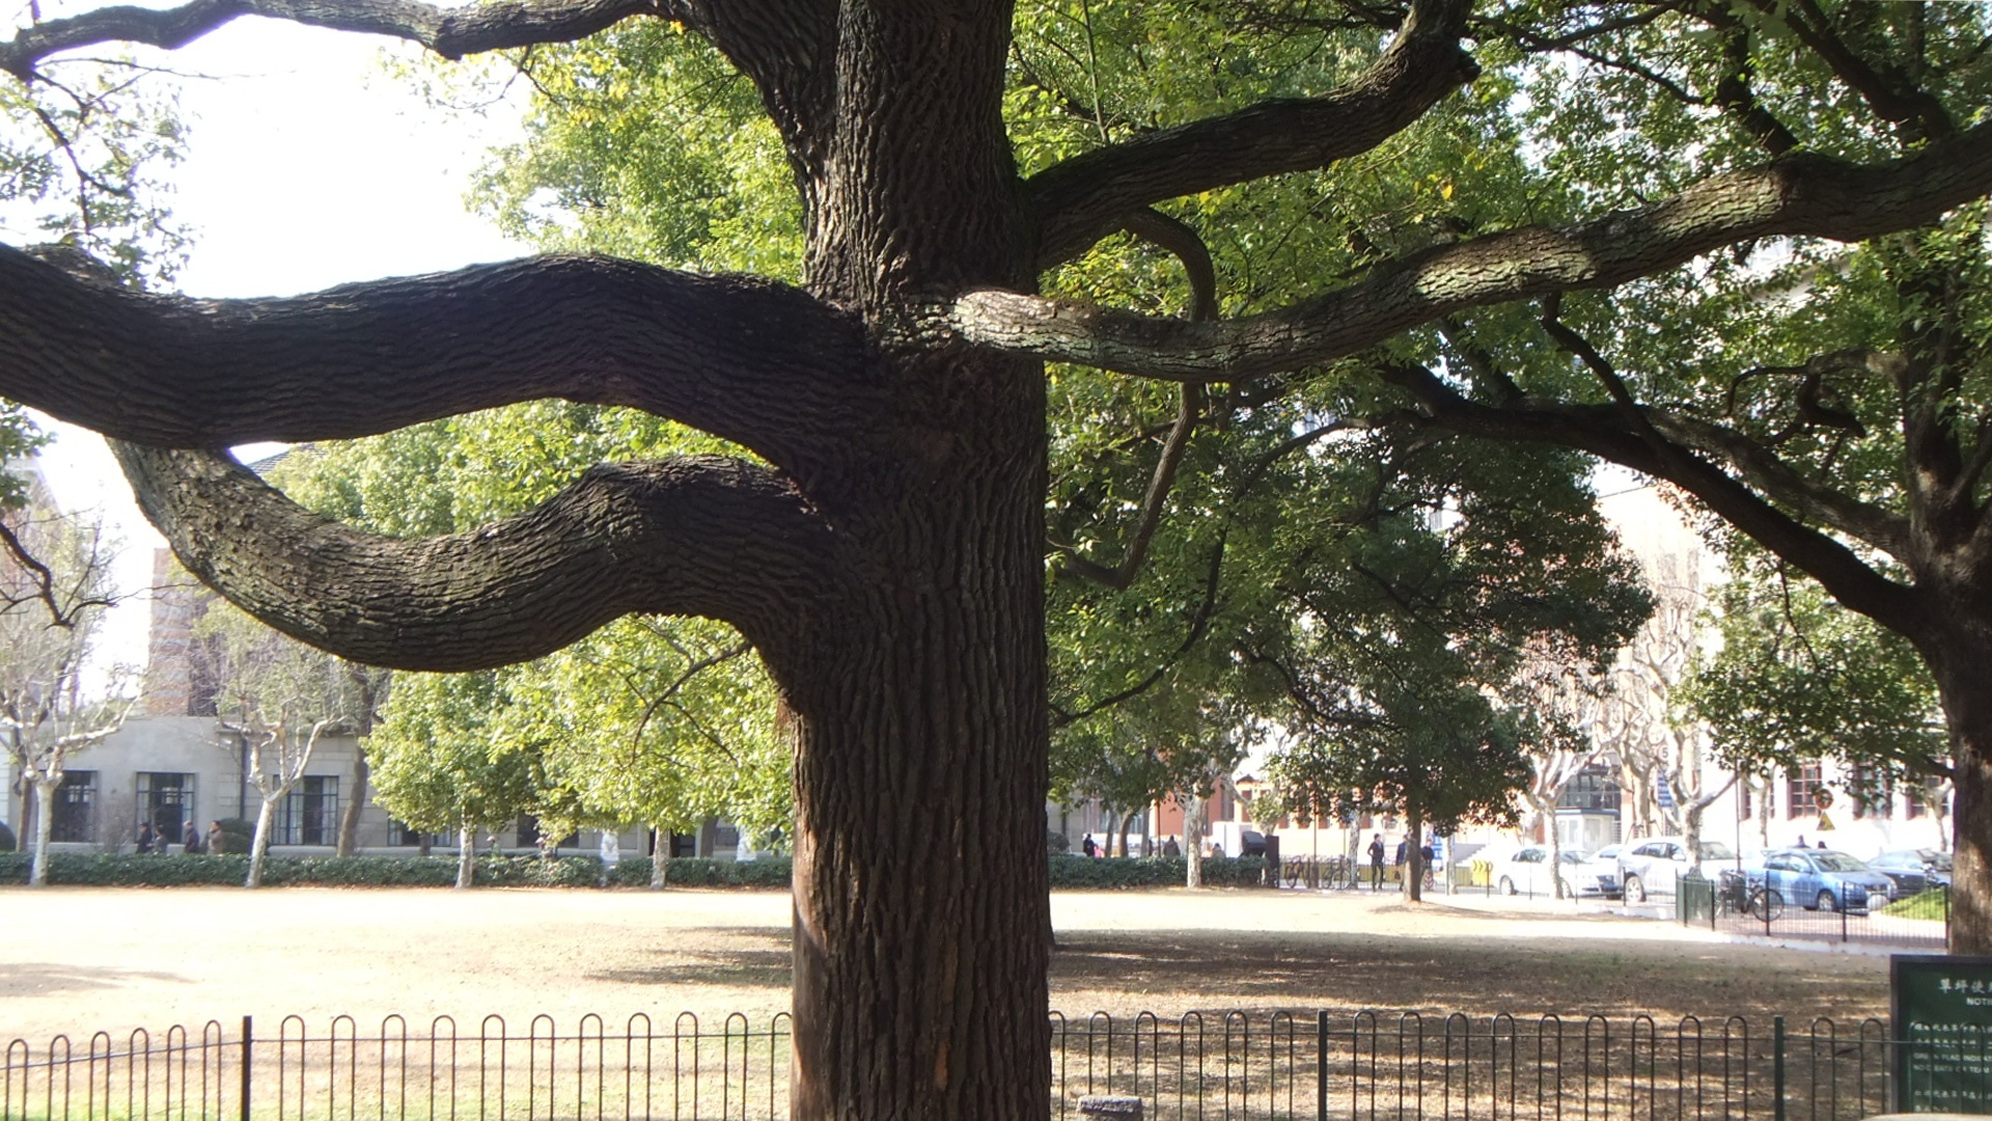
\includegraphics[width=0.3\textwidth]{chap3/26_l}}
  \subfigure[]{
    \label{fig:69_l} %% label for second subfigure
    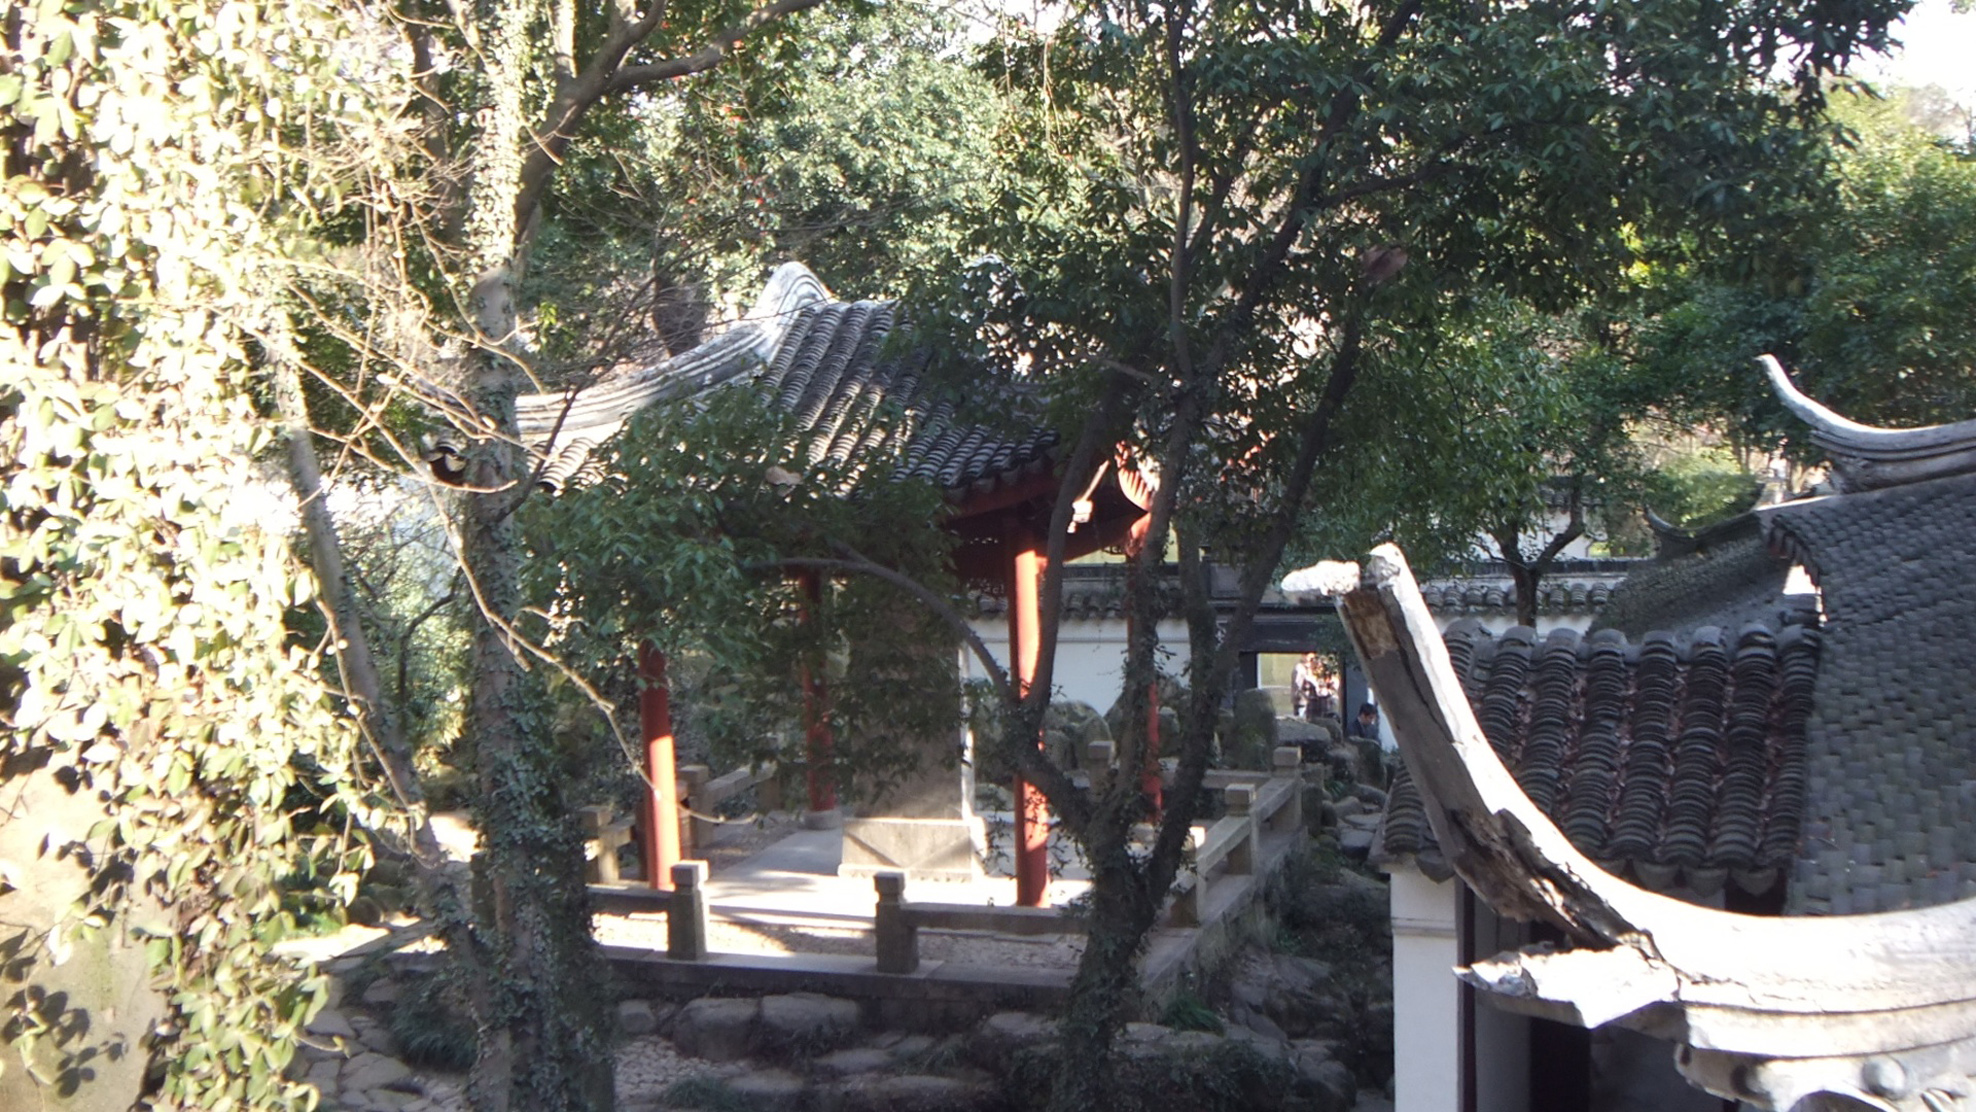
\includegraphics[width=0.3\textwidth]{chap3/69_l}}
  \subfigure[]{
    \label{fig:82_l} %% label for second subfigure
    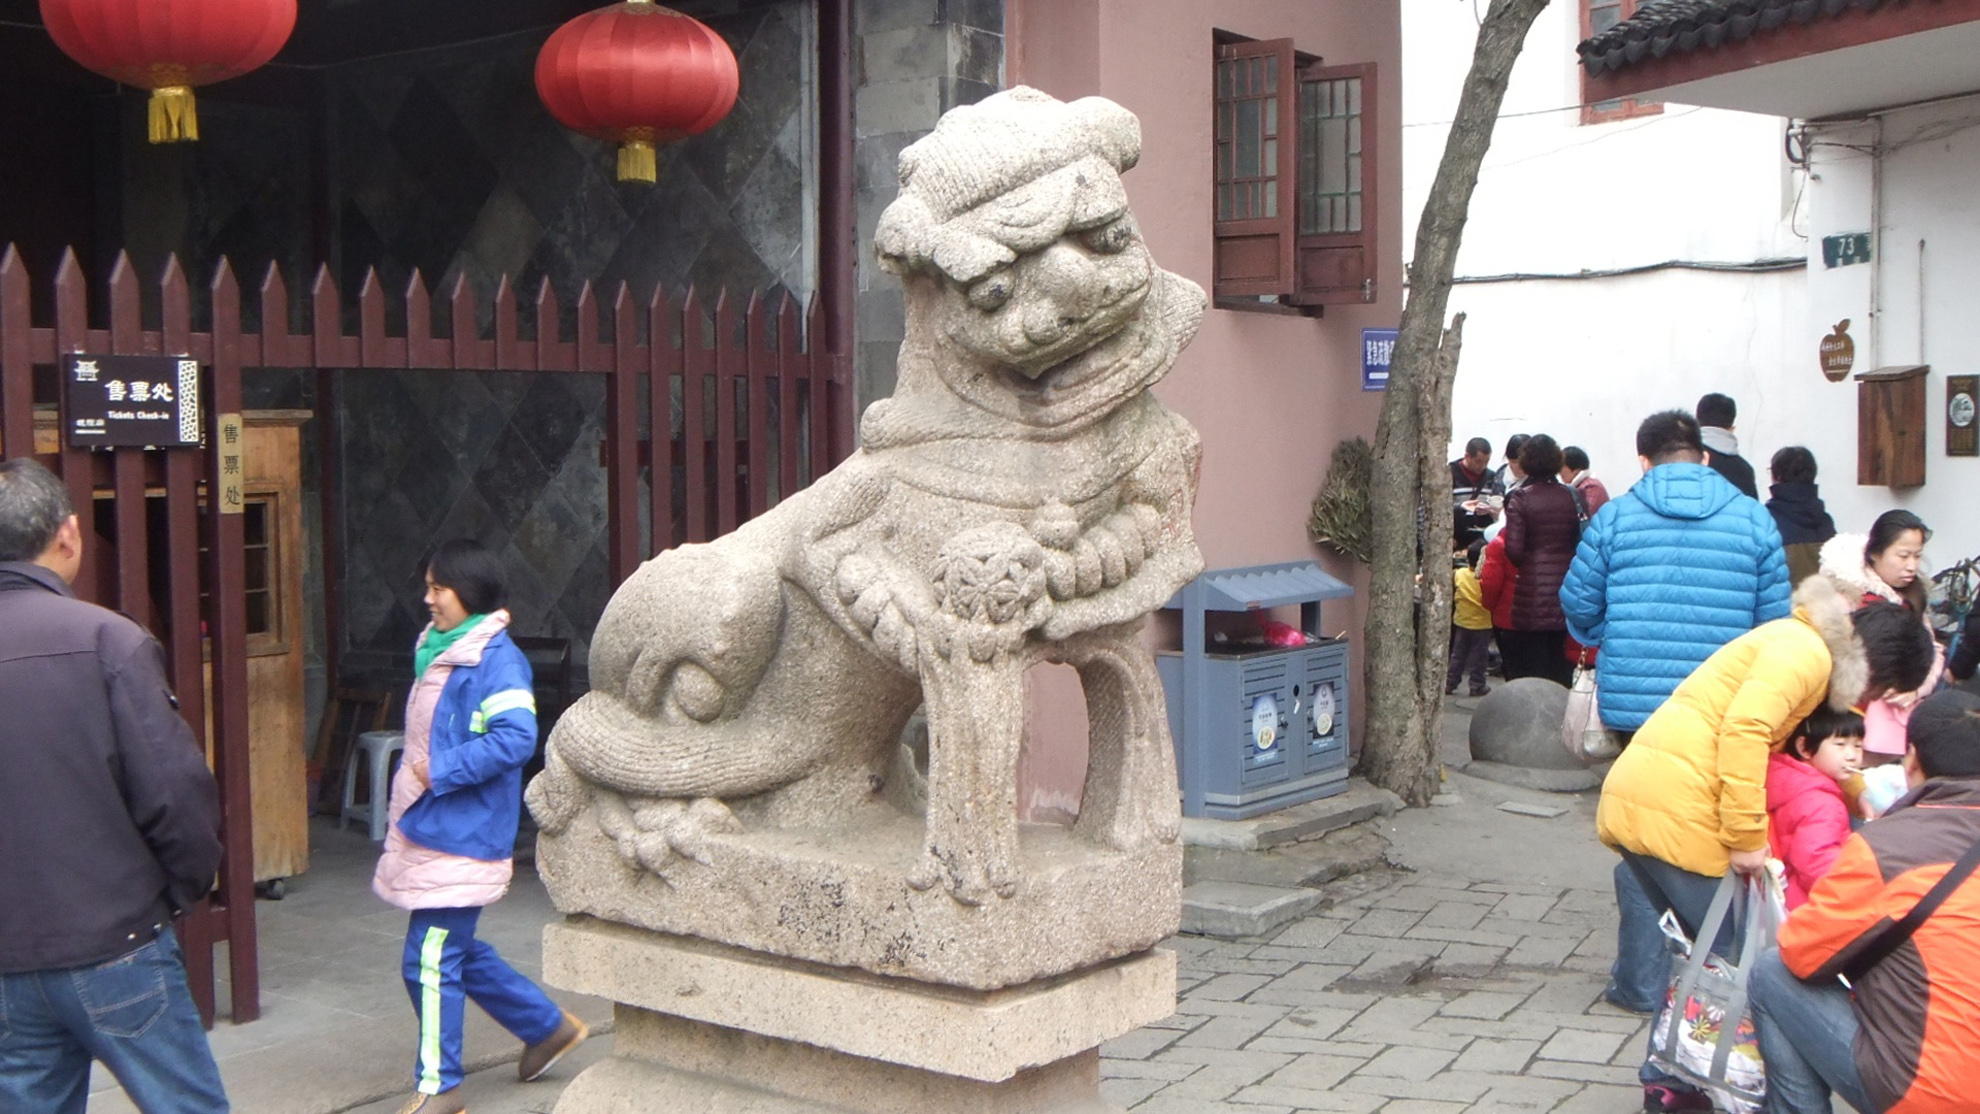
\includegraphics[width=0.3\textwidth]{chap3/82_l}}
    \subfigure[]{
    \label{fig:3_l} %% label for first subfigure
    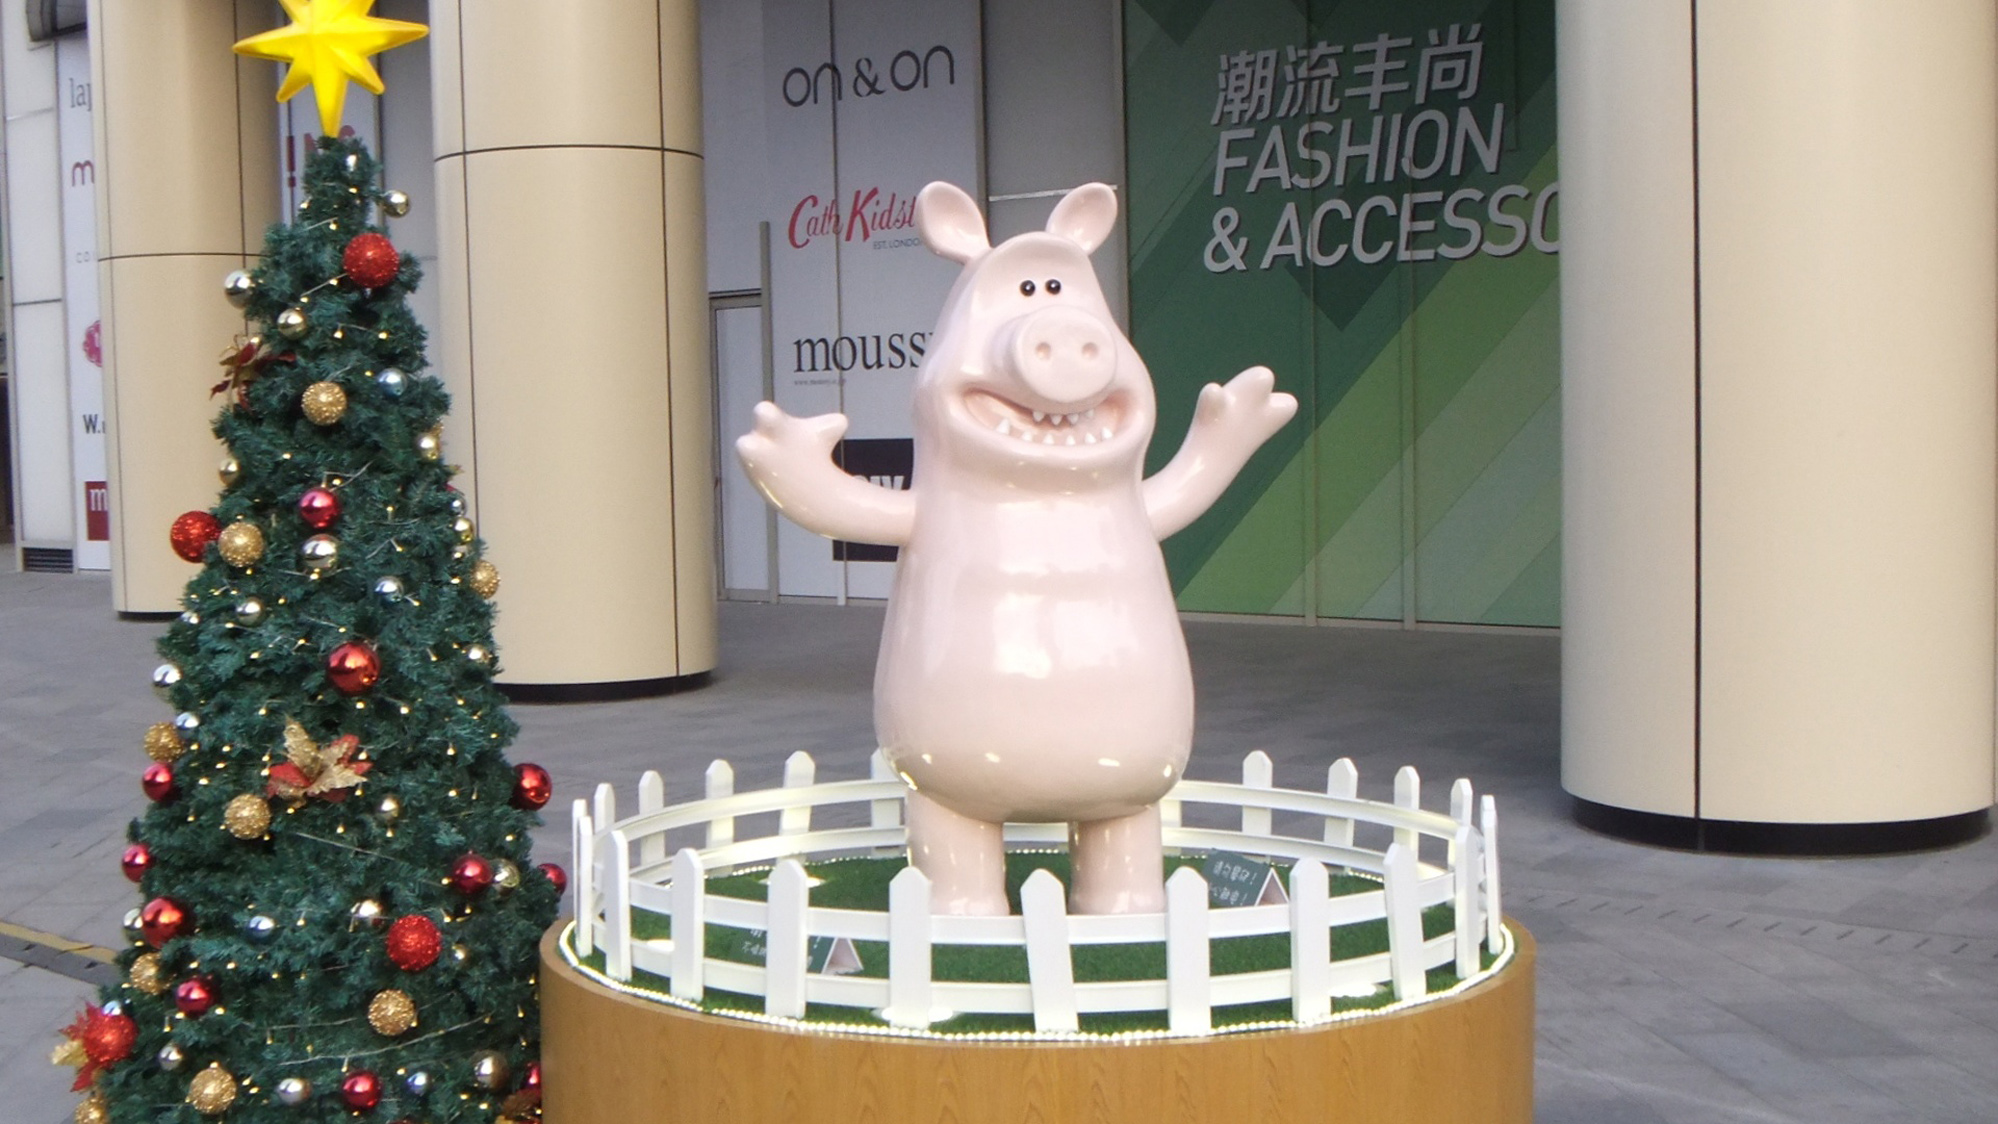
\includegraphics[width=0.3\textwidth]{chap3/3_l}}
  \subfigure[]{
    \label{fig:47_l} %% label for second subfigure
    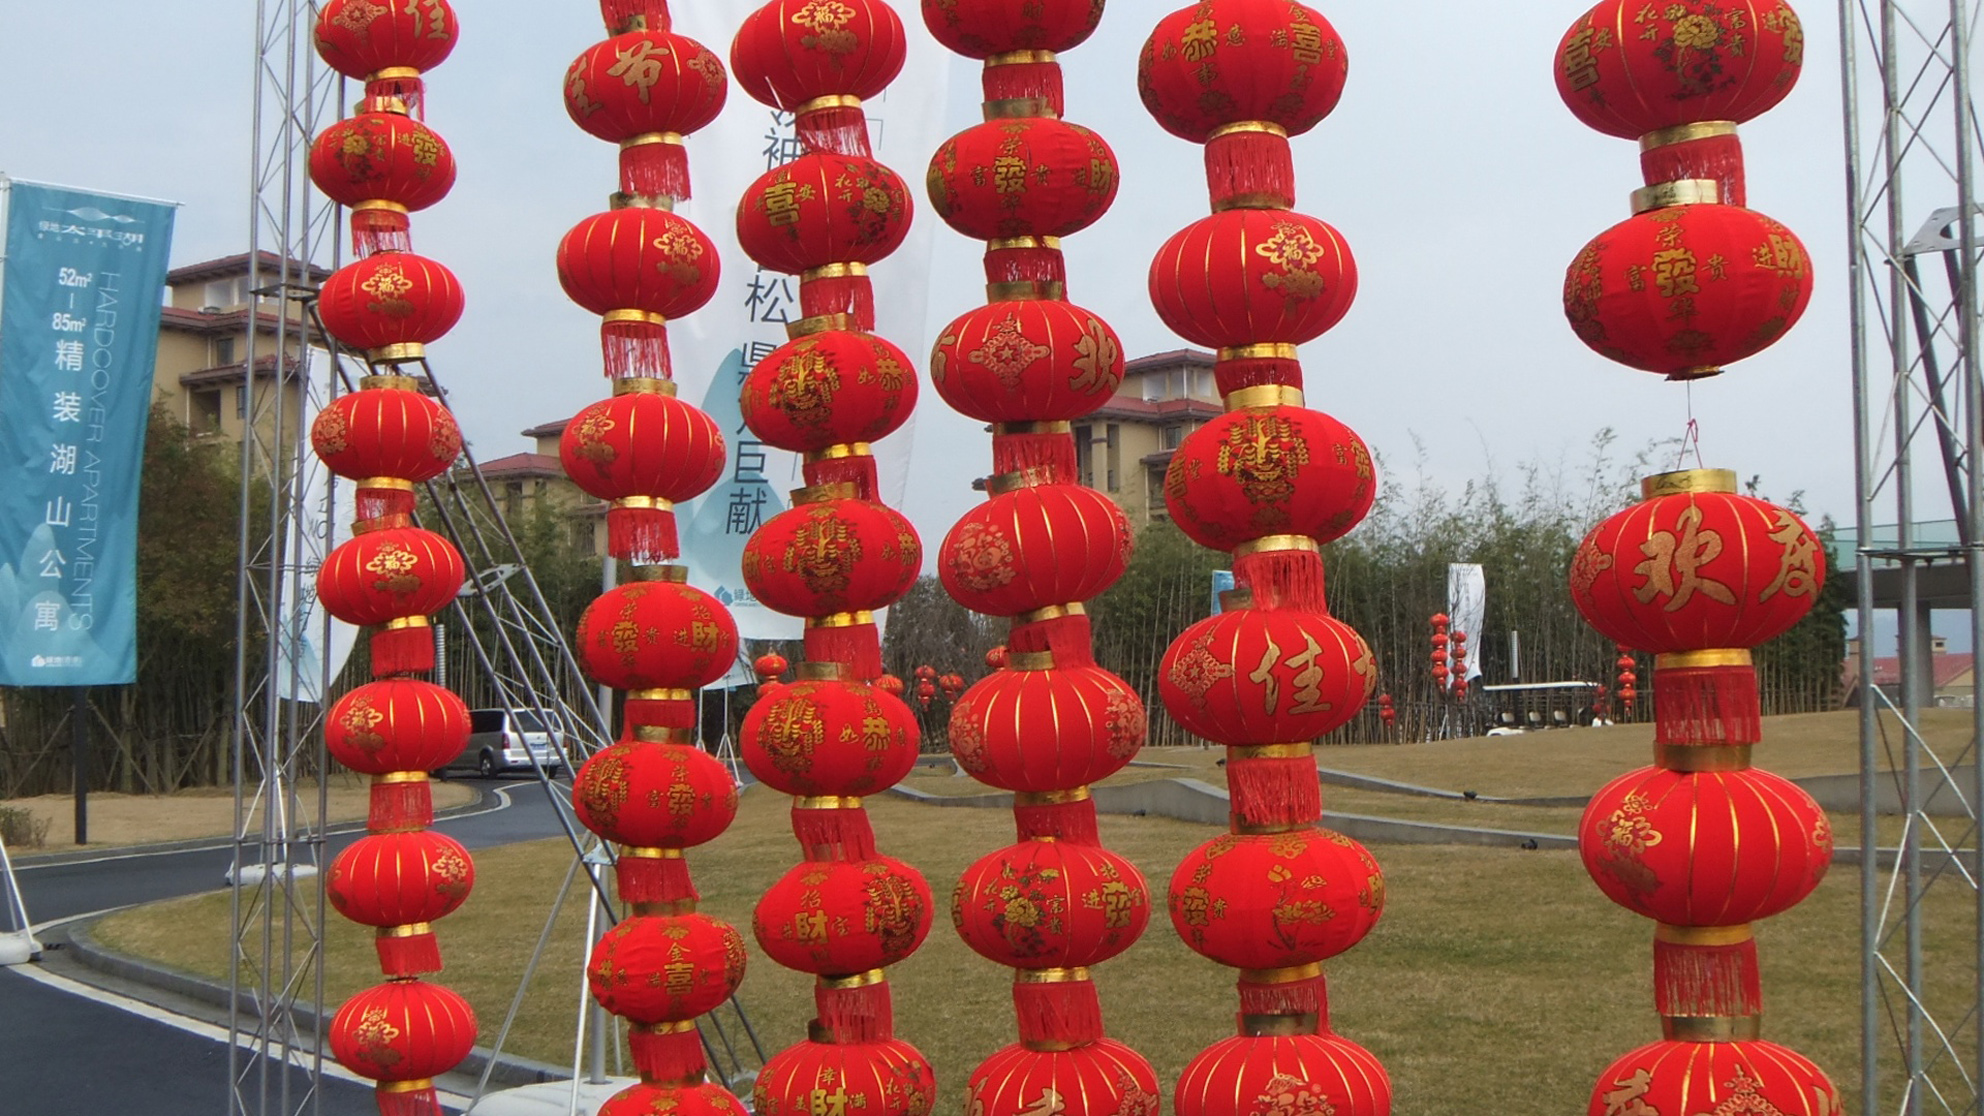
\includegraphics[width=0.3\textwidth]{chap3/47_l}}
  \subfigure[]{
    \label{fig:55_l} %% label for second subfigure
    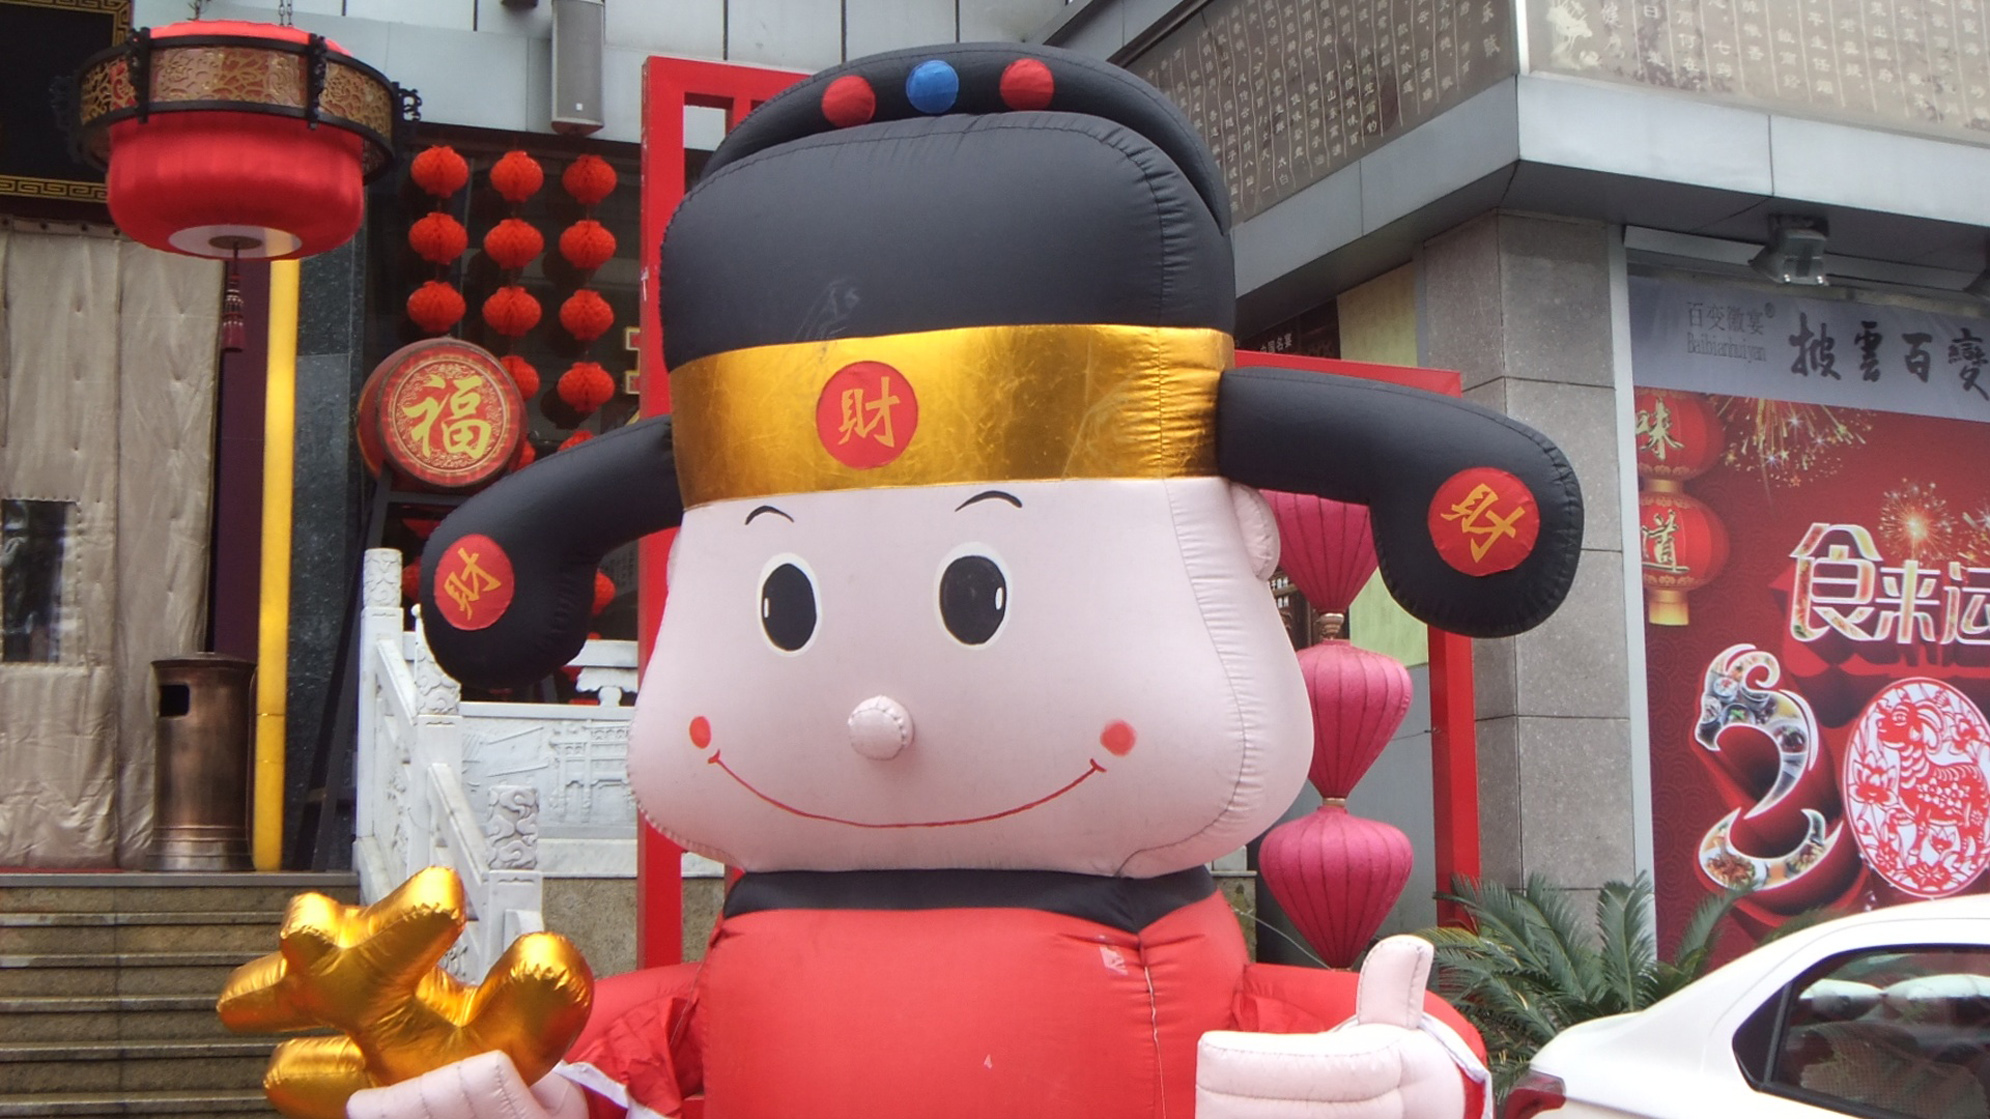
\includegraphics[width=0.3\textwidth]{chap3/55_l}}
    \subfigure[]{
    \label{fig:89_l} %% label for first subfigure
    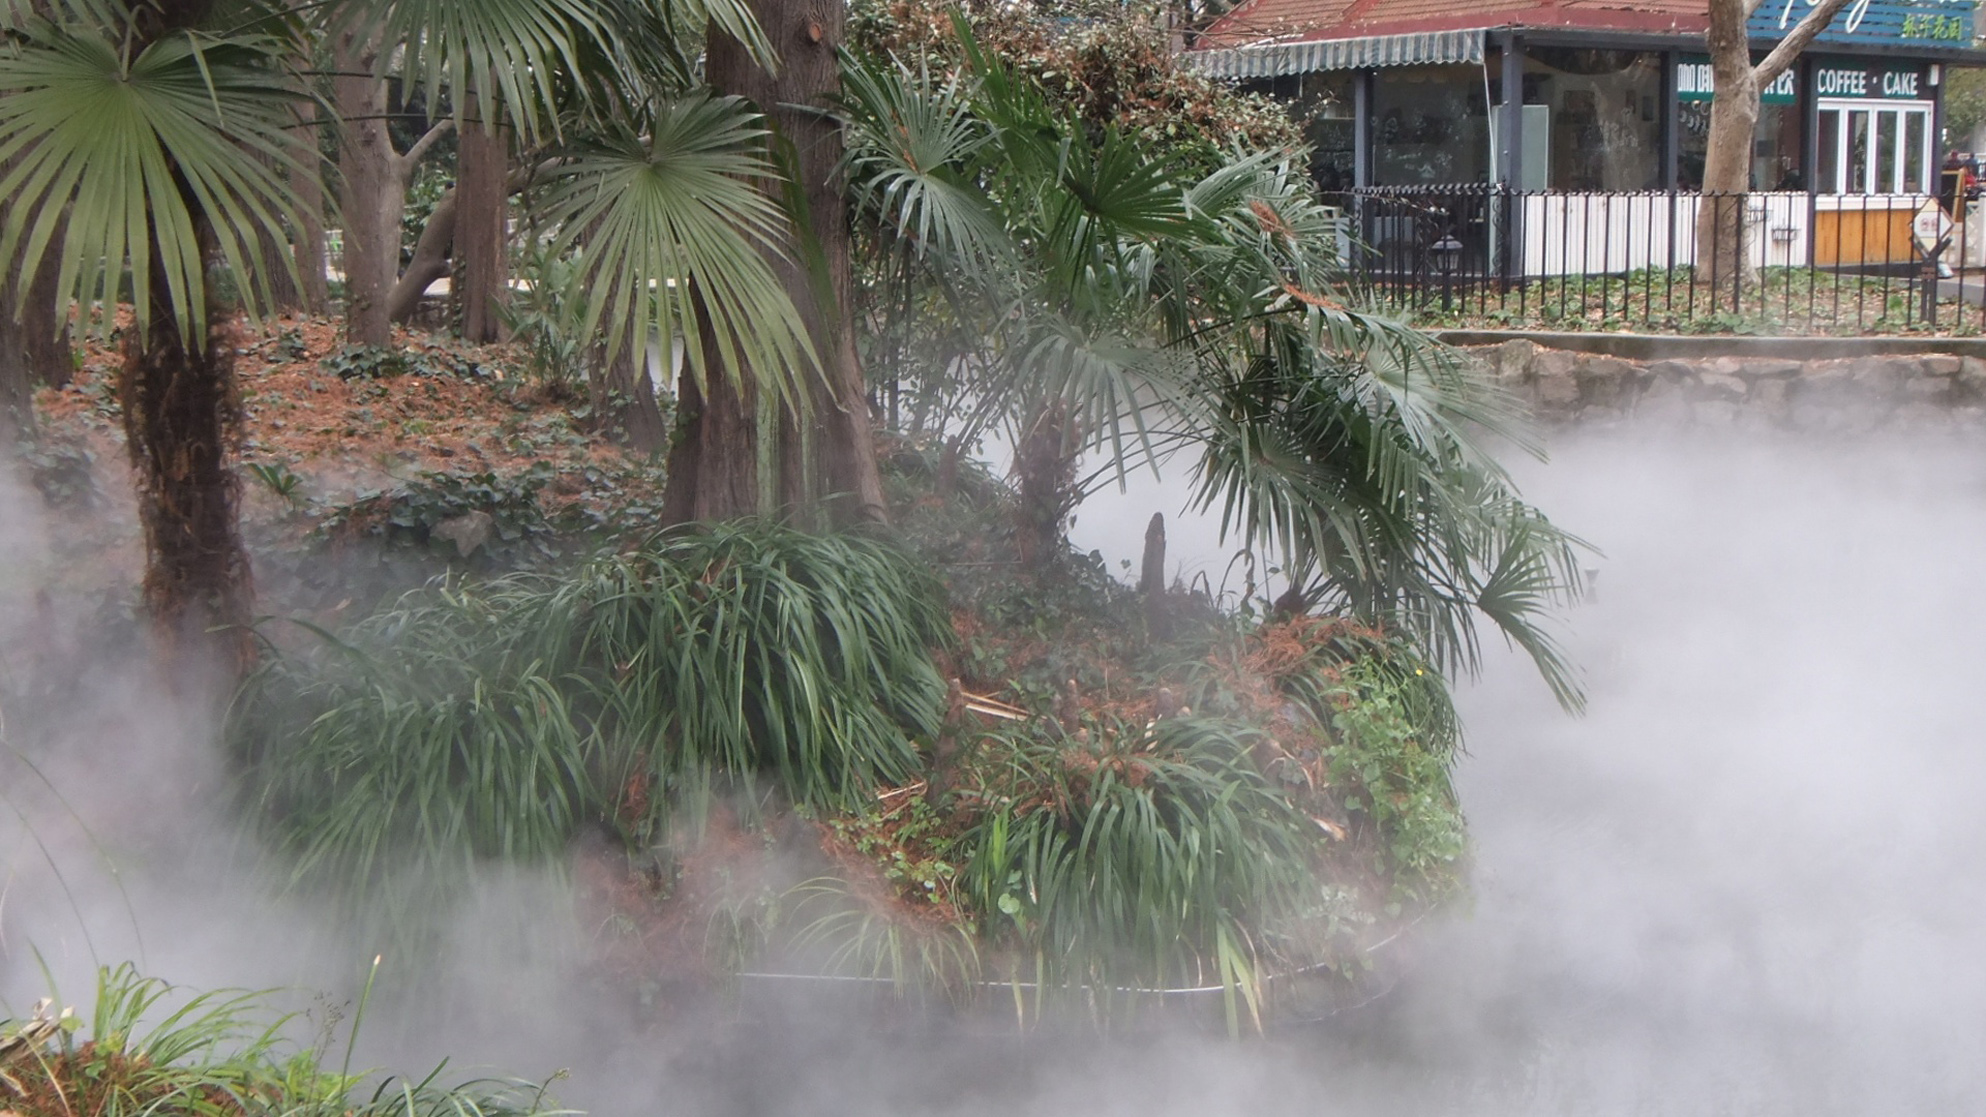
\includegraphics[width=0.3\textwidth]{chap3/89_l}}
  \subfigure[]{
    \label{fig:73_l} %% label for second subfigure
    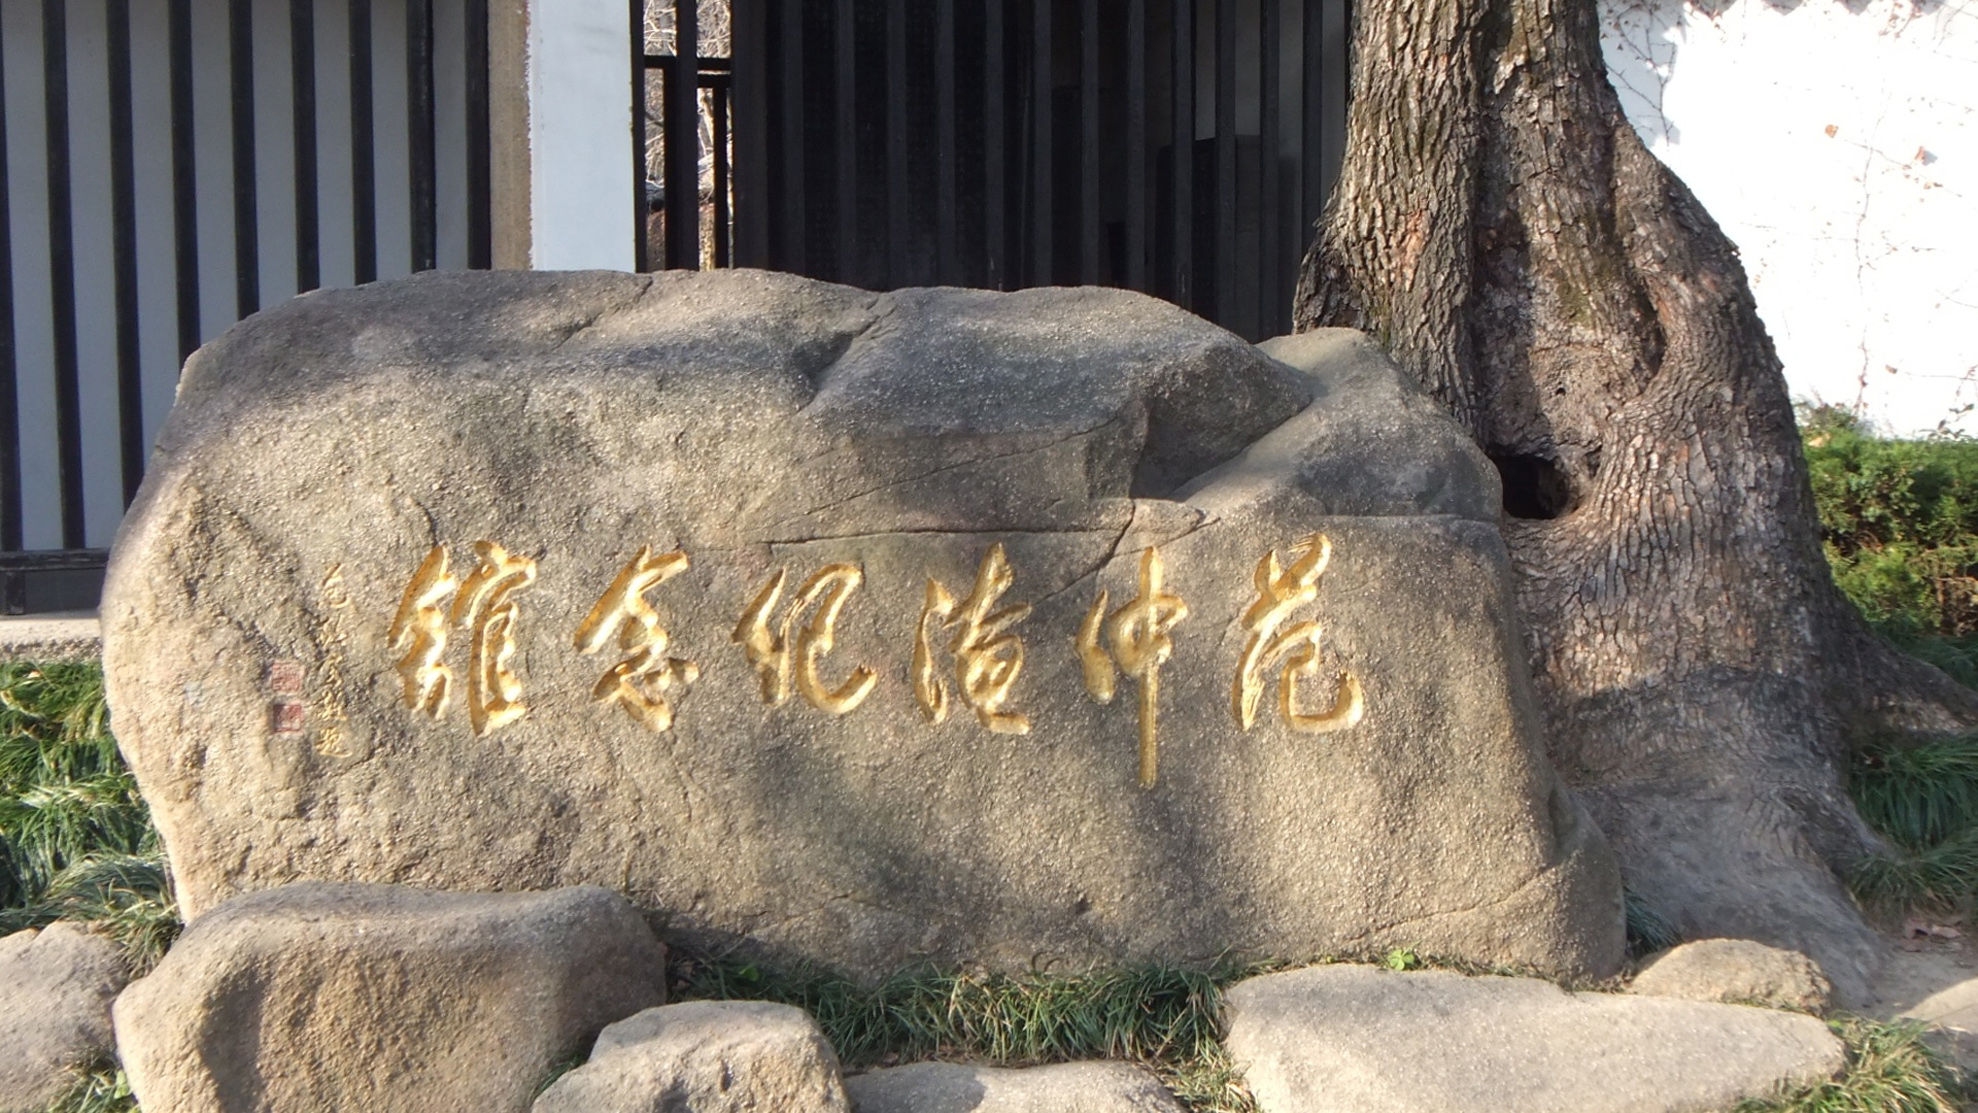
\includegraphics[width=0.3\textwidth]{chap3/73_l}}
  \subfigure[]{
    \label{fig:32_l} %% label for second subfigure
    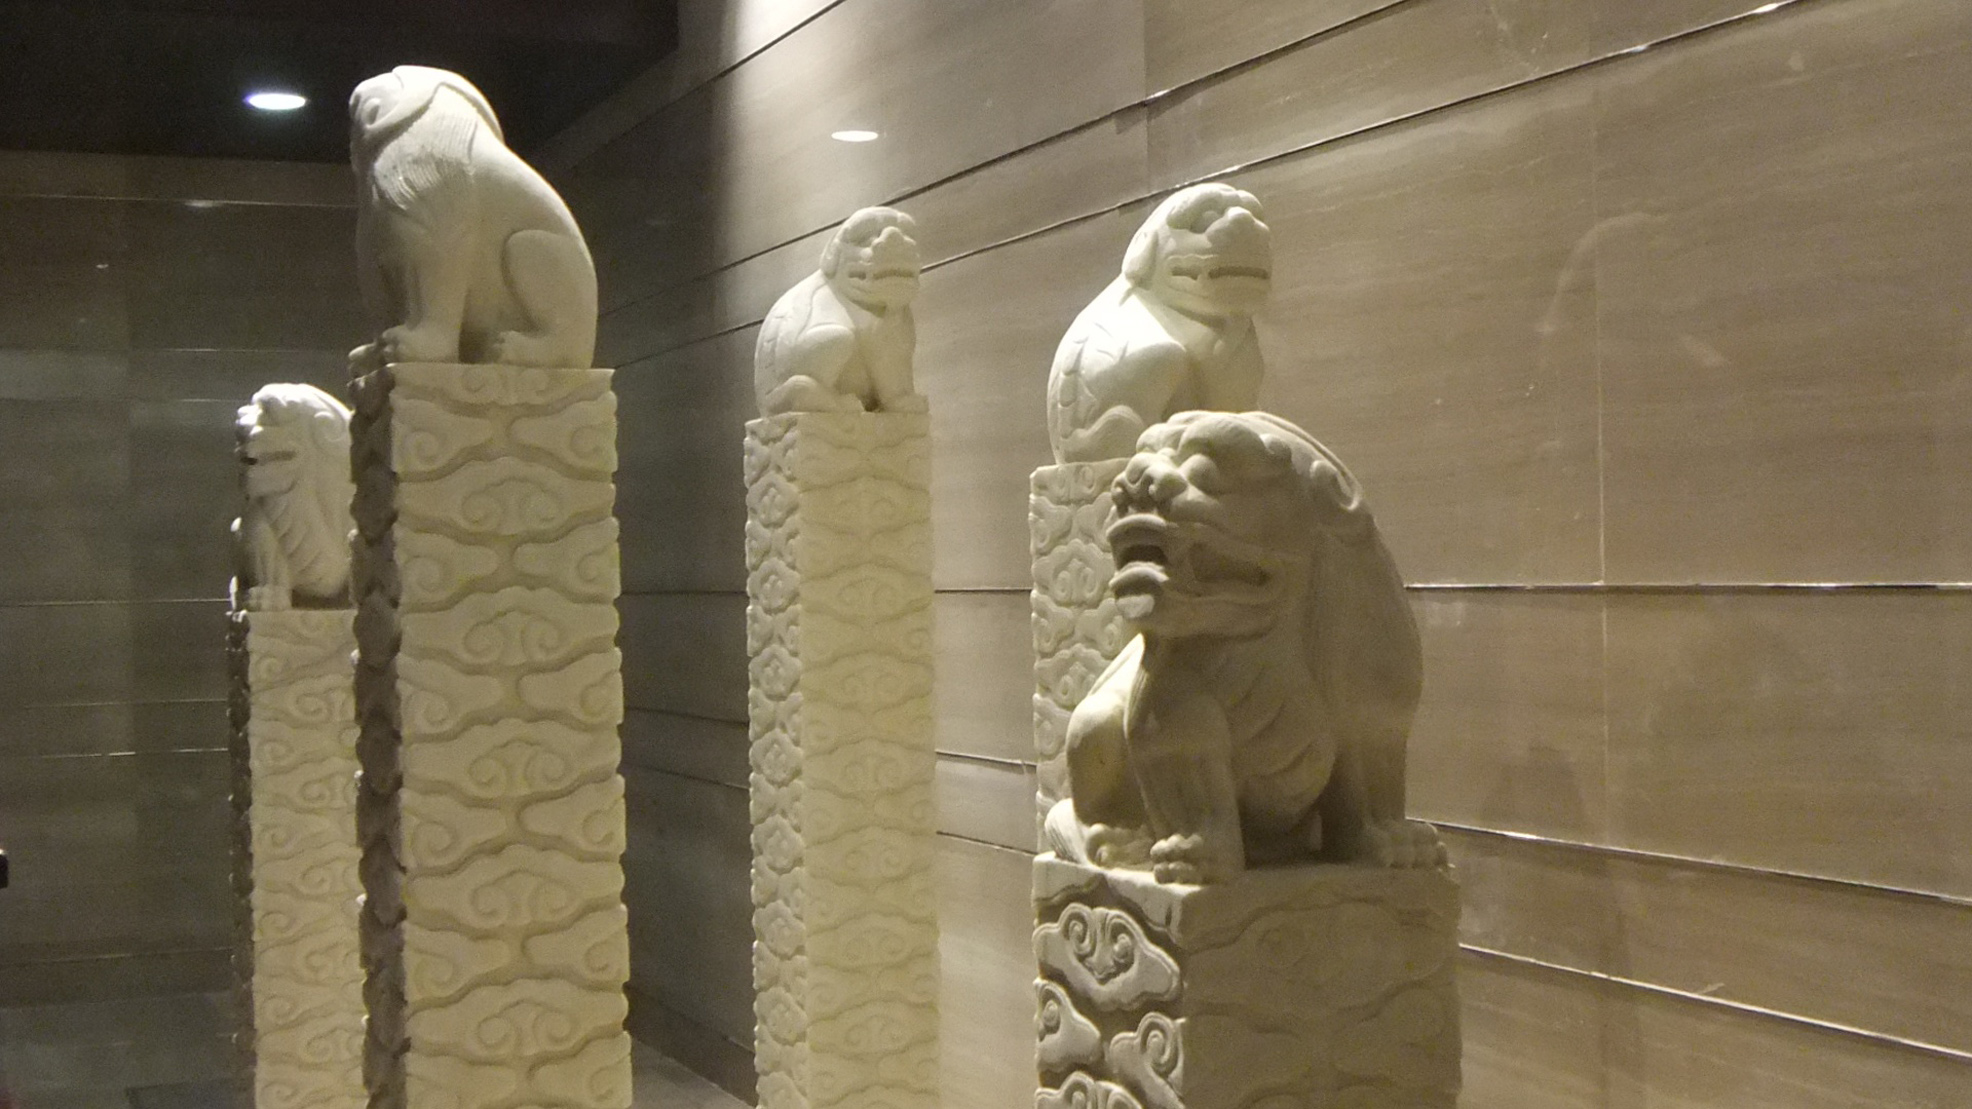
\includegraphics[width=0.3\textwidth]{chap3/32_l}}
    \subfigure[]{
    \label{fig:86_l} %% label for first subfigure
    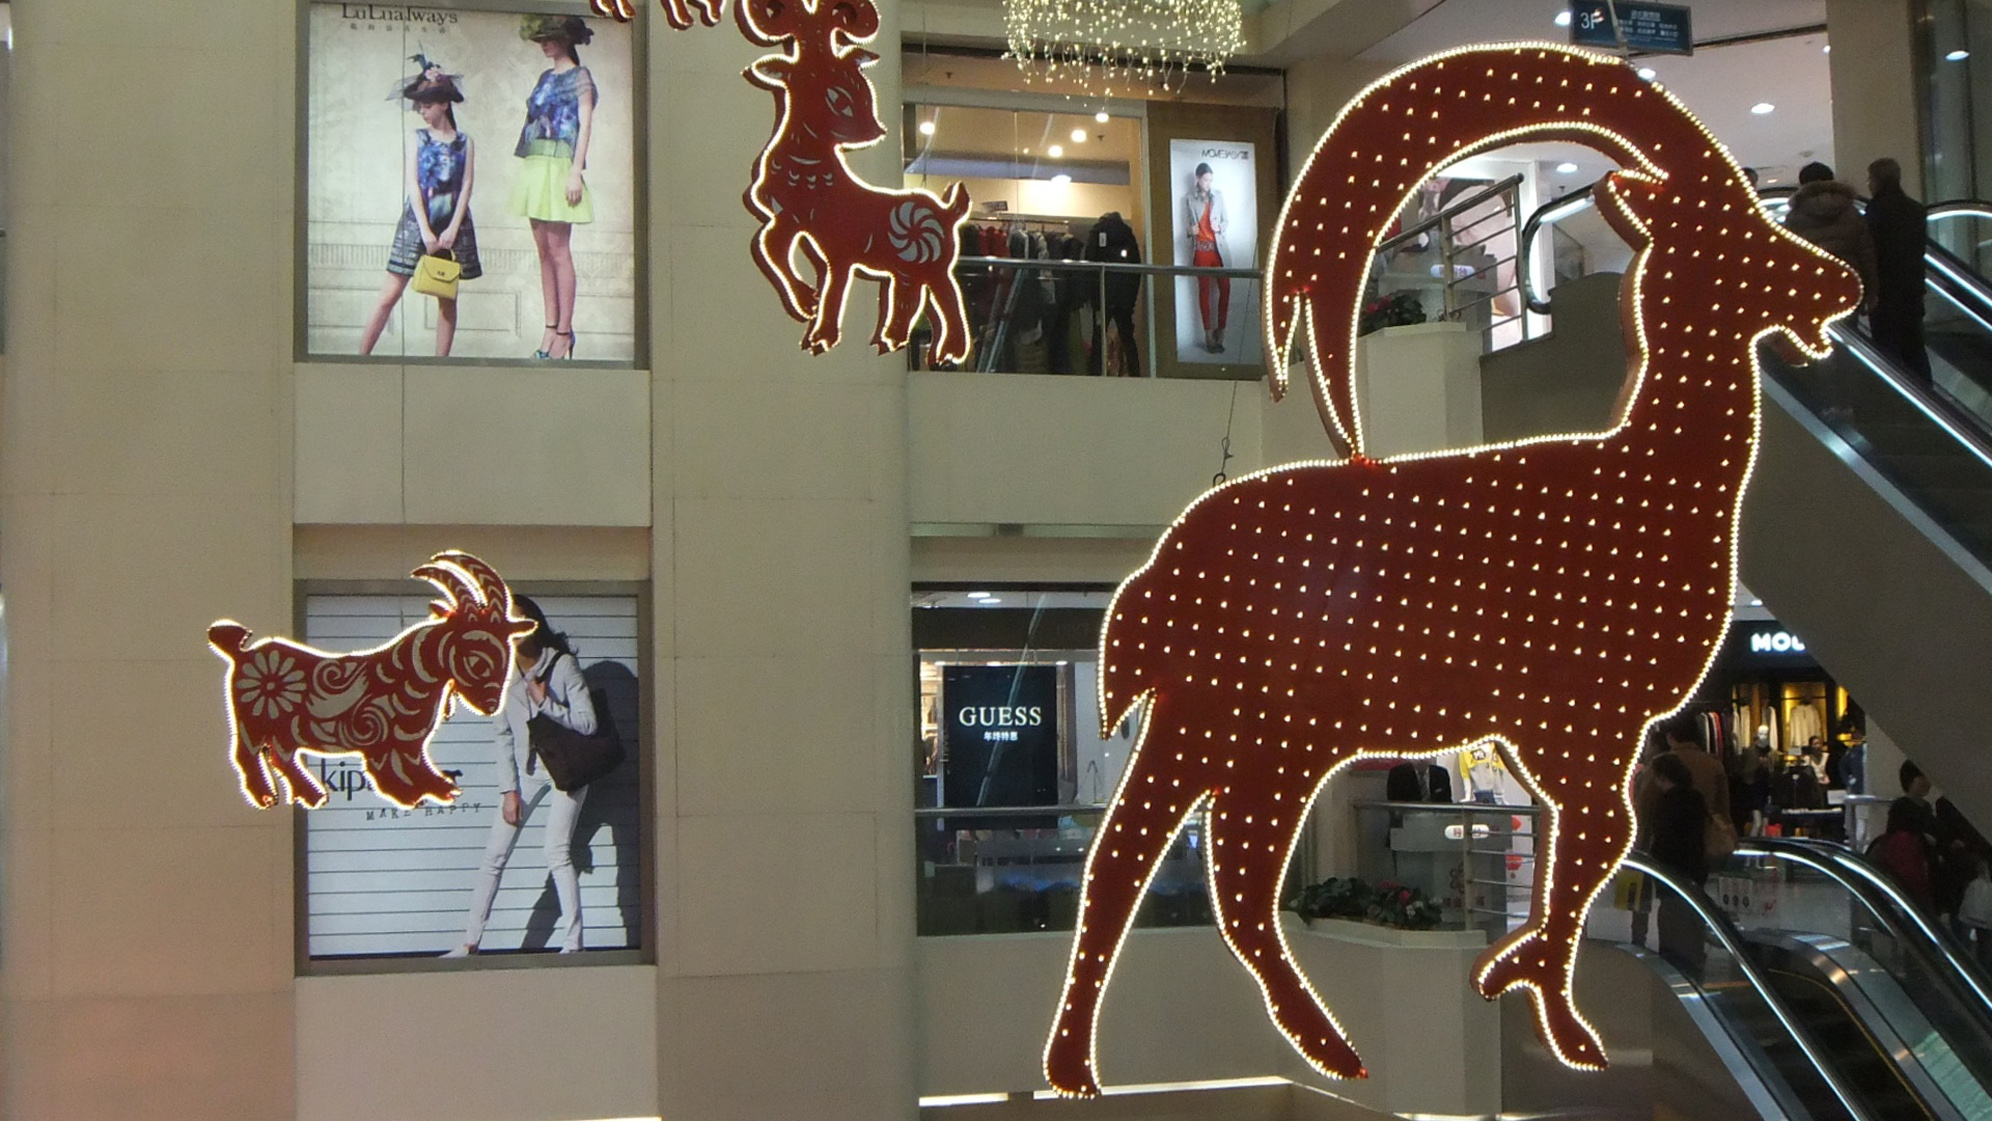
\includegraphics[width=0.3\textwidth]{chap3/86_l}}
  \subfigure[]{
    \label{fig:104_l} %% label for second subfigure
    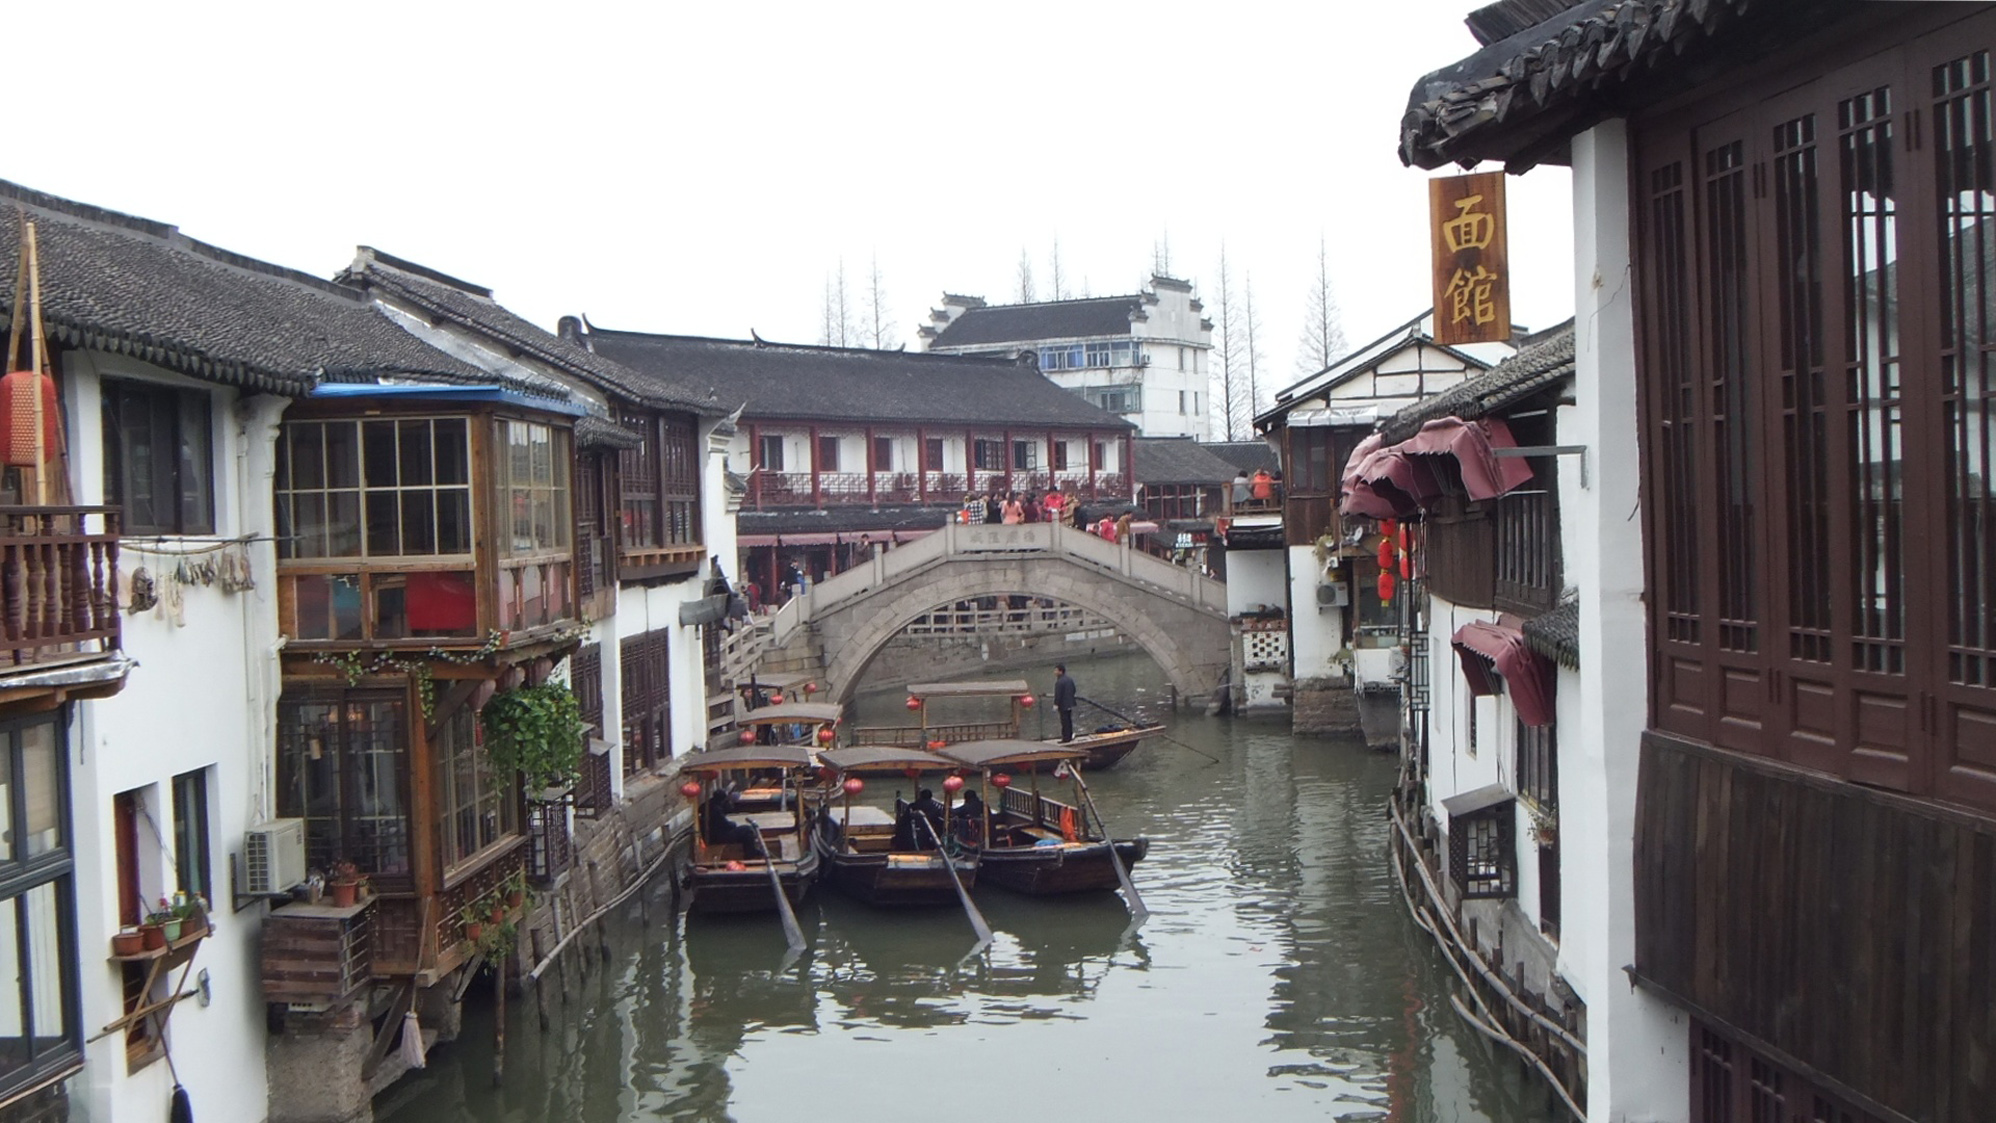
\includegraphics[width=0.3\textwidth]{chap3/104_l}}
  \bicaption[fig:origImageforexpriment]{(a)-(k)为选取的11幅图像的左图}{(a)-(k)为选取的11幅图像的左图}{Fig}{The 11 original left images we choosed}
\end{figure}

针对每幅图像,我们采用下面的方法对图像进行视差调整:

第一,将图像在宽和高的方向放大1.2倍,扩展出用于移轴的区域;

第二,通过移轴,使图像达到最舒适的区域$A_0$。该区域是由几名有3D经验的观看者共同确定。

第三,设当前的位置$A_0$为初始位置,分别从正负两个方向进行视差调整(正表示左右图向相反方向运动,结果是相对入屏;负表示左右图相向而行,结果相对出屏),根据多次的实验经验发现,当视差调整的步长设定为11pixel(对应视差角22 arcmin)时,相邻图像的质量差异明显。

第四,分别在移轴值为0,-11,11,22,-22,34,-34处记录当前图像。这样每幅图像可以变换出7幅相同内容但不同质量的图像。图\ref{fig:shiftaxis}给出了移轴值为正时移轴过程示意图。

第五,为了\ref{sec:densitymap}立体图像分层表示的方便,利用Zhou\parencite{zhou2015depth}的算法获得了所有图像的视差图。

通过以上方法,我们创建了用于眼动实验的立体图像库(7*11幅立体图像和相应的视差图)
\begin{figure}[!htp]
  \centering
  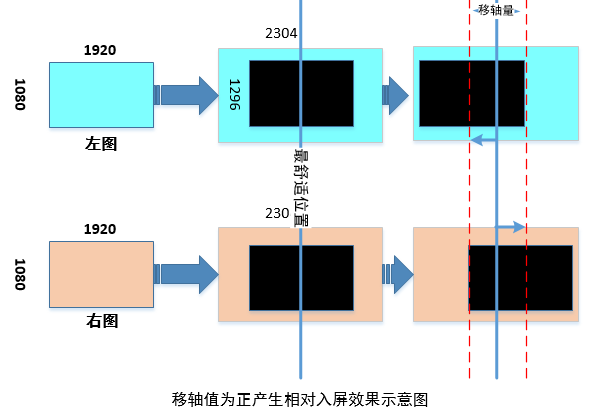
\includegraphics[width=0.75\textwidth]{chap3/shiftaxis}
  \bicaption[fig:shiftaxis]{左右图向相反方向移动,移轴值为正的视差调整示意图}{左右图向相反方向移动,移轴值为正的视差调整示意图}{Fig}{The example when shift value is positive}
\end{figure}
\subsection{眼动数据采集系统的需求分析}
\label{sec:systemrequirement}
眼动数据采集系统的开发依赖于本文的研究目的,同时也要兼顾以后的可能扩展。当前的眼动仪自带处理软件是针对2D场景设计的。本课题的研究对象是立体图像,所以眼动数据采集系统要处理3D图像的场景。另一个问题是,眼动仪自带软件并不是针对图像质量评价设计的,其对图像质量评价的方法支持不足,特别是缺少对双刺激等模式的支持,无法满足不同质量评价方式的需求。最后,从眼动仪与眼动数据的利用效率的角度来看,传统的本地化设计是数据远程利用与共享的短板,因此,利用“云”思想,可以将眼动任务的发布与数据的存储设计为在线模式,这样既可以使眼动仪使用更加便捷性,也为眼动数据的共享与使用提供了便利。

\subsection{眼动数据采集系统的设计}
\label{sec:systemdesigner}
基于上述需求,本课题将基于Tobii SDK和Qt,设计新的眼动数据采集系统。在工程实践中,本系统将发布任务与数据存储与本实验室的图像质量测评众包网站\footnote{\url{http://3dvqa.sjtu.edu.cn/3dvqa}}进行了连接。系统在后续的实验中进行了调试使用,各项功能符合系统设计需求。图\ref{fig:eyetrackingdatacollect}给出了眼动数据采集系统的设计概要。
\section{眼动数据采集系统的开发}
\label{sec:eyetrackdatacollection}
\begin{figure}[!htp]
  \centering
  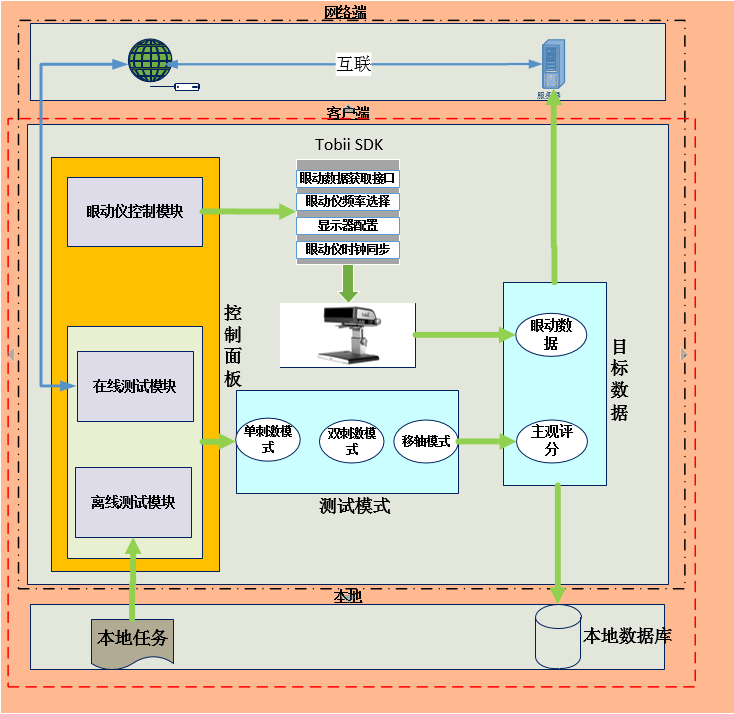
\includegraphics[width=\textwidth]{chap3/eyetrackingdatacollect}
  \bicaption[fig:eyetrackingdatacollect]{眼动数据采集系统设计图}{眼动数据采集系统设计图}{Fig}{The eyetracking data collection system designer map}
\end{figure}

从图\ref{fig:eyetrackingdatacollect}可以看出,眼动数据采集系统从功能上来看分为三个部分:一是眼动数据采集系统的综合控制模块。这部分涉及到眼动仪的正常运行的基本配置,图像格式处理以及测试方法的设定和控制等,是本系统的基本功能部分;二是本地管理模块,主要涉及从本地创建任务以及本地数据的维护和操作;三是与服务器的通信交互模块,主要涉及在线任务的获取与实验数据的远程存储。下面我们将分别对这三个模块进行介绍。

\subsubsection{眼动数据采集系统的主控模块}
\label{sec:controller}
眼动数据的主控制模块的功能包括眼动仪的正常运行控制、图像格式控制以及测试模式控制。

眼动仪的正常运行机制需要四个基本功能的设定。

第一,显示器的配置。本课题采用的眼动仪为Tobii X120眼动仪,它是一种便携式高精度眼动仪,其日常配置并不包括显示器。因此,眼动仪正常运行的第一步是正确地将显示器配置给眼动仪。Tobii SDK提供了配置接口,如图\ref{fig:configuration}所示\parencite{manualuser}。可以看出显示器配置的实质是将显示器左上、右上、左下三个角在以眼动仪正面中心为原点的坐标系UCS中的坐标通过SDK的接口传给眼动仪,这样,眼动仪就可以获取显示器的位置。
\begin{figure}[!htp]
  \centering
  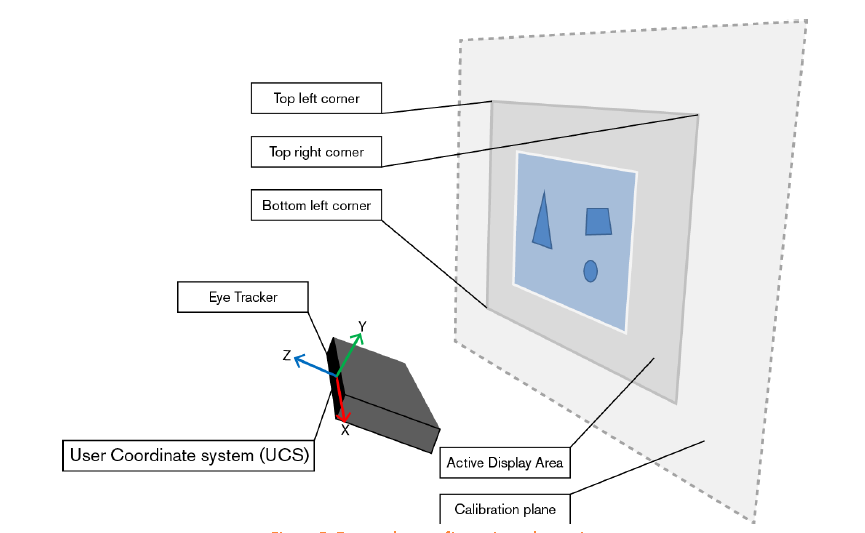
\includegraphics[width=0.75\textwidth]{chap3/configuration}
  \bicaption[fig:configuration]{显示器的配置,需要将显示器的三个角的坐标传给眼动仪}{显示器的配置,需要将显示器的三个角的坐标传给眼动仪\supercite{manualuser}}{Fig}{The configuration procedures for screen to eyetracker\supercite{manualuser} which need transform three corners cordinary of screen to eyetracker}
\end{figure}
\begin{figure}[!htp]
  \centering
  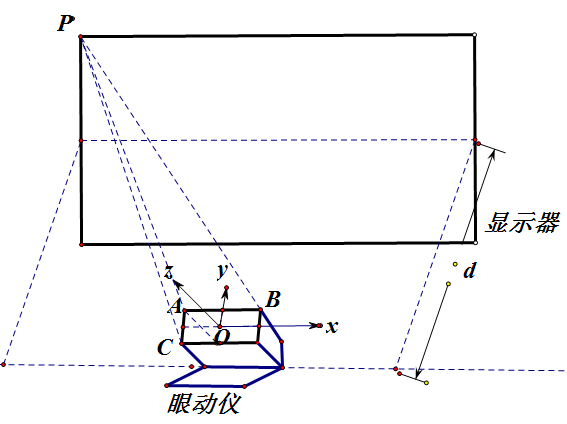
\includegraphics[width=0.7\textwidth]{chap3/eyetrackconfiguration}
  \bicaption[fig:eyetrackconfiguration]{三点距离法求显示器三个角的坐标示意图}{三点距离法求显示器三个角的坐标示意图}{Fig}{The method to obtain the required points }
\end{figure}
为了使配置更加精确,本实验采用了如下方法:首先根据眼动仪表面的几何关系,获取眼动仪左上、左下、右上三个位置的坐标,然后利用激光测距仪分别获取这三个点到显示器上待测的三个点的距离,通过距离公式,我们就能得到显示器相应的三个点的坐标。更具体的,假设$O$为眼动仪正面中心,以$O$为原点建立空间直角坐标系$O-xyz$,根据眼动仪的尺寸可以得到眼动仪正面三个角$A(x_a,y_a,z_a),B(x_b,y_b,z_b),C(x_c,y_c,z_c)$的坐标。利用激光测距仪可以得到这三个点到显示器上待求点$P(x,y,z)$的距离$\left| {\overrightarrow {PA} } \right|,\left| {\overrightarrow {PB} } \right|,\left| {\overrightarrow {PC} } \right|$。利用这三个距离得到三个方程,便可求得点$P$坐标。为了是结果更加准确,激光测距要进行多次,然后取均值以减小误差。

第二, 采样频率的选择。由于眼动仪在不同的采样率下精度不同,所以要先选择采样率。Tobii X120支持两种采样频率——60Hz与120Hz。60Hz的精度更高,这里我们选用60Hz。Tobii SDK提供了设置采样率的接口。

第三,时钟同步。眼动仪与所连接的计算机都内置了时钟,二者会随着工作时间的增加产生延迟。因此,需要每隔一段时间进行时钟同步调整。Tobii SDK提供了相应的调整接口和算法。

第四,2D校正。系统的偏差不可避免,且在不同的被试者测试时表现也有差异,因此,对于每个被试者来说,测试的第一步就是要进行校正,否则所采数据在精度上得不到保障。Tobii SDK自带了2点法、5点法、9点法(屏幕上预先设置目标的个数)等三种方法,并支持点的增删,应用Qt的相关技术,本系统实现了5点法校正。

除了以上四个基本功能,本系统自己开发了两个功能:一是眼睛实时追踪状态显示功能,即开辟了一个单独线程,通过Tobii SDK返回的眼睛数据,可以实时查看眼睛是否被眼动仪正确捕捉,此功能在较长时间的测试中的作用很大;另一个是校正辅助程序,某些用户在校正过程中校正效果始终无法达到可接受的水平,一般情况下,这是由坐姿不正确引起的,这个功能通过预先在屏幕上显示一些点,让被试者去看屏幕,此时会实时显示用户的注视位置与预设点的位置关系,帮助用户进行坐姿调整。

主控模块的第二个功能是对3D图像格式的处理,系统支持3种格式的图像输入:左右图直接输入、合成的左右图以及合成的上下图。用户需要在任务设定阶段指定要输入图像的格式。对于在线任务,我们与服务器端约定了只能发布左右原图的任务,测试时系统会将图像处理成3D电视可以直接播放的格式。

主控模块另一个主要功能是测试模式控制,系统共实现了三种模式:单刺激模式、双刺激模式、移轴模式。

单刺激模式对应于图像的单刺激质量评价方法,即一张图对应一次测试过程,图像播放特定的时长(一般为10s),这段时间采集眼动数据。在开始下次测试前,间隔3s让被试者休息。另外,根据眼动数据采集完是否对图像进行评分,本系统还支持有任务与无任务两种模式,其中有任务模式下评分采用单刺激图像质量评价的5分制,而无任务测试则只有眼动数据,不进行图像评分。本文的实验\ref{sec:stereoscopicimageeyetrackdatacollecting}就是采用了有任务的眼动实验这种模式。

双刺激模式对应于图像的双刺激比较评价方法,即两张图对应一次测试过程,两图各播放10s,期间间隔3s用以消弱前图对后图的影响。该模式也实现了有任务与无任务两种模式,有任务的评分实现了PairWise比较的5分制(-2,-1,0,1,2分别表示前图比后图差的多、稍差、差不多、较好、好)。

移轴模式并不对应于任何图像质量评价方法,主要是为了研究立体图像的视差变化对图像质量的影响提出的。移轴的方法如图\ref{fig:shiftaxis}所示,本系统在实现时以2个像素作为移轴步长来调整视差。正是通过这个模式的检验,使得我们意识到当移轴步长在10个像素左右时,图像质量的差异比较明显,也据此创建了立体图像库。

以上是主控模块的主要功能,当然,主控模块还包括了与其他两个模块的交互,以及信息管理等,在介绍相应模块时再来叙述。
\begin{figure}[t]
  \centering
  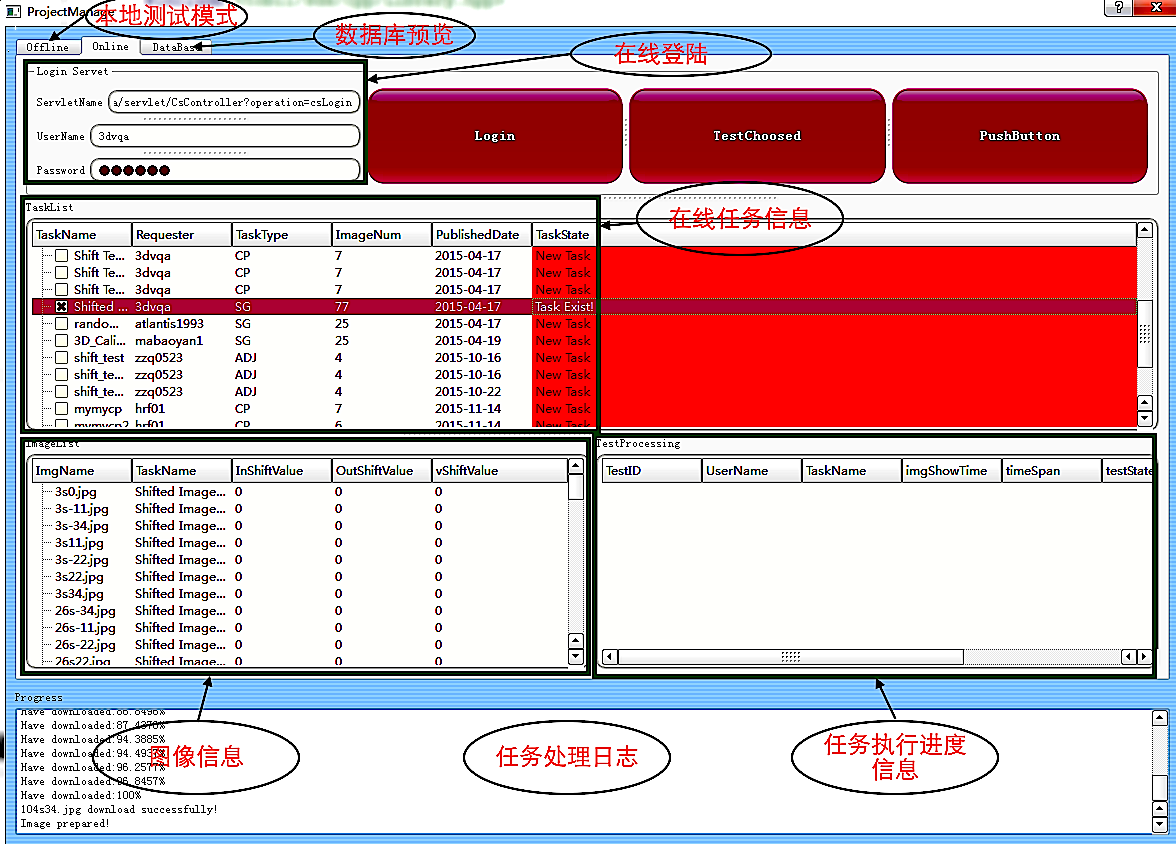
\includegraphics[width=\textwidth]{chap3/eyetrackingdatasystem}
  \bicaption[fig:eyetrackingdatasystem]{眼动数据收集系统在线测试部分示意图,包括登陆信息、当前可测试任务信息、当前正在测试任务图像信息、当前测试任务进度信息以及处理日志信息}{眼动数据收集系统在线测试部分示意图,包括登陆信息、当前可测试任务信息、当前正在测试任务图像信息、当前测试任务进度信息以及处理日志信息}{Fig}{The online part of eyetracking data collecting system,which contains login info,task info,image info,test info and log info}
\end{figure}
\subsubsection{眼动数据采集系统的本地管理模块}
\label{sec:local}
眼动数据采集系统的本地管理模块包括:一是本地任务的创建,主要是从本地的图像库直接创建任务,无需与网站交互;二是在线任务的本地化管理,当从Web服务器获取任务后,由于多个被试者会测试同一个任务,所以其所占资源可以共享,本地化模块将负责这些资源的管理与调配;三是本地数据库的管理,本地或在线任务在测试时产生的所有信息都需要保存在本地数据库,以备后续使用。

第一,本地任务的创建。本地任务的创建首先是存在性检验,任务创建时检验任务是否存在,用户测试时检验用户是否存在,测试进行时检验是否已进行过测试或者用户的当前测试进度等。其次,是任务类型选择和参数设置,前面提到的三种模式和相应的参数(如播放时间,休息时间,移轴范围等)在这里设定,最后,前述所有的改动或新信息都要与本地数据库交互验证更新。

第二,对在线任务管理。在与服务器交互获取用于测试的任务后,这些任务信息会被保存,相关信息进入数据库。当其他被试者进行相同任务测试时,此时无需再去请求任务,只要使用本地备份任务即可,图\ref{fig:eyetrackingdatasystem}给出了在线测试任务的管理系统。

第三,对本地数据库的管理。本地数据库采用了sqlite3,数据库的操作基于Qt的数据库操作模块QSql进行的。几乎任务的每一个环节都涉及到数据库的操作。包括任务创建时的任务信息、图像信息、任务状态、被试者加入时的用户信息、眼动数据和主观评分产生时的记录信息以及上传状态等。为了更友好的管理本地数据库,我们还开发了数据库的预览程序,可以随时查看任务、用户、数据的各种信息。
\begin{figure}[!htp]
  \centering
  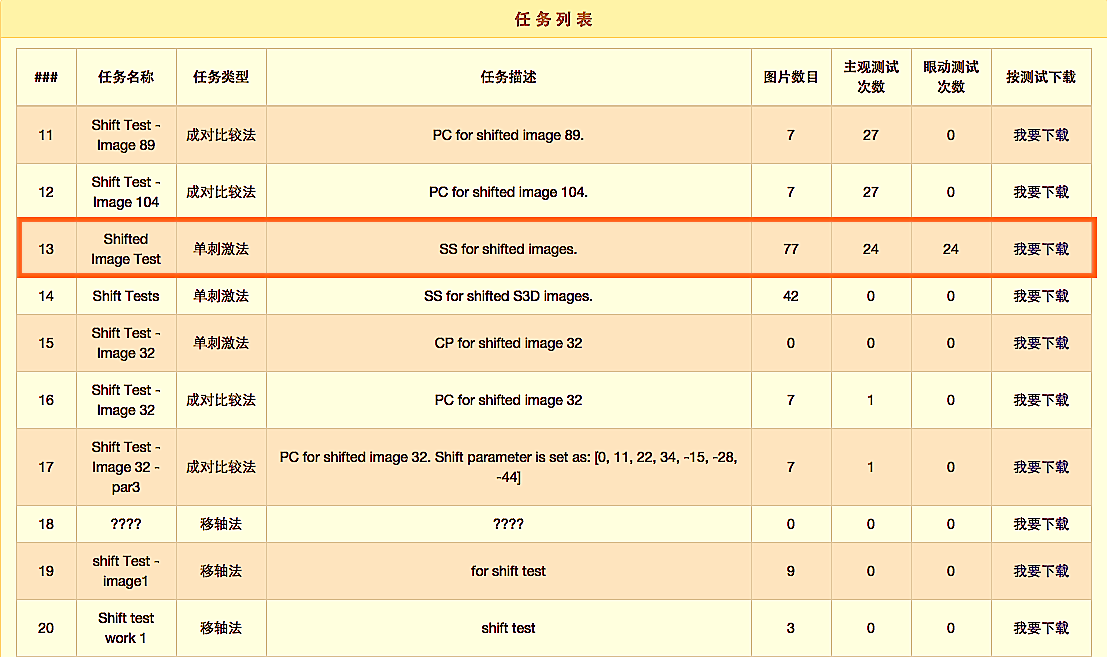
\includegraphics[width=0.75\textwidth]{chap3/eyetrackdata}
  \bicaption[fig:eyetrackdata]{眼动数据收集系统在线交互模块数据上传部分,图中红色框内是本实验眼动数据收集结果}{眼动数据收集系统在线交互模块数据上传部分,图中红色框内是本实验眼动数据收集结果}{Fig}{The online part of eyetracking data collecting system,our results were showed in the red box}
\end{figure}
\subsubsection{眼动数据采集系统的在线交互模块}
\label{sec:online}
前面我们提到,任务发布与数据存储在线化有利于眼动仪与眼动数据的应用。数据采集系统的在线交互模块是与服务器通信过程的集合。主要分为任务获取与数据上传两部分。

任务获取包括任务请求、图像下载、本地临时任务创建、本地数据库更新等过程。任务请求过程的通信方式为xml文件交换,其结构化的表述能力很适合表达任务信息。图像的下载采用了多线程的方法实现,以利于图像下载时其他功能的正常执行。任务获取的过程是整体实现的,会在本地创建一个临时任务方便管理,任务的管理是通过操作数据库实现的。

数据的上传包括眼动数据与主观评分数据(如果有任务的话)的上传,数据的上传在每一幅图像测试完成后都会执行。上传成功的数据会将本地数据库中上传的状态更新为成功,否则,程序要尝试重新上传或者在网络等外界环境正常时人工上传,图\ref{fig:eyetrackdata}给出了眼动数据收集系统在线收集结果。

眼动数据采集系统经过调试与验证,最后在立体图像眼动数据实验中表现很稳定。
\section{眼动实验的设计与实施}
\label{sec:conductexperiment}
本实验旨在获取观看立体图像时的眼动数据,为了保证获取的实验数据有效性与准确性,需要对实验的各个环节进行设计。除了实验场景按照ITU-R BT.500-12的标准执行之外,还要对实验者自身的素质进行检测,本文将设计一个立体视敏度检测实验来检验每个被试者的立体视觉是否正常,然后剔除掉检测结果为“立体盲”的用户。由于眼动仪本身只有2D校正过程,为了提高3D测试的精度,本文还将设计了一个离线的3D校正实验,实验数据用来测量每个被试者的系统性误差,用于\ref{sec:calibraiton}的校正过程。最后,本文将给出观看立体图像时眼动数据的采集过程。
\subsection{实验设备}
\label{sec:eyetrackerandTV}
本实验采用了一台47英寸的LG 3D显示器(如图\ref{fig:3dtv}),其分辨率为1920x1080,宽高为104.1x58.5cm,支持左右、上下、红青等3D格式。实验采用的眼动仪为Tobii X120眼动仪(如图\ref{fig:tobii}),采样率可选60Hz与120Hz,具有100ms的追踪补偿能力,最大扫视角度为${35^ \circ }$,最大头动速度为35cm/s ,在60Hz的采样频率下允许44x22x30cm(宽x高x深度)的头动范围,120Hz下的头动范围为33x22x30cm(宽x高x深度)。实验采用的控制平台是\ref{sec:systemdesigner}开发的眼动数据采集系统。
\begin{figure}
  \centering
  \subfigure[3D 电视]{
    \label{fig:3dtv} %% label for first subfigure
    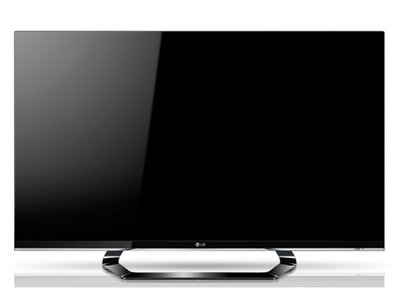
\includegraphics[width=0.3\textwidth]{chap3/3dtv}}
  \subfigure[Tobii 眼动仪]{
    \label{fig:tobii} %% label for second subfigure
    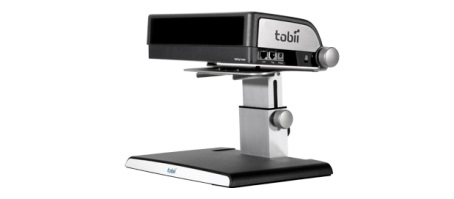
\includegraphics[width=0.5\textwidth]{chap3/tobii}}
  \bicaption[fig:apparatus]{眼动实验设备}{眼动实验设备}{Fig}{Eyetracking experiment Apparatus.}
\end{figure}

\subsection{被试者(实验参与者)}
\label{sec:subjects}
参与实验的27名初选被试者均来自中国计量学院信息工程学院\footnote{\url{http://xxgcxy.cjlu.edu.cn/}}的学生,所有人有3D电影经验但均非专业研究人员。其中男生17人,女生10,年龄介于$21 \sim 27岁$(均值为23.52,标准差为1.67),被试者中存在近视情况,但校正视力均正常,无眼疾被试者。样例视频(功夫熊猫3D选段)观看过程未见异常。
\subsection{立体视敏度检验与主眼主观确认实验}
\label{sec:stereoacuitytest}
立体视敏度检验实验是为了测量被试者的立体感是否正常。 ITU-R  BT.1438\parencite{recommendation1438}给出了相关的测试图像(图\ref{fig:vt04})与测试方法。
\begin{figure}[ht]
  \centering
  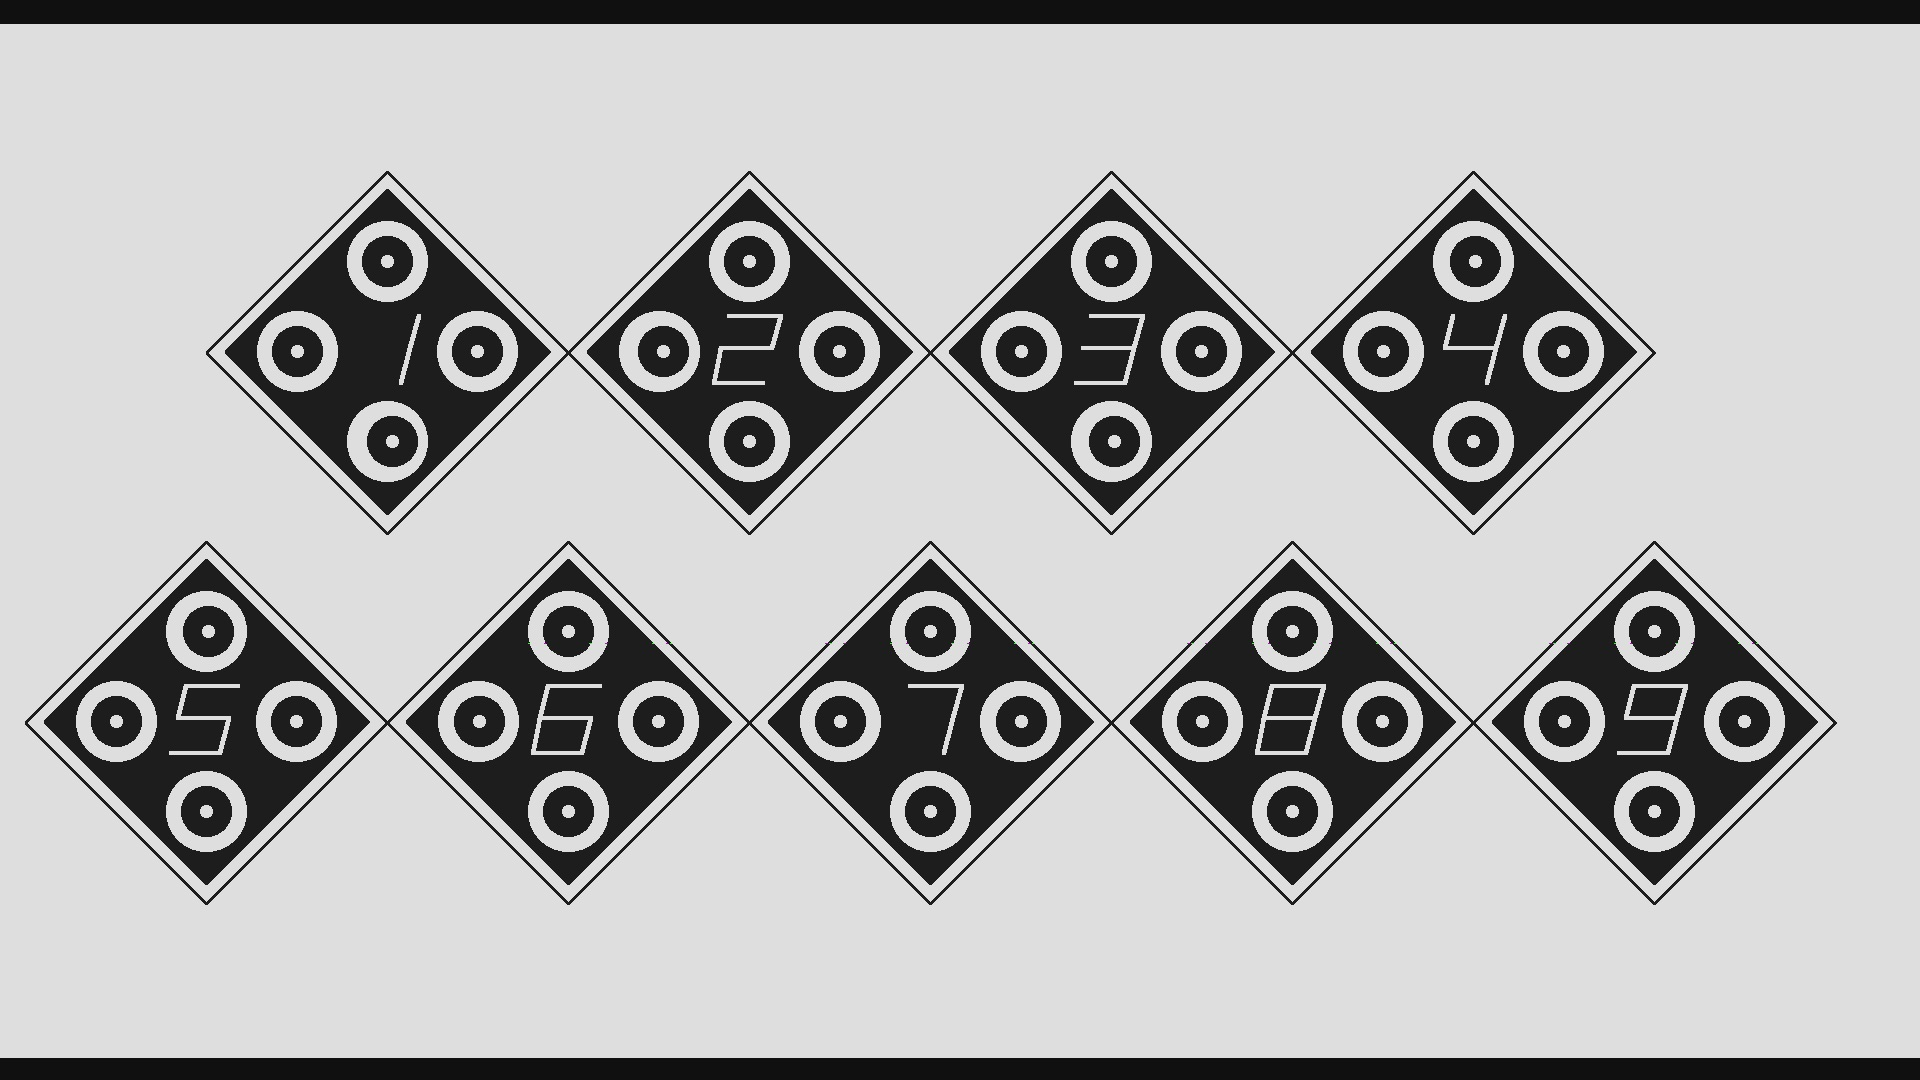
\includegraphics[width=0.75\textwidth]{chap3/vt04}
  \bicaption[fig:vt04]{立体视敏度检验图片对的左图,每四个圆圈一组,其中有一个存在轻微视差,从第一组到第九组,视差逐步减小}{立体视敏度检验图片对的左图,每四个圆圈一组,其中有一个存在轻微视差,从第一组到第九组,视差逐步减小}{Fig}{The image for testing stereo acurity,there is tiny disparity in each group and the disparity decrease from the first group to the last}
\end{figure}
图为测试图像的左图,其中共包含编号从$1 \sim 9$的9组圈集,每组里面包含4个小圆圈,其中一个与相应右图上得圆圈存在轻微的视差,其余的均与相应右图的圆圈无视差,这样,立体视敏度正常的人就可以看到其中一个圈与其他圈不在同一个平面上。各组存在的视差从第一组开始逐步降低,直到第9组时视差为0。所以从1到9,立体感获取难度逐步增加。具体的,各组存在视差的圆圈的位置与具体视差角(从3倍屏高处看)的大小(单位为 arc sec)如表\ref{tab:correctanswer}所示。
\begin{table}[]
\centering
\caption{测试图像中各组存在视差的点的位置与视差值}
\label{tab:correctanswer}
\begin{tabular}{|c|c|c|}
\hline
\multirow{2}{*}{Test No.} & \multirow{2}{*}{Correct answers} & \multirow{2}{*}{Angle of stereopsis at 3 H(")} \\
                          &                                  &                                                \\ \hline
1                         & Bottom                           & 480                                            \\ \hline
2                         & Left                             & 420                                            \\ \hline
3                         & Bottom                           & 360                                            \\ \hline
4                         & Top                              & 300                                            \\ \hline
5                         & Top                              & 240                                            \\ \hline
6                         & Left                             & 180                                            \\ \hline
7                         & Right                            & 120                                            \\ \hline
8                         & Left                             & 60                                             \\ \hline
9                         & \_                               & 0                                              \\ \hline
\end{tabular}
\end{table}
被试者被要求从第一组开始逐组说出不在同一平面的圆圈的位置。这里对所有被试者的结果做了统计,如图\ref{fig:stereoacurityresult}所示。
\begin{figure}[ht]
  \centering
  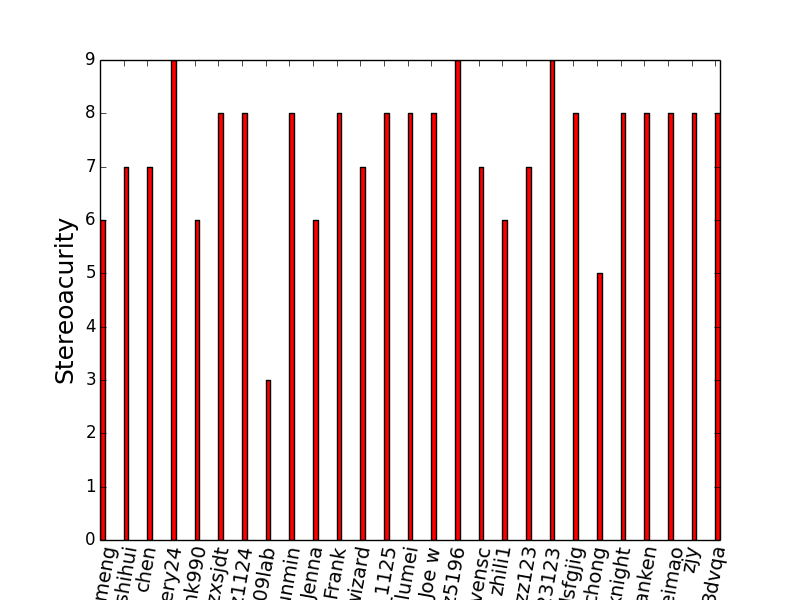
\includegraphics[width=0.7\textwidth]{chap3/stereoacurityresult}
  \bicaption[fig:stereoacurityresult]{所有被试者立体视敏度的结果,纵轴表示该被试者可以看到的最高组号}{所有被试者立体视敏度的结果,纵轴表示该被试者可以看到的最高组号}{Fig}{The result of stereoacurity test, where the y axis represents the highest group one can catch}
\end{figure}
结果显示,昵称为“609lab”的被试者只能看到前三组,所以相对立体视敏度过差,我们拒绝该被试者参与下面的实验。
由于滤波和特征提取时区分了主眼和辅眼的作用,本文在实验开始时都会对被试者进行主眼检测。主眼的测试的方法较简单\footnote{\url{http://academy.fengniao.com/299/2995808.html}},这里不再赘述,实验中所有被试的主眼情况如图\ref{fig:maineye}所示。
\begin{figure}[!htp]
  \centering
  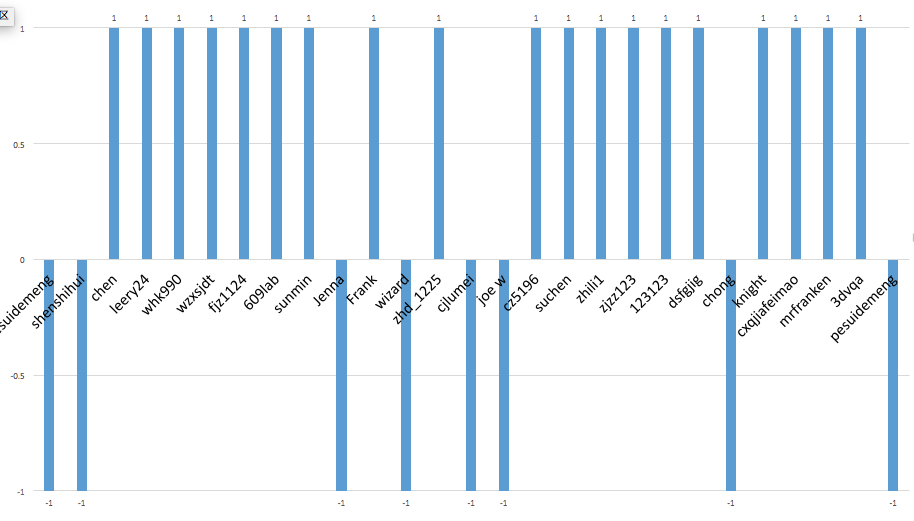
\includegraphics[width=0.7\textwidth]{chap3/maineye}
  \bicaption[fig:maineye]{所有被试的主眼检测情况,-1代表主眼为左眼,+1代表主眼为右眼}{所有被试的主眼检测情况,+1代表主眼为左眼,-1代表主眼为右眼}{Fig}{The main eye for subjects where +1 means the main eye is left eye while -1 is right eye}
\end{figure}
\subsection{3D校正实验}
\label{sec:3dcalibrationexperiment}
校正是处理测量系统自身存在的稳定、持续性误差的主要的手段。对于眼动追踪实验,系统误差主要来自于两个方面,一是实验器械自身的系统偏差与实验环境配置(眼动仪的精度以及眼动仪与显示器的配置)带来的误差;二是被试者自身的系统偏差(不同人眼存在个体差异,因此在同一系统参数下表现也不相同)。眼动仪的2D校正程序会消除这类误差。除此之外,在观看3D素材时,个体之间还存在立体感的差异(如图\ref{fig:stereoacurityresult}),因此往往测量的数据在深度上的表现如图\ref{fig:beforecalibration:a}所示,这就产生了一个立体感的系统偏差。因此,在3D场景下要设置一个3D校正过程。这里采用离线校正的方法——校正过程的系统误差在线下获取并执行。

为了校正深度方向的偏差,首先要让被试者观看预先设置在不同深度平面的不同位置的“目标”,这些目标对应的深度信息已知,然后通过记录的眼动数据可以获取测量深度,这样,可以通过已知深度与测量深度获取系统偏差。这个偏差用来校正后面的立体图像眼动数据。我们设置五个深度平面,其对应的视差(视差角)为 -30, -10, 0, 10, 30  ($ -{0.5345^\circ }, -{0.1782^\circ }, {0^\circ }, {0.1782^\circ }, {0.5346^\circ }$),如图\ref{fig:calibrationpoint}所示。
\begin{figure}[!htp]
  \centering
  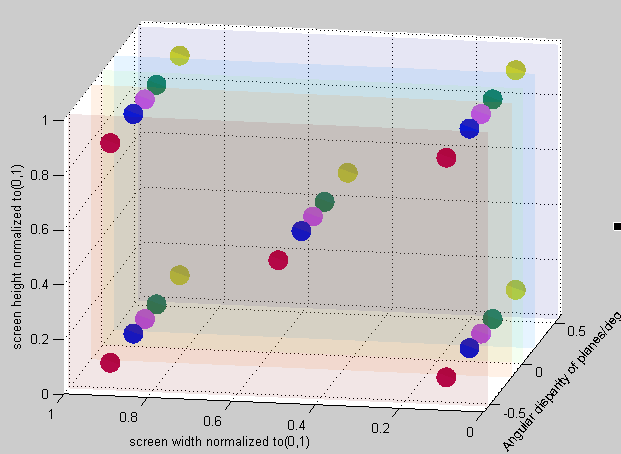
\includegraphics[width=0.6\textwidth]{chap3/calibrationpoint}
  \bicaption[fig:calibrationpoint]{3D校正过程的25个“目标”空间分布图}{3D校正过程的25个“目标”,分别位于视差角为$ -{0.5345^\circ }, -{0.1782^\circ }, {0^\circ }, {0.1782^\circ }, {0.5346^\circ }$的深度平面的(0.1,0.1), (0.1,0.9), (0.5,0.5), (0.9,0.1), (0.9,0.9)处}{Fig}{The 25 targets for 3D calibration located at point (0.1,0.1), (0.1,0.9), (0.5,0.5), (0.9,0.1), (0.9,0.9) in five depth planes where disparity angular is $ -{0.5345^\circ }, -{0.1782^\circ }, {0^\circ }, {0.1782^\circ }, {0.5346^\circ }$}
\end{figure}
由于人眼对同一种颜色的目标的立体感并不强\parencite{holliman2007application},因此,传统的同色点图在这里并不适用。本文实验中采用“点”内被噪化处理过的“点图”,即图\ref{fig:calibrationpoint}中的目标实际应用时内部存在多种随机的颜色。另外,目标的直径也是我们考虑的一个重要因素,我们尝试了直径分别为10,14,16,18,22像素等五个级别的点图,发现直径为10,14的目标过小,每次需要较长的聚焦时间,而直径为22时,目标过大,引入的误差相对就大。所以,综合考虑使用了直径为18像素的目标。

实验的基本流程是:
\begin{itemize}[noitemsep,topsep=0pt,parsep=0pt,partopsep=0pt]
\item 首先,眼动仪开启,准备记录数据,在辅助程序下调整个人坐姿,使双眼稳定的被眼动仪捕捉;
\item 从25个目标中随机选一个,开始播放,于此同时记录眼动数据,时间持续2s,停止播放与数据记录;
\item 由于25个目标的深度有别,为了防止上一个目标对下一个目标的追踪形成干扰,此时黑屏1s,给人眼一段缓冲时间;
\item 轮流执行上面三步,直到25点播放完毕。
\end{itemize}

实验开始时,首先给被试者介绍实验目的与被试者应有的反应,然后按照前面的流程进行一次训练(结果不计),在被试者熟悉流程后开始正式实验。最终,我们获取了24名被试者的3D校正眼动数据(有两名同学的眼睛无法被眼动仪正常的捕捉到,因此,未能参加实验)。
\subsection{立体图像的眼动数据采集实验}
\label{sec:stereoscopicimageeyetrackdatacollecting}
经过\ref{sec:stereoacuitytest}和\ref{sec:3dcalibrationexperiment}的筛选和建议之后,24名被试者参加了立体图像的眼动实验。立体图像的眼动实验是有任务的眼动数据采集实验,即我们将眼动数据采集与图像单刺激质量评价进行了结合,在观看图像时采集数据,观看结束时对图像进行评分。具体来说,一次实验的具体过程可以描述如下:
\begin{itemize}[noitemsep,topsep=0pt,parsep=0pt,partopsep=0pt]
\item 首先,眼动仪开启,准备记录数据,在辅助程序下调整个人坐姿,使双眼稳定的被眼动仪捕捉;
\item 从77幅图像中随机选取一张开始播放,于此同时记录眼动数据,时间持续10s,10s后停止播放与数据记录,屏幕变黑;
\item 此时提示被试者对图像进行评分,评分准则为ITU-R BT.500-11\parencite{recommendation2002500}标准的5分制,1分表示差,2分表示较差,3分表示一般,4分表示良好,5分表示优秀;
\item 轮流执行上面三步。
\end{itemize}

实验开始时,被试者首先要被训练,在眼动数据采集方面,需要给用户强调的是,以最自然的方式观看图像内容,无需刻意地只注视图像内的某些区域。在主观评分方面,需要先展示一些不同质量的样例图片,使被试者有估计图像质量的能力。另外,实验时由于时间太长,立体图像的观看容易引起视觉疲劳,因此,原则上每10幅图像被试者要休息一次。除此之外,为了防止3D图像观看过程中引起不适,被试者可以随时要求中止或中断实验(实际中并未发生)。最后,实验执行者需要经常在监视器内查看被试者的眼睛是否正在被正常捕捉,及时调整被试者坐姿,防止实验结果无效。实验最终获取了24名被试者对77幅图像的眼动数据与单刺激主观评分,如图\ref{fig:eyetrackdata}所示。数据的处理将在第\ref{chap:dataprocess}章进行。
\section{总结}
\label{sec:conclusionchapter3}
本章我们主要做了数据准备工作,包括创建了立体图像库与眼动数据库。

立体图像库包含了77幅图像,这些图像是由11幅图像利用移轴方法调整视差创建的。在图像选取的过程中,我们主要考虑了内容的代表性、深度的分布、深度范围等因素,同时也考虑了图像的显著性区域的多寡。基于图像内容在不同的景深下其质量不同这一事实,我们将每幅图像从质量最好的初始位置进行了7种变换,其调整步长分别为$\pm 11, \pm 22, \pm 34$pixel,这种方法在保证了图像内容几乎不变的情况下使图像的质量产生差异。最后,为了后续应用方便,我们还获取了对应每幅图像的视差图。

眼动数据库的实现除了依赖立体图像库之外,还依赖于眼动数据采集系统和眼动实验。

由于测试的个性化需求,我们首先开发了眼动数据采集系统。系统首先从眼动仪的正常运行机制开始,基于Tobii SDK 完成了显示器的配置、采样率调整、2D-5点法校正以及眼动仪与计算机的时钟同步调整机制等。其次针对3D图像的多种格式,系统开发了图像格式兼容机制,使其可以灵活处理不同格式的立体图像。再次,系统在采集模式上与图像主观评价方法相对应,开发了单刺激、双刺激测试模式。为了研究视差变化对图像质量影响,这里还增加了移轴模式。最后,系统还具有在线与本地发布任务和数据存储的功能。在任务与数据管理方面,系统基于Qt进行了数据库创建与应用,并设置了多重存在性检验机制与反馈机制,增强了系统的可用性。系统在调试与检测后,在实验中表现的很稳定。

眼动实验的设计是本章的重点,为了提高测量的准确性与精度,本文在介绍了相应的实验设施和被试者的基本信息之外,重点介绍了眼动实验的三部分。第一,立体视敏度检验。本实验利用了ITU-R BT.1438的方法测试了27名被试者的相对立体视敏度,最终确认了26名被试者可以继续实验,同时我们也测试了所有被试者的主眼。第二,3D校正实验。本实验是针对3D场景的深度特征提出的,实验的目的是获取预设深度目标的眼动数据,这些数据将在第四章用于计算被试者的系统误差。同时,本实验执行过程中,发现两名被试者的眼睛无法被眼动仪追踪,这也为后续实验节约了时间成本。第三,立体图像眼动实验,实验严格执行了“实验说明——样例训练——正式实验”的步骤,保证了实验测试过程的严谨。

本章最后获取的立体图像—眼动数据库(SIED)包括:77幅立体图像与相应视差图、24位被试者的立体视敏度检验结果和主眼信息、24位被试者观看3D校正目标的眼动数据(24*25组数据),24位被试者观看立体图像时的眼动数据(24*77组数据)。这些数据构成了后续工作的基础。


%# -*- coding: utf-8-unix -*-
\chapter{主观评价与眼动实验数据的处理}
\label{chap:dataprocess}
通过第\ref{chap:databaseconstruction}章的实验,我们得到了两部分数据,一是主观评分数据,二是眼动数据。下面我们分别对这两种数据集进行预处理。

\section{主观评分的处理}
\label{sec:subjectscore}
立体图像的主观评分是在眼动实验\ref{sec:stereoscopicimageeyetrackdatacollecting}中获取的,每幅图像播放10s,获取眼动数据后,眼动仪停止记录,被试将对刚才看到的图像进行评分,整个过程相当于单刺激主观评分。评分区间为1-5分,分别表示图像质量差、较差、一般、良好、优秀等五个等级。本节将首先对数据进行异常值剔除,然后通过保留的数据求对应于各幅图像的MOS值。
\subsection{主观评分异常值检测与剔除}
\label{sec:dropsinglesubjecterrorvalue}
我们的实验被试共记24人,每个人都对77副图像进行了主观评分,为了保证评分的可信度,我们需要做评分的异常值检测。
这里采用ITU-R BT.500-11\parencite{recommendation2002500}标准中针对“单刺激连续测试方法”的异常值检测算法。

第一,确定针对一幅立体图像的评分是否属于正态分布,即对一副图像的评分做${\beta _2}$检验,也称为求Kurtosis系数\parencite{goldmann2010comprehensive}。Kurtosis系数在数学上可以定义为随机变量四阶中心矩和方差平方的比值:
\begin{equation}
kurtosis = \frac{{\sum\nolimits_{i = 1}^N {{{({Y_i} - \overline Y )}^4}} }}{{(N - 1){s^4}}}
\end{equation}
\begin{figure}[htbp]
  \centering
  \begin{minipage}[b]{0.73\textwidth}
    \captionstyle{\centering}
    \centering
    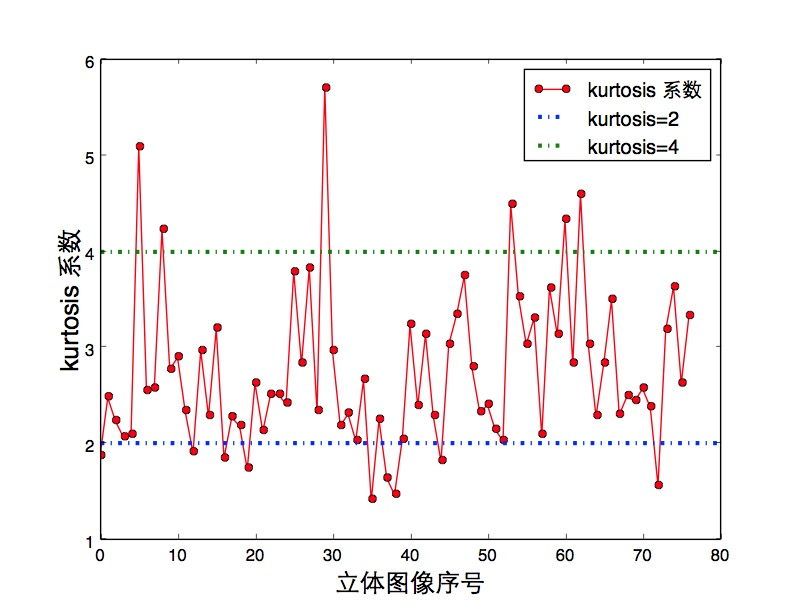
\includegraphics[width=\textwidth]{chap4/kurtosis}
    \bicaption[fig:kurtosis:a]{77幅图像对应的Kurtosis 系数以及正态分布的临界值2,4}{77幅图像对应的Kurtosis 系数以及正态分布的临界值2,4}{Fig}{Kurtosis coeficients of 77 stereoscopic image}
  \end{minipage} %  
  \hfill
  \begin{minipage}[b]{0.74\textwidth}
    \captionstyle{\centering}
    \centering
    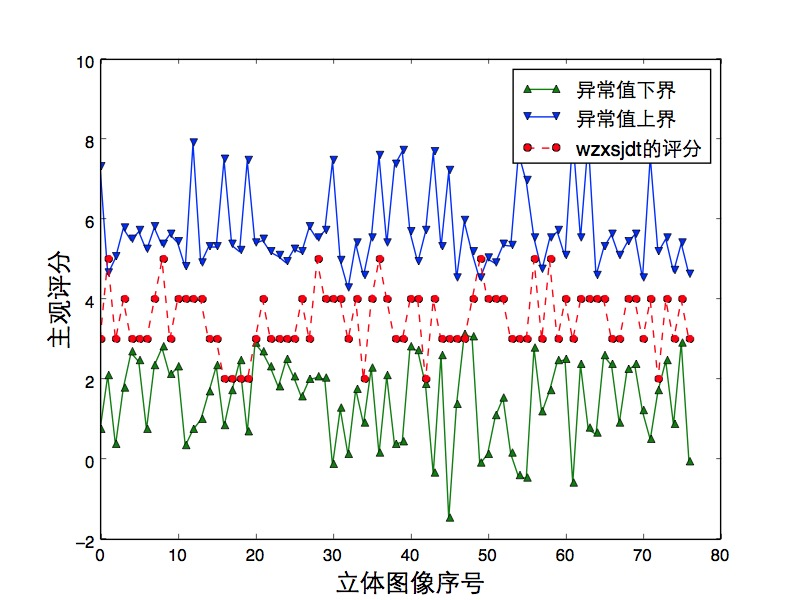
\includegraphics[width=\textwidth]{chap4/exampleofoneperson}
    \bicaption[fig:exampleofoneperson:b]{77幅图像的主观评分的异常评分上界(蓝色)和下界(绿色)以及其中一个被试的评分(红色)}{77幅图像的主观评分的异常评分上界(蓝色)和下界(绿色)以及其中一个被试的评分(红色)}{Fig}{The sup and inf scores for 77 images and the scores from a participant}
  \end{minipage}     
\end{figure}
这个值称为峰度,一般认为当峰度值为3时,数据组服从正太分布。\parencite{recommendation2002500}建议一组数据的峰度值在$[2,4]$之间时,认为该组数据服从正态分布,否则是非正态分布。
我们的主观数据包含77幅图像的评分,每幅图像对应评分的kurtosis系数如图\ref{fig:kurtosis:a}所示。

从图中可以看出,大部分图像的主观评分符合正态分布。

第二,确定合理主观评分的上界${\rm{supS}}$与下界${\rm{infS}}$,\parencite{recommendation2002500}建议的上下界根据评分分布是否服从正态分布可以定义为:
\begin{equation}
{\rm{supS_k = }}\left\{ \begin{array}{l}
{{\bar \mu }_k} + 2*{S_k}{\rm{\qquad              if\  distribution\  is\  normal}}\\
{{\bar \mu }_k} + \sqrt {20} *{S_k}{\rm{\qquad         otherwise}}
\end{array} \right.
\end{equation}
\begin{equation}
{\rm{infS_k = }}\left\{ \begin{array}{l}
{{\bar \mu }_k} - 2*{S_k}{\rm{\qquad              if\  distribution\  is\  normal}}\\
{{\bar \mu }_k} - \sqrt {20} *{S_k}{\rm{\qquad          otherwise}}
\end{array} \right.
\end{equation}
其中${{\bar \mu }_k} $,${S_k}$是所有被试对第$k$幅图像评分的均值与标准差,定义$P_i$,$Q_i$分别表示第$i$个被试的所有评分中超出相应图像评分的上界和下界的次数。即
\begin{equation}
\left\{ \begin{array}{l}
{P_i} = {P_i} + 1{\qquad if\ {u_{ik}} > {\rm{sup}}{{\rm{S}}_k}}\\
{Q_i} = {Q_i} + 1{\qquad if\ {u_{ik}} < {\rm{inf}}{{\rm{S}}_k}}
\end{array} \right.
\end{equation}
其中${u_{ik}}$表示第$i$个被试对第$k$幅图像的评分。
定义局部评分偏大的偏度$Bia{s_{\sup }} $与偏小的偏度$Bia{s_{\inf }}$,$M$表示被试看过的图像总数。
\begin{equation}
Bia{s_{\sup }} = \frac{{{P_i}}}{M} \qquad Bia{s_{\inf }} = \frac{{{Q_i}}}{M}
\end{equation}
根据\parencite{recommendation2002500}的建议,当\textbf{拒绝准则一}:
\begin{equation}
\label{eq:reject1}
Bia{s_{\sup }} > 20\%  \qquad or \qquad Bia{s_{\inf }} > 20\% 
\end{equation}
成立时,则拒绝被试$i$,图\ref{fig:exampleofoneperson:b}给出了其中一个被试的主观评分和图像有效评分的上下界之间的关系。我们实验的结果如图\ref{fig:distributiontestresultforall}所示。
\begin{figure}[!hbp]
  \centering
  \begin{minipage}[b]{0.49\textwidth}
    \captionstyle{\centering}
    \centering
    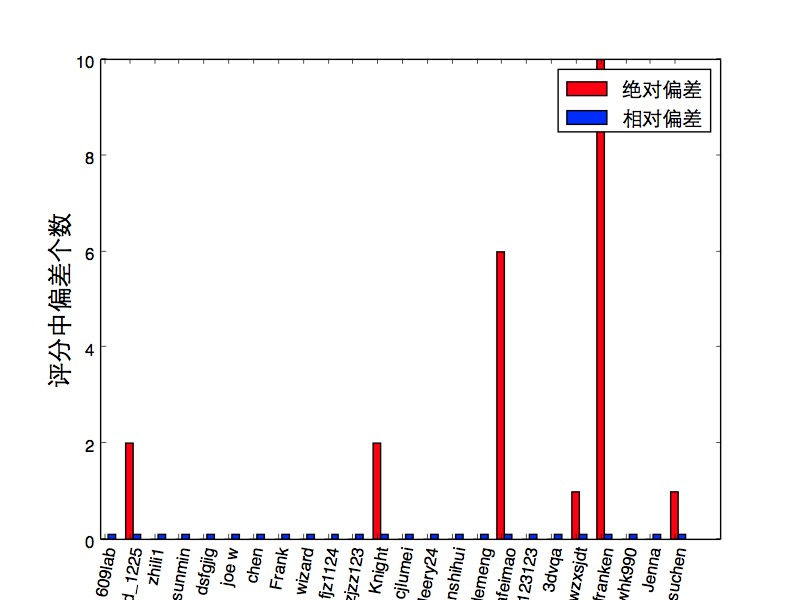
\includegraphics[width=\textwidth]{chap4/outofboundsforallperson}
    \bicaption[fig:distributiontestresultforall]{所有被试评分超出相应图像上界和下界的次数}{所有被试评分超出相应图像上界和下界的次数,这里用0.1代替0}{Fig}{Out of bounds Count for all participant}
  \end{minipage} %  
  \hfill
  \begin{minipage}[b]{0.49\textwidth}
    \captionstyle{\centering}
    \centering
    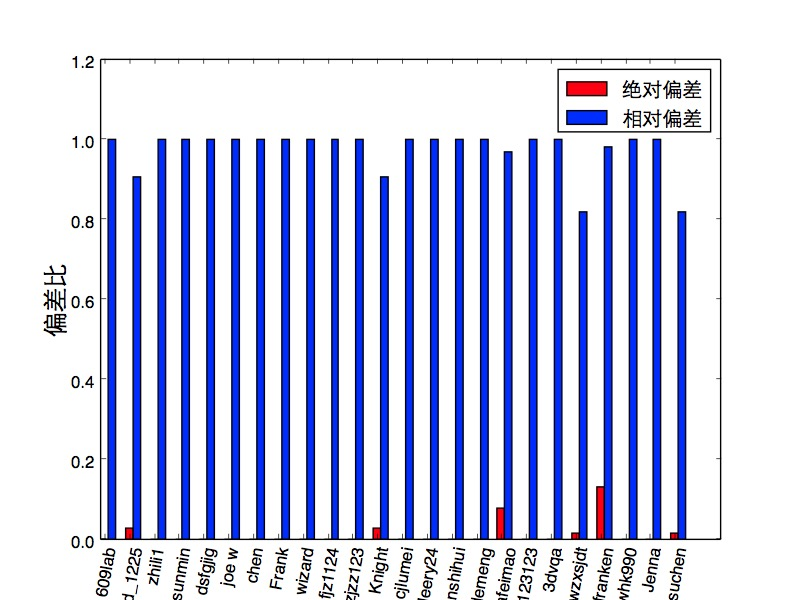
\includegraphics[width=\textwidth]{chap4/absoluteandrelativebiasforall}
    \bicaption[fig:absoluteandrelativebiasforall]{所有被试检验的绝对偏差与相对偏差}{所有被试检验的绝对偏差与相对偏差}{Fig}{The absolute bias and relative bias for all subjects}
  \end{minipage}     
\end{figure}

从图中可以看出,所有被试超出上界次数最多的是“MrFrank”,共计10次,即超出上界偏差最大$Bia{s_{\sup }}=13\%$,没有被试的评分超出下界。根据拒绝准则\ref{eq:reject1},没有用户可以被拒绝。

现在再讨论整体偏差的情况。根据\parencite{recommendation2002500}的建议,定义绝对偏差系数$Bia{s_{abs }}$与相对偏差系数$Bia{s_{relative }}$为:
\begin{equation}
\label{eq:absrelativebias}
\left\{ \begin{array}{l}
Bia{s_{abs}} = \frac{{{P_i} + {Q_i}}}{M}\\
Bia{s_{relative}} = \frac{{\left| {{P_i} - {Q_i}} \right|}}{{{P_i} + {Q_i}}}
\end{array} \right.
\end{equation}
根据\parencite{recommendation2002500}的建议,当\textbf{拒绝准则二}:
\begin{equation}
\label{eq:reject2}
\left\{ \begin{array}{l}
Bia{s_{abs}} > 10\% \\
Bia{s_{relative}} < 30\% 
\end{array} \right.
\end{equation}
成立时,拒绝当前被试$i$。图\ref{fig:absoluteandrelativebiasforall}显示没有被试的相对误差低于30\%,所以,通过上述讨论,没有用户可以被拒绝。
\subsection{图像MOS值估计}
\label{sec:mosevaluation}
通过\ref{sec:dropsinglesubjecterrorvalue}的讨论,我们得到了可以计算MOS值的有效评分。图\ref{fig:mosandconfidence}给出了每幅图像对应的MOS值及其95\%的置信区间。
\begin{figure}[ht]
  \centering
  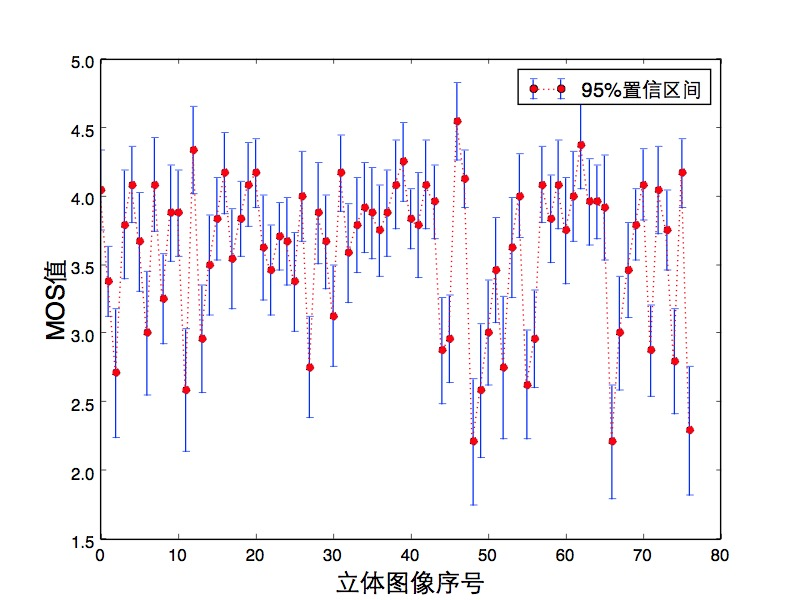
\includegraphics[width=0.6\textwidth]{chap4/mosandconfidence}
  \bicaption[fig:mosandconfidence]{77幅图对应的MOS值及其95\%的置信区间}{77幅图对应的MOS值及其95\%的置信区间}{Fig}{The MOS and 95\% confident interval}
\end{figure}

在\ref{sec:imagedatabase}中创建图像库时本文采用了“移轴法”对选取的11幅图像进行了7种视差调整来获取不同质量的图像。现在将MOS值以相同的移轴值为基准分为7组,然后计算每个被试者对每组图像的MOS值。图\ref{fig:differentdisparity}给出了分组后的评分结果。从图中可以看出:
\begin{figure}[!ht]
  \centering
  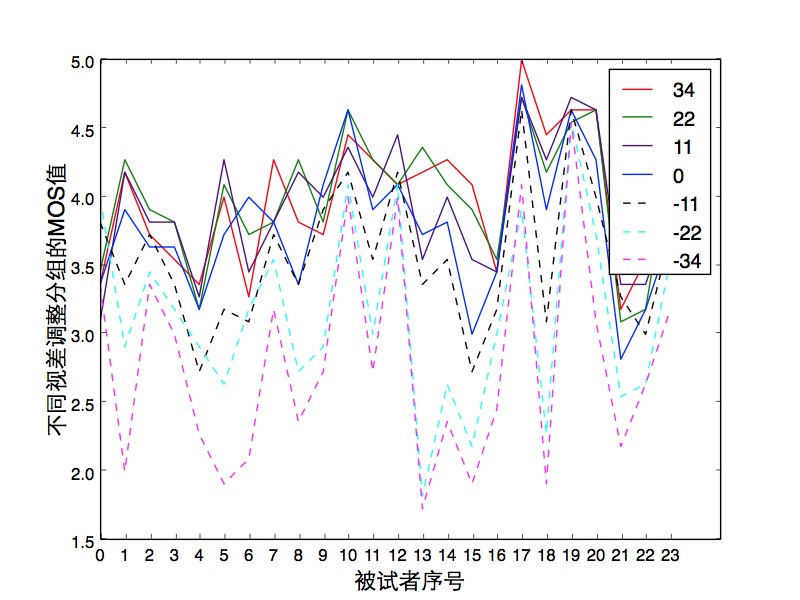
\includegraphics[width=0.6\textwidth]{chap4/differentdisparity}
  \bicaption[fig:differentdisparity]{77幅图按相同的视差调整值分组后24个被试者的MOS值}{77幅图按相同的视差调整值分组后24个被试者的MOS值}{Fig}{The MOS of different shift disparity value}
\end{figure}

第一,图像的主观评分经移轴后确实产生了变化,因此,利用移轴进行视差调整确实可以创建出不同质量的图像。本文的图像库创建方法是合理的。

第二,图像从预设的最舒适的位置开始视差调整,可以看出,视差调整值为正(11,22,34)时,图像质量较好。说明图像内容相对入屏时比较舒适。相反的,当视差调整值为负(-11,-22,-34)时,图像质量偏低。这说明人眼比较习惯观看入屏效果的图像。

第三,图像调整值为正时,图像质量相差不大,这说明人眼在图像相对入屏时容错性更强。而相反的,当调整值为负时,图像质量差异比较明显。图像质量会随着视差调整值的增大而变差。如图中视差调整值为-11和-34的图像质量差别较大。这说明视差调整值为负时人眼对图像质量特别敏感,这与人类在长期的进化过程中眼睛大都看的是相对入屏的场景有关。

本节我们对单刺激主观评分进行处理,主要是对主观评分数据利用ITU-R BT.500-11的标准方法进行了异常值检测。最后结果表明,实验中主观评分的数据不满足局部偏离或整体偏离的条件,均属于可接受的评分。最后,我们获取了与77幅图像对应的MOS值及其95\%的置信区间,并对相同视差调整值下图像的MOS值分布做了分析。MOS值将在第\ref{chap:model}章基于眼动数据建立立体图像质量评价模型时使用。
\section{眼动数据处理}
\label{sec:eyetrackdataprocess}
眼动数据的处理技术我们在\ref{sec:eyetracktechnology}有过综述与介绍,在这部分数据处理中,我们将改进已经成熟的算法,使处理后的数据满足:第一,在精度与准确度方面符合实际需求,第二,适应3D场景的特点。数据的精度与眼动数据的校正过程相关,而数据的准确度则与眼动数据的滤波算法相关。

\subsection{冗余数据剔除}
\label{sec:dropoverdata}
我们的眼动数据来自两部分,第一是3D校正实验,即人眼观看屏幕上产生的随机播放的不同深度不同位置的“目标”时收集的眼动数据;第二是观看立体图像时收集的眼动数据。这两种数据都会产生冗余数据。

首先,对于3D校正实验,由于每个“目标”播放2s钟,当下一个“目标”出现时人眼需要在位置和深度上进行调节,这个过程就会产生一些实际上不在看当前“目标”的视点,如果不剔除这些数据,就会影响最终的校正结果,而校正结果则会影响该被试测量的所有数据,这种系统性的偏差是不可接受的。为了排除这个过程的影响,我们将观看当前目标产生的眼动数据的前0.5s视为冗余数据,在实际处理中将会剔除。

对于观看立体图像时收集的眼动数据,其冗余数据会在两个时刻产生:一是刚开始时,由于我们的眼动数据收集是有任务的收集,即看完图片后还要评分,因此,这个评分的过程会影响到下次观看时人脑的调整速度,所以我们将剔除每幅图像对应眼动数据的第1s的数据。第二,观看结束时会产生冗余,我们的图片播放时长为10s,因为3D图像观看时容易产生视觉疲劳,所以到观看的后期,人的注意力会下降,这时的数据的准确性会降低。因此,我们将最后1s的数据视为冗余数据,处理时剔除。
\subsection{基于视差角的眼动数据3D校正}
\label{sec:calibraiton}
在\ref{sec:eyetrackcalibration}我们提到,眼动仪会自带一个原生的2D校正算法,实验中采用的Tobii眼动仪无论是提供给我们的studio软件还是Tobii SDK开发包,都包含了这部分功能。因此,本文对眼动仪的2D校正算法不再做讨论,而是对其3D校正过程做一下详细描述。

眼动数据的3D校正过程依赖于第三章的3D校正实验,在第三章的实验中,我们采用了25点法来替代Wang的算法\parencite{wang2014online}中的Lissajous-knot path,这25个点分别分布在5个深度平面上,每个平面上5个点的位置分别为(0.1,0.1), (0.1,0.9), (0.5,0.5), (0.9,0.1), (0.9,0.9),这里我们用(0,0)表示屏幕的左上角,而(1,1)表示屏幕的右下角。其对应的视差以像素记为-30, -10, 0, 10, 30 ,相应地视差角可以表示为$ -{0.5345^\circ }, -{0.1782^\circ }, {0^\circ }, {0.1782^\circ }, {0.5346^\circ }$,每个点在屏幕上随机播放2s。眼动仪的采样频率为60Hz,即每个目标对应120个采样点。由于采样初期人眼捕捉目标需要时间,因此,针对每个目标的数据,去掉前0.5s的采样点集,防止引入较大误差。

对于3D校正算法,在我们前面的工作中\parencite{ma2015new},采用了Wang\parencite{wang2014online}的算法,该算法可以描述为:依据预设的视差值,利用拉格朗日最小均方差\parencite{lancaster1986curve}对称的对测量视差值做平移与尺度变换,这里称该算法为基于视差偏差的3D校正算法。对于每个采样点 $j$, ${D_j}$表示当前观看目标预设的视差值,而 ${D'_j}$表示眼睛实际测量到得视差值,该值可以通过双目注视点横坐标之差来估计:
\begin{equation}
\label{eq:disparitypixel}
{D'_j} = {G'_{Rx}} - {G'_{Lx}},
\end{equation}
这里$G'_{Rx}$ 表示右眼注视点在屏幕上的横坐标,而 $G'_{Lx}$ 表示左眼注视点的屏幕上的横坐标。 用一个一阶模型来最小化测量值与预设值之间的误差,假设${a_0}, {a_1}$表示一阶模型的未知项,则该模型可以表示为:
\begin{equation}
[{d_j}] = [1\;\;{d'_j}]{\left[ {{a_0}\;\;{a_1}} \right]^T}.
\end{equation}
其中${d_j},{d'_j}$分别表示测试时刻$j$的预设视差与测量视差。这样,就可以构造一个线性系统:
\begin{equation}
\textbf{D} = \textbf{D}'\textbf{a}
\end{equation}
这里$\textbf{D}$表示已知的视差值(pixel) ,$\textbf{D}'$ 是根据眼动数据计算的视差值(pixel)。由于已知条件个数超过了未知数的个数,所以该线性系统在这里是过约束的,其解为:
\begin{equation}
\textbf{a} = {({\textbf{D}'^T}\textbf{D}')^{-1}}{\textbf{D}'^T}\textbf{D}
\end{equation}
至此,视差的校正结果可以描述为:
\begin{equation}
\label{eq:3dcalibration}
{D_j} = {a_0} + {a_1}*{D'_j}.
\end{equation}
现在将校正过的视差值反馈到左右注视点,根据方程\ref{eq:3dcalibration}可以得到眼动数据测量值的偏差:
\begin{equation}
\label{eq:errorcal}
{\varepsilon_j} = {D_j} - {D'_j}
\end{equation}
将偏差均匀的补偿给左右眼,其结果为
\begin{equation}
\label{eq:servertoeye}
\left\{ \begin{array}{l}
{G_{Lx}} = {{G'}_{Lx}} - \varepsilon_j /2,\\
{G_{Rx}} = {{G'}_{Rx}} + \varepsilon_j /2.
\end{array} \right.
\end{equation}

现在来改进该算法,以适应眼动数据测试条件。先来分析我们的测试条件与Wang的测试条件的不同,两种实验条件见图\ref{fig:conditioncompare}。
\begin{figure}
  \centering
  \subfigure[我们的测试场景]{
    \label{fig:ourcondition:a} %% label for first subfigure
    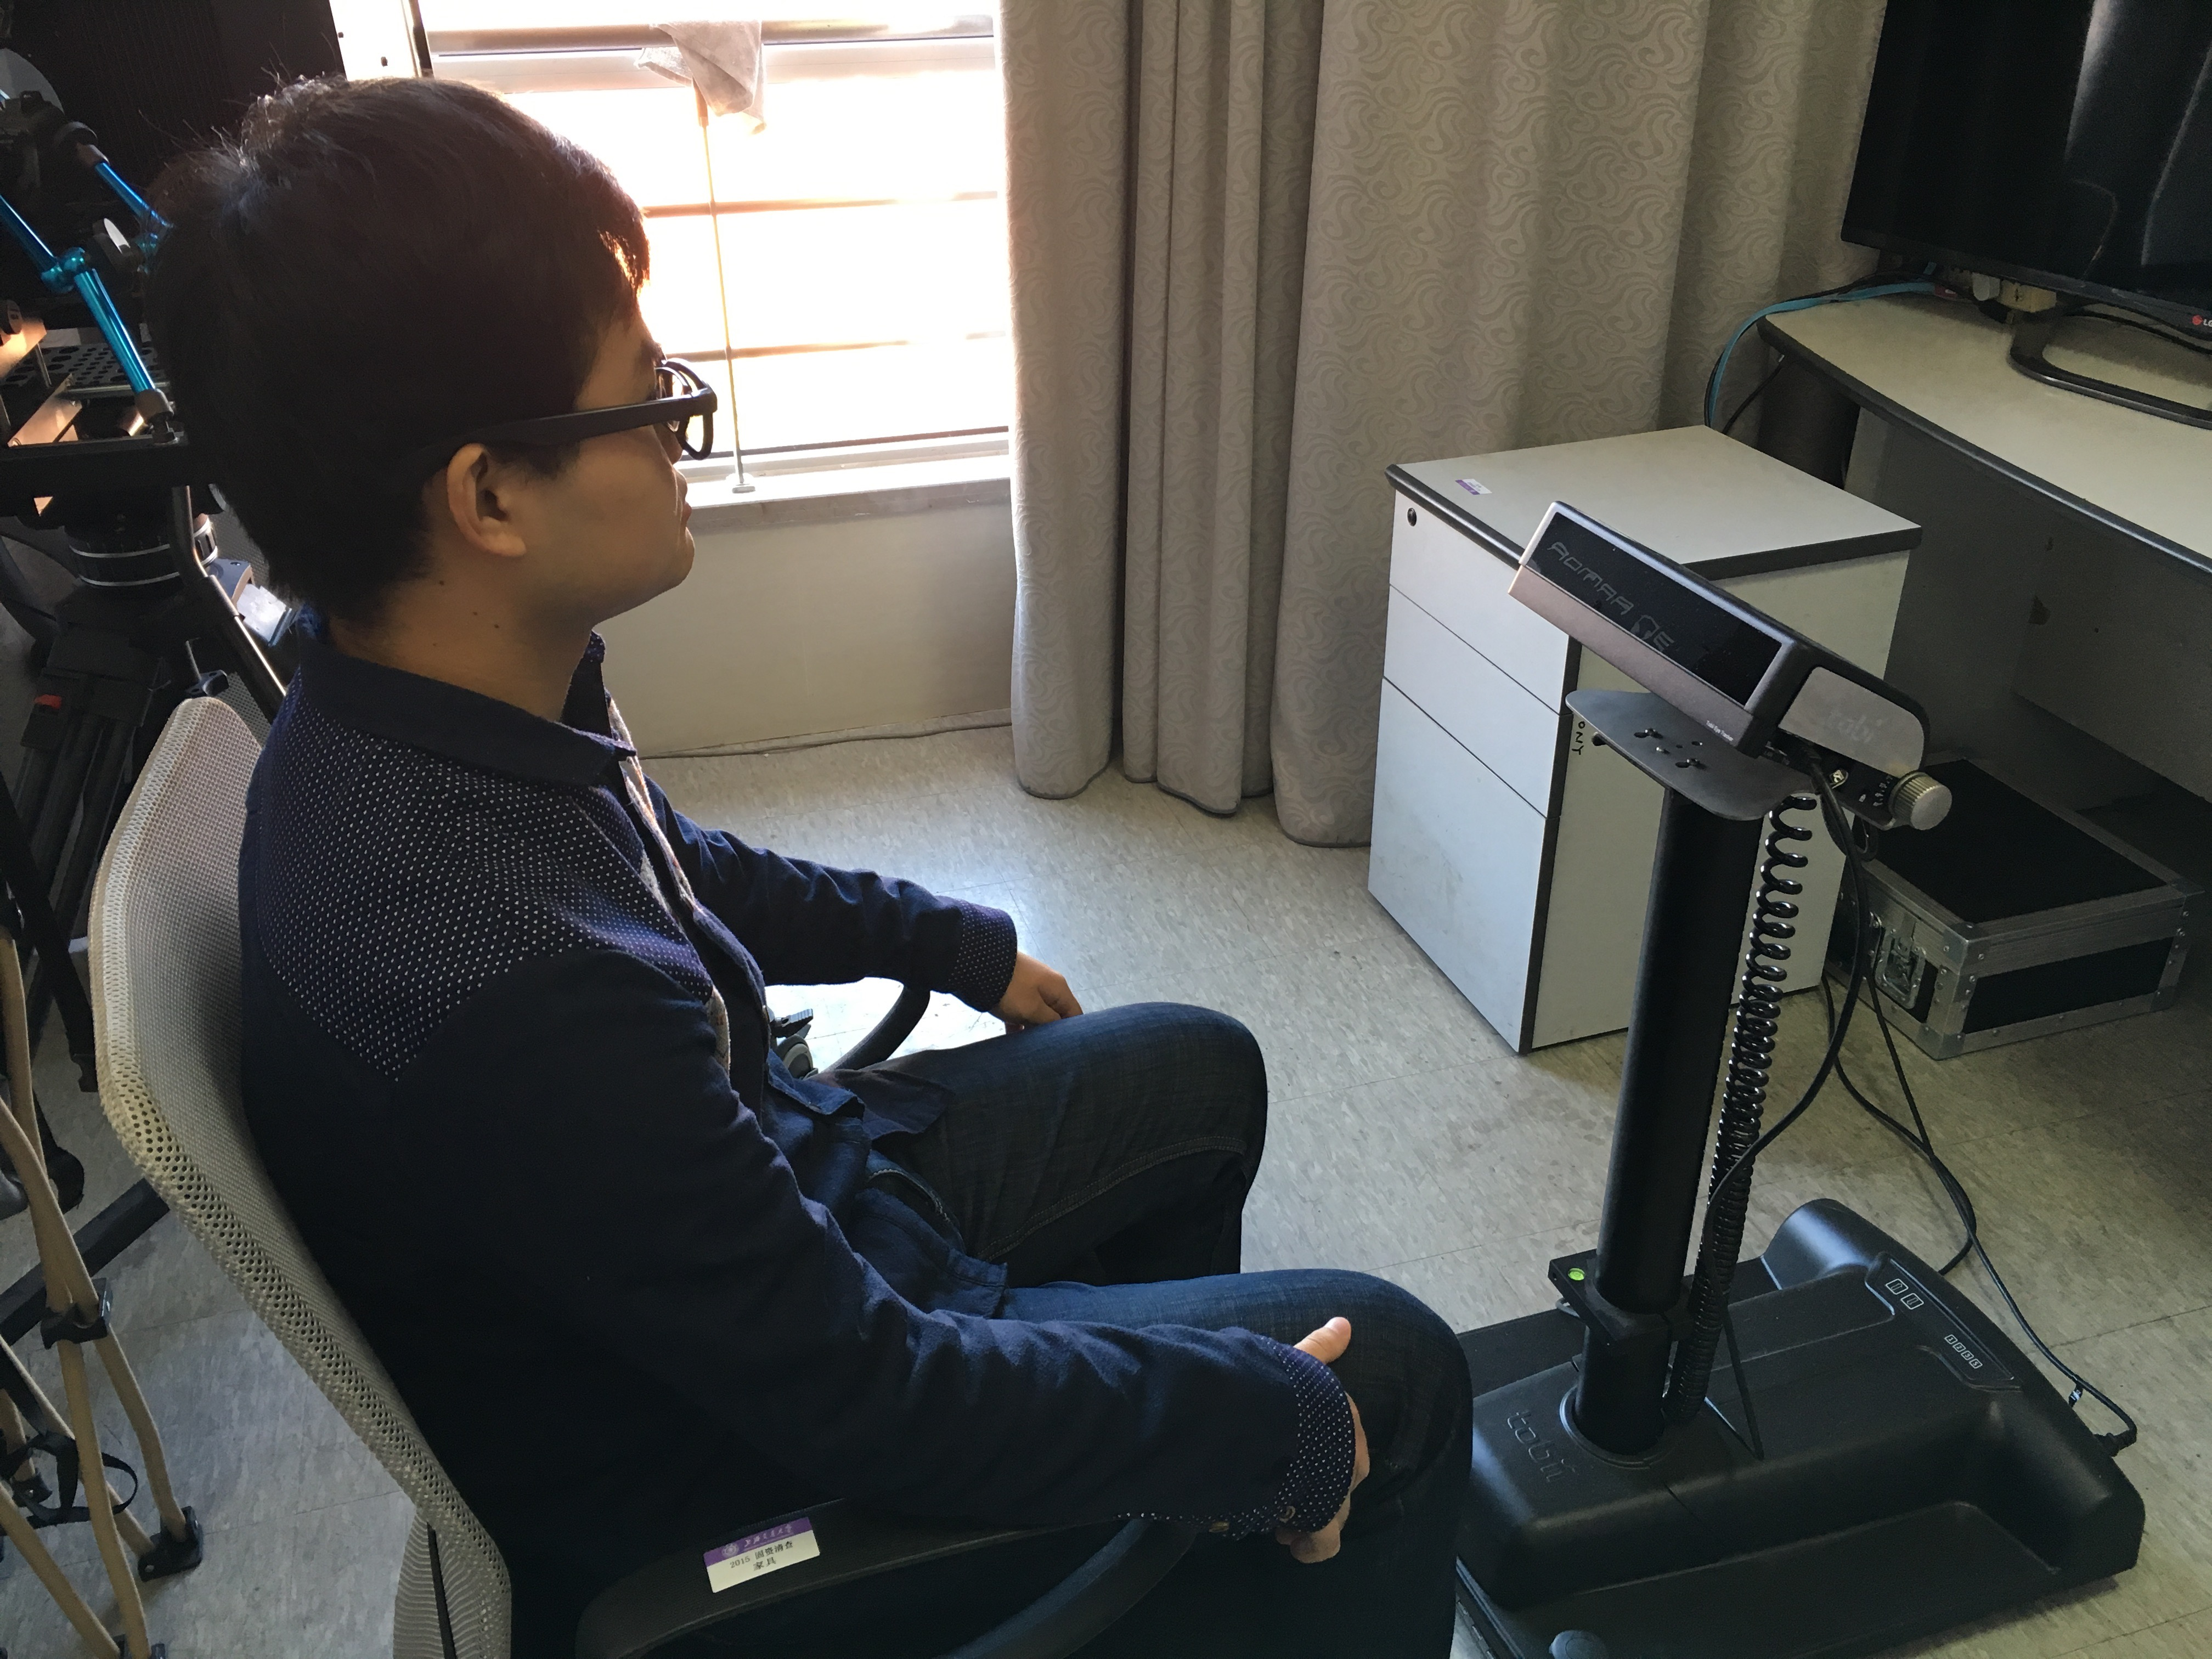
\includegraphics[width=0.3\textwidth]{chap4/ma.jpg}}
  \hspace{1in}
  \subfigure[Wang的测试场景]{
    \label{fig:wangcondition:b} %% label for second subfigure
    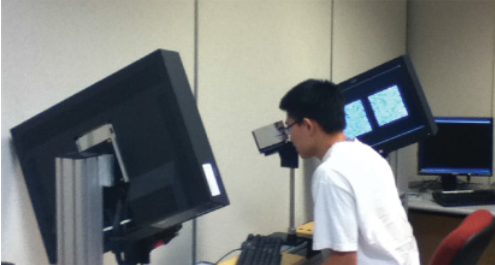
\includegraphics[width=0.4\textwidth]{chap4/wang.png}}
  \bicaption[fig:conditioncompare]{两种数据采集场景对比}{两种数据采集场景对比}{Fig}{The difference between Wang's and our condition}
\end{figure}
\begin{figure}[t]
  \centering
  \subfigure[校正前的测量数据]{
    \label{fig:beforecalibration:a} %% label for first subfigure
    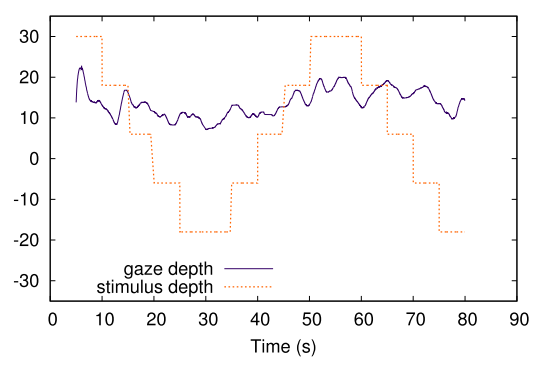
\includegraphics[width=0.45\textwidth]{chap4/beforecalibration.png}}
  \subfigure[校正后的数据]{
    \label{fig:aftercalibration:b} %% label for second subfigure
    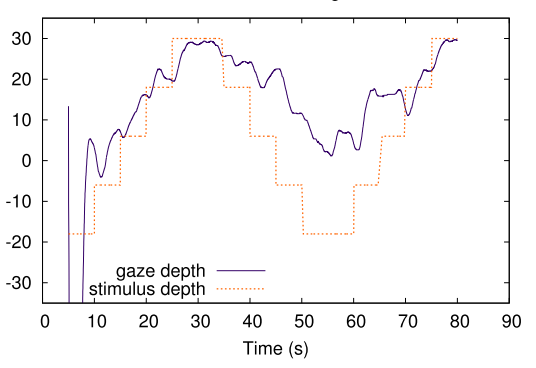
\includegraphics[width=0.45\textwidth]{chap4/aftercalibration.png}}
  \bicaption[fig:performanceofcalibration]{校正前后的效果对比图}{校正前后的效果对比图}{Fig}{The difference between before and after calibration}
\end{figure}
由图\ref{fig:conditioncompare}可见,Wang的眼动仪与头部的位置相对固定,是准侵入式设备。而我们的眼动仪则是非侵入式装备,两者的最大区别在于头部是否可动。在\ref{sec:caldisparity}中本文曾经分析了与视差角相关的量:眼睛的位置和屏幕上的注视点的位置。可见在Wang的测试条件下,由于眼睛位置相对来说比较固定,所以视差实际上由屏幕上的注视点来确定,这就是Wang的算法直接采用方程\ref{eq:disparitypixel}计算视差的原因。而我们的实验条件决定了人的头部是可动的,这就使得眼睛的位置相对不太固定,如此,直接采用方程\ref{eq:disparitypixel}计算视差的精度较低。所以,本文的算法对视差信息的估计采用视差角来表示,见方程\ref{eq:disparityofeyetrackdata}。

我们的改进方法称为基于视差角偏差的3D校正算法:
第一,利用方程\ref{eq:disparityofeyetrackdata}求得预设的视差角$\theta_j$和实际测量的视差角$\theta'_j$,仍然用一个线性系统来进行平移与尺度变换。设未知参数为$\textbf{a} = \left[ \begin{array}{l}
a\\
b
\end{array} \right]$,则此时线性系统可以表述为
\begin{equation}
\Phi  = \Phi '\textbf{a}
\end{equation}
这样我们就可以利用已知量得到该系统的解为:
\begin{equation}
\textbf{a} = {({\Phi'^T}\Phi')^{-1}}{\Phi'^T}\Phi
\end{equation}
其中$\Phi'=[\theta'_j],\Phi=[\theta_j]$.此时,视差角的校正过程如下:
\begin{equation}
\label{eq:3dcalibrationangular}
{\theta_j} = {a_0} + {a_1}*{\theta'_j}.
\end{equation}
至此,我们得到了校正后的视差角,如何将测量的偏差补偿呢?我们利用校正后的视差角计算出其在屏幕上对应的视差值(pixel)
\begin{equation}
\label{disparityfromangulartopixel}
D(pixel) = \left[ {e - 2d*\tan (\arctan (\frac{e}{{2d}}) - \frac{\theta }{2})} \right]*\frac{{{R_x}}}{W}
\end{equation}
其中$D$是像素单位的视差,$e$是人眼双目距,可以根据双目坐标求得,$d$为人眼到屏幕的距离,$\theta$是视差角。$R_x$表示屏幕的水平像素,$W$表示屏幕的宽。
此时的偏差仍然用方程\ref{eq:errorcal}来估计,最后的校正用方程\ref{eq:servertoeye}来完成,图\ref{fig:performanceofcalibration}给出了其中一个测试者校正前后的效果。
\begin{figure}[t]
  \centering
  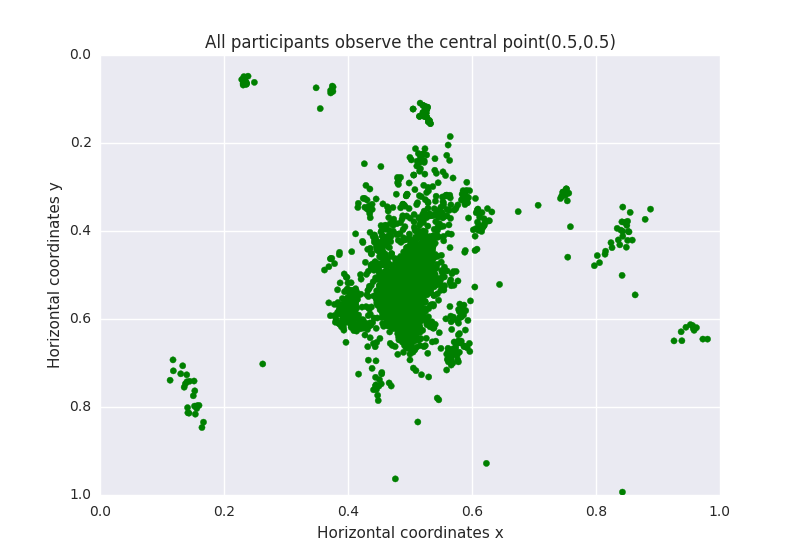
\includegraphics[width=0.5\textwidth]{chap4/rawdatadistribution}
  \bicaption[fig:rawdatadistribution]{所有实验被试观看屏幕中心点时眼睛注视点的散点图,这里我们设定屏幕左上角为(0,0),右下角为(1,1)}{所有实验被试观看屏幕中心点时眼睛注视点的散点图,这里我们设定屏幕左上角为(0,0),右下角为(1,1)}{Fig}{The scatter map of all gazepoints from participant,where(0,0)denotes upper left corner while (1,1) denotes right bottom}
\end{figure}
\subsection{基于辅眼的眼动数据滤波}
\label{sec:filter}
前面已经提到了眼动过程包含三种可能的过程,即注视过程、扫视过程以及眨眼等无法被眼动仪捕捉到得过程。眼动数据滤波的主要目的是除去噪声以及从眼动数据中分离出这些过程。众所周知,当眼睛注视一个区域时,眼睛事实上一直在颤抖,这个过程称为眼颤。眼颤的结果是当人眼注视某一点时,实际上注视了环绕该点的一片区域,而眼动仪确实会记录到这些数据,如图\ref{fig:rawdatadistribution}是所有的实验参与者观看在屏幕中心的点(0.5,0.5)的散点图。从图中可以看出,注视区域的中心与我们设定的点基本重合,但是显然,除了一些记录错误的点,其它的点都是围绕在中心注视点附近的。而这些数据就引入了噪声。因此,在眼动数据滤波这一部分,本文要解决两个问题,一个是如何确认眼动数据中的噪声以及去噪,另一个是如何从眼动数据中分离出注视过程和扫视过程。

先来分析噪声数据的类型,由于点的坐标由横纵坐标组成,我们来分析注视一个点得时候视点的横纵坐标的分布。
图\ref{fig:gazepointdistribution}给出了所有视点的横纵坐标的分布图。图\ref{fig:histmap:a}和\ref{fig:densitymap:b}清楚的表明,注视一个点时,视点的横纵坐标均符合高斯分布。即眼动数据包含的噪声表现为高斯白噪声。
因此我们在滤波时主要任务是除去数据中的高斯白噪声。
\begin{figure}[ht]
  \centering
  \subfigure[所有视点的横坐标和纵坐标分布直方图]{
    \label{fig:histmap:a} %% label for first subfigure
    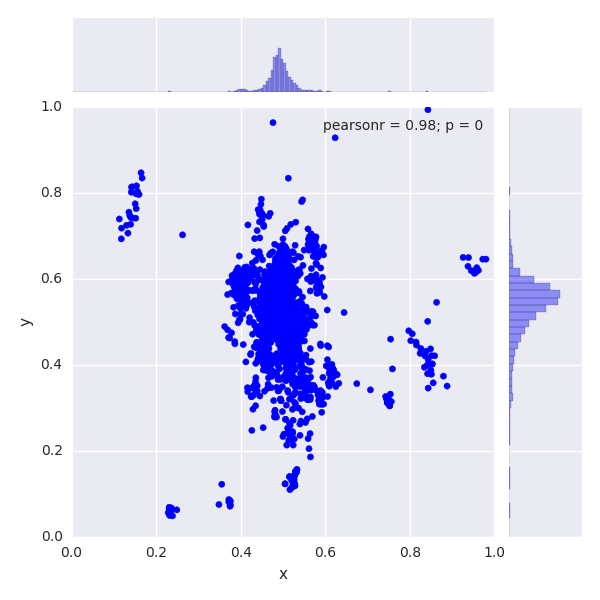
\includegraphics[width=0.47\textwidth]{chap4/eyemovehistmap}}
  \subfigure[所有视点的横坐标和纵坐标分布密度图]{
    \label{fig:densitymap:b} %% label for second subfigure
    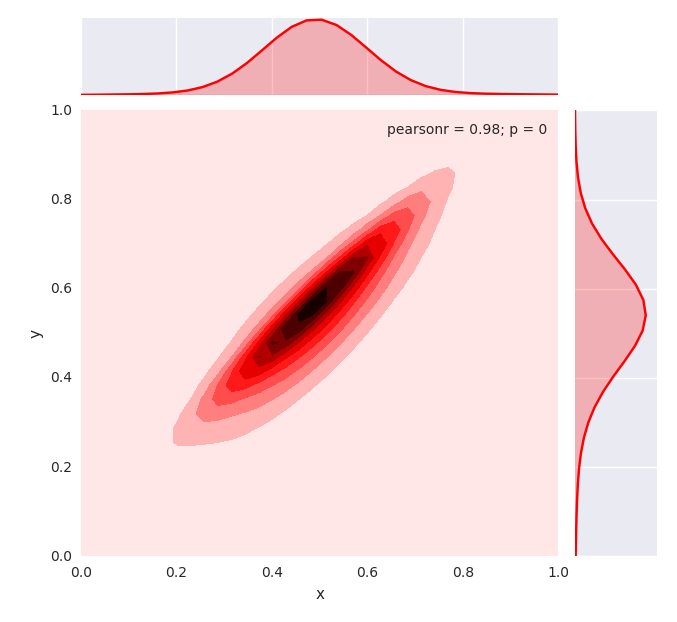
\includegraphics[width=0.47\textwidth]{chap4/eyemovedensitymap}}
  \bicaption[fig:gazepointdistribution]{所有视点的横纵坐标分布图}{所有视点的横纵坐标分布图}{Fig}{The x,y distribution of gazepoints}
\end{figure}
\parencite{duchowski2007eye}中提到,眼动过程中扫视点持续的时间大约是$30ms \sim 120ms$,注视点持续的时间是$150ms \sim 600ms$,两个扫视过程之间就是一个注视点。因此,要想分离扫视过程与注视过程,如果可以判定扫视过程,那么自然就可以判定注视过程。
扫视过程有两个特点:第一,持续时间短;第二,注视过程中会出现大的跳跃。结合这两个特征,本文仍然采用\parencite{olsson2007real}中累积距离差之和最大的方法来解决问题。我们给出这个算法的概要:

第一,根据扫视过程的持续时间,定义一个窗$L$,由于其最长持续时间是$30ms \sim 120ms$,眼动仪的采样率为60Hz,每个采样点约占16.7ms,所以一个扫视过程最少占两个采样点,最多占7个采样点,为了找出大多数的扫视点,我们取窗长为5个采样点;

第二,计算时间上相邻两个视点的距离,形成一个距离序列$D$;

第三,用长度为5的窗$L$从距离序列$D$的前五项开始,计算窗内和,让窗逐步移向$D$的尾部移动直到窗体右端到达$D$的结尾,形成窗内累积和序列$S$;

第四,当S中存在的项$s_i$满足$s_i>s_{i-1}$且$s_i>s_{i+1}$时,则此时$s_i$对应的窗内的序列就是扫视序列,相邻的区域则为注视序列。

第五,由注视序列估计注视点。由于眼动数据中的噪声为高斯白噪声,因此,取注视序列中的中值来估计该注视点,这相当于采用了中值滤波的方法来消除高斯噪声。
\begin{figure}[!htp]
  \centering
  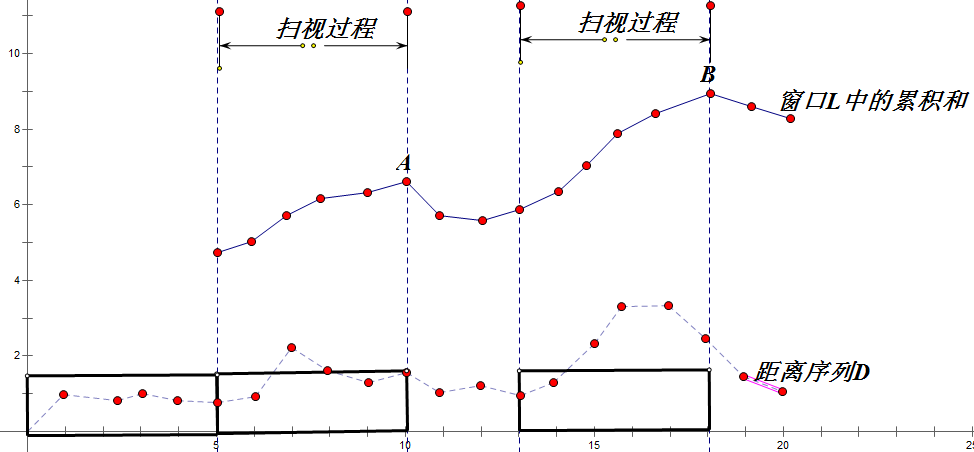
\includegraphics[width=0.6\textwidth]{chap4/windowL}
  \bicaption[fig:windowL]{基于固定窗的扫视点检验方法示意图}{基于固定窗的扫视点检验方法示意图,图中虚线是相邻两视点的欧式距离,实线为固定窗口L中的距离和。$A,B$两点满足比前后位置值都大,所以,此刻窗口对应的序列为扫视序列}{Fig}{The saccade point detecting of eyetracking data based on window L,The windows are saccade points corresponding to $A,B$}
\end{figure}
\begin{figure}[t]
  \centering
  \subfigure[滤波结果示意图1(主眼)]{
    \label{fig:filterresults:a} %% label for first subfigure
    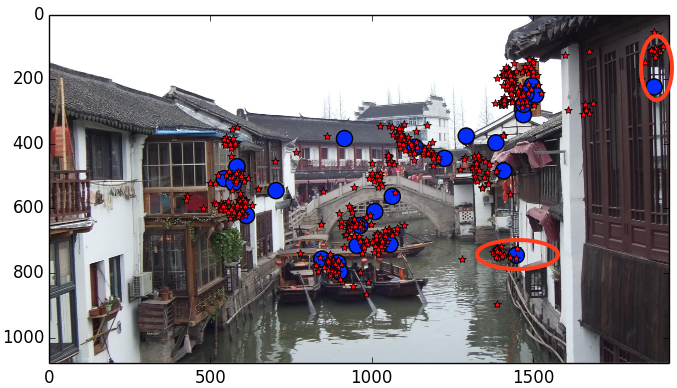
\includegraphics[width=0.45\textwidth]{chap4/filterresults2_R}}
  \subfigure[滤波结果示意图1(辅眼)]{
    \label{fig:filterresults:b} %% label for second subfigure
    \includegraphics[width=0.45\textwidth]{chap4/filterresults2_L}}
      \subfigure[滤波结果示意图2(主眼)]{
    \label{fig:filterresults:c} %% label for first subfigure
    \includegraphics[width=0.45\textwidth]{chap4/filterresults3_R}}
  \subfigure[滤波结果示意图2(辅眼)]{
    \label{fig:filterresults:d} %% label for second subfigure
    \includegraphics[width=0.45\textwidth]{chap4/filterresults3_L}}
  \subfigure[滤波结果示意图3(主眼)]{
    \label{fig:filterresults:e} %% label for first subfigure
    \includegraphics[width=0.45\textwidth]{chap4/filterresults4_R}}
  \subfigure[滤波结果示意图3(辅眼)]{
    \label{fig:filterresults:f} %% label for second subfigure
    \includegraphics[width=0.45\textwidth]{chap4/filterresults4_L}}
  \bicaption[fig:filterresults]{同一幅图对应的眼动数据在不同参考眼睛下进行滤波与眼动过程分离后的结果}{同一幅图对应的眼动数据在不同参考眼睛下进行滤波与眼动过程分离后的结果,图a,c,e是以主眼为参考滤波的结果,图b,c,f是相应的以辅眼为参考滤波的结果。}{Fig}{The result of filtered and eyemovement seperate.}
\end{figure}

第六,以辅眼视点为参考进行滤波。在算法步骤二需要计算时间上相邻的两个视点间的距离,选用哪个眼睛作为参考眼睛是一个问题。一般在2D模式下,考虑的是人眼在屏幕上的注视点,所以,通常采用两眼注视点的平均位置作为参考。但是在3D模式下,双眼看到的图片不同,且双眼在立体视觉中的功能不同——主眼负责控制方向,辅眼辅助形成深度视觉。所以,考虑两个眼睛注视点的平均位置不太适用。到底选用主眼还是辅眼作为参考,我们对两种情形都进行了对比实验,图\ref{fig:filterresults}给出了同一幅在两种参考眼睛下滤波的结果。其中左边为以主眼为参考滤波的结果示意图,右边是以辅眼为参考滤波结果示意图。图中“*”表示未处理视点(Gaze point)位置,圆圈表示估计的注视点(Fixation point)位置,这里以图\ref{fig:filterresults:a}和图\ref{fig:filterresults:b}的结果为例来做分析:

首先,从图中可以看出,本文估计的注视点大部分都位于原始视点密集的地方,如图\ref{fig:filterresults:b}中矩形标注的区域。也有少部分注视点为错误的估计,如图\ref{fig:filterresults:b}中六边形标记的区域,这可能是注视时间过短的点造成的遗留,未来的算法的改进中应该考虑去除长度太短的点。另外,有些密度大的区域的注视点过于密集,这主要与观看的时间前后有关,即某一区域在$t_1$时刻被注视,过了一段时间到$t_2$时刻又被注视,此时的注视点虽然在同一个区域,但是是不同的注视点。这也是传统的聚类算法在分离眼动过程中不可用的原因。总体来看,本文的眼动过程分离算法是有效的。

其次,来分析主眼与辅眼分别为参考的滤波结果,图\ref{fig:filterresults:a}和图\ref{fig:filterresults:b}清晰的表明,以辅眼为参考眼估计的注视点精度更高,如图中椭圆标记的区域。以上结论同时可以在图\ref{fig:filterresults:c}和图\ref{fig:filterresults:d}以及图\ref{fig:filterresults:e}和图\ref{fig:filterresults:f}中看出。

最后,在第\ref{chap:model}章中进行特征提取时,发现以辅眼为参考滤波的数据提取的特征性能更优,这也从另一方面证明了采用辅眼为参考滤波的正确性。
\subsection{立体场景下眼动数据的可视化表示}
\label{sec:densitymap}
采集好的眼动数据一般以数据库或文本的形式存储,这种表示方法对于直观分析眼动结果没有任何作用。而可视化的表示方法则可以清楚地描述眼睛注视的区域,注视过程等。立体图像的眼动数据如何可视化表示呢,这是本小节要解决的问题。

一种可选的方法是直接选择传统的2D眼动数据注视密度图——灰度图与伪彩色图。图\ref{fig:2ddensitymap:b}和\ref{fig:2ddensitymapgray:c}分别是所有的被试观看实验图片\ref{fig:origimage:a}的眼动数据注视密度图,从图上可以很清楚的获取人眼注视的区域等信息。

但是,正如在\ref{eyetrackdatarepresentation}讨论的一样,3D场景下,除了2D信息之外,还包括了立体视觉最重要的信息之一——深度信息。但是上述两种方法都不能有效的表示出深度信息。因此,本节将提出一种为立体图像创建注视密度图的表示方法——3D图像注视密度图(Fixation density map)。此方法首先提出一种新的3D图像的表示方法,然后在此基础上将眼动数据依据图像分层深度也进行分层,并创建相应层的2D注视密度图,最后将各层分布在对应的深度层上形成立体表示。
\begin{figure}[!t]
  \centering
    \subfigure[伪彩色图示意图]{
    \label{fig:2ddensitymap:b} %% label for first subfigure
    \includegraphics[width=0.4\textwidth]{chap4/2ddensitymap}}
  \subfigure[灰度图示意图]{
    \label{fig:2ddensitymapgray:c} %% label for second subfigure
    \includegraphics[width=0.4\textwidth]{chap4/2ddensitymapgray}}
    \subfigure[示意图73s34.jpg]{
    \label{fig:origimage:a} %% label for first subfigure
    \includegraphics[width=0.5\textwidth]{chap4/73s34}}
  \bicaption[fig:densityexample]{2D眼动数据图常见的表示方法}{2D眼动数据图常见的表示方法}{Fig}{The density map for 2D image}
\end{figure}
\subsubsection{基于视差图分割的立体图像分层分割的立体表示方法}
\label{sec:stereoscopicimagerepresentation}
我们的目的是创建一种注视密度图,该图不仅可以反映用户看了什么地方,还可以反映出看的地方的深度。因此,需要一种图像的立体表示方法。而当前主流的 3D 图像的格式,如左右分离,左右合成,上下合成,交错格式,互补色格式,2D+depth等,从 本质上来说就是 2D 图像,其立体效果需要3D设备(如支持各种格式的显示器和偏振光片)的辅助才能感知到。所以,这些传统的方法无法满足当前的需求。因此,本文将在深度方向进行分割,依据视差图的信息,将图片近似的分割成若干个层次,这样,就可以近似的知道图像中各部分的深度信息。这种做法需要解决两个问题:第一,视差图的提取要较为准确。这是我们分割图像的基础,视差图提取越准确,则分割的越精确。当前提取3D图像深度的方法日趋成熟。Scharstein\parencite{scharstein2002taxonomy} 、Gangwal\parencite{gangwal2009depth}等都给出了精度很好地深度提取算法。Zhou\parencite{zhou2015depth}的工作的算法效果也很好,这里我们采用该算法。第二,图片在深度方法进行分割,最小的分割区间如何确定。与立体视觉相关的一个重要的视觉特征是人眼的立体视敏度,即人眼分辨在深度方向上相邻物体空间位置关系的能力。研究发现,在好的光线条件下,人眼的立体视敏度 可以达到 $2\sim6{\mathop{\rm arc\ sec}\nolimits} $(弧秒),而在一般情况下,人眼的立体视敏度可以为 2.3 arc min(弧分)\parencite{coutant1993population},这就为在深度方向上分割图像时确定分割步长提供了依据。

基于上述分析,这里先给出该方法的总体方案,该方案包括五个模块:
\begin{itemize}[noitemsep,topsep=0pt,parsep=0pt,partopsep=0pt]
\item 立体图像视差图提取模块,用于得到与该立体图像中参考图像相对应的视差图 $D$;
\item 立体图像深度区间设置模块,用于根据立体图像的视差特征及用于显示立体图
像的3D显示器及人眼观看的环境参数,设置该立体图像的整体深度区间; 
\item 立体图像深度平面设置模块,用于根据立体图像的视差分布特征及 3D 显示器
的环境参数,根据人眼立体视敏度设置合适的深度平面数及各深度平面间的深度区 间步长;
\item 深度层图像分割模板生成模块,用于依据所设置的深度平面数及深度区间步长,
利用视差图所反映的深度特征,分割得到各深度层对应的图像分割模板;
\item 参考图像区域分割及深度分层显示模块,用于利用所得到的各深度层对应的图
像分割模板对原图像进行分割,得到各深度平面上的图像内容,并将各深度平面上 的图像内容显示在一个立体空间中。
\end{itemize}
具体流程图如图\ref{fig:newrepresentationprocedure}所示
\begin{figure}[ht]
  \centering
  \includegraphics[width=0.3\textwidth]{chap4/newrepresentationprocedure}
  \bicaption[fig:newrepresentationprocedure]{立体图像分层表示流程图}{立体图像分层表示流程图}{Fig}{The procedure of new approach}
\end{figure}
这里我们以图\ref{fig:52L:a}为例来说明整个方法的操作过程。
\begin{figure}
  \centering
  \subfigure[示例立体图像左图]{
    \label{fig:52L:a} %% label for first subfigure
    \includegraphics[width=0.4\textwidth]{chap4/52L}}
  \hspace{1in}
  \subfigure[与示例图像对应的视差图]{
    \label{fig:52_L_depthMap:b} %% label for second subfigure
    \includegraphics[width=0.4\textwidth]{chap4/52_L_depthMap}}
  \bicaption[fig:exmpleImage]{示例立体图像的左图和视差图}{示例立体图像的左图和视差图}{Fig}{The original left image and disparity map}
\end{figure}
%%%%%%%%
\\[0.2cm]
\noindent{\textbf{\emph{a.立体图像的视差提取}}}
\\[0.2cm]
\indent{本文}使用Zhou\parencite{zhou2015depth}的算法来提取视差,其效果图如图\ref{fig:52_L_depthMap:b}所示,可以看出,该算法能很好地获取立体图像的视差图。当视差信息被表征为深度图,需要按照视差图到深度图的逆映射反变换出视差图。同时,在这里得到了图像的最大视差值$D_{max}$和最小视差值$D_{min}$。
%%%%%%
\\[0.2cm]
\noindent{\textbf{\emph{b.设定深度区间}}}
\\[0.2cm]
\indent{深度}区间的设置与3D观看环境和立体图像的视差范围有关,给定3D电视及其屏幕参数,假设 $W$, $H$ 分别表示屏幕的高和宽(cm)。屏幕的分辨率可以表示为${R_x}\times{R_y}$像素。根据 ITU-R BT500-12\parencite{itu500,},人眼到屏幕的最佳距离$d$ 为3倍屏高:$d = 3*H$。另一个重要参数是人眼双目距$e$(一般认为,$e$的均值为6.5cm)。假设人眼关于屏幕中心垂线对称,就可以根据\ref{sec:stereodisparity}立体场景下视差的定义计算视差角。根据图\ref{fig:disparitydifinition},便可以获取人眼在屏幕上的汇聚角 $\alpha$:
\begin{equation}
{\alpha  = 2\arctan (\frac{e}{{2d}})}
\end{equation}
同理,可以得到双目在空间中的汇聚角$\gamma$ 或$\beta$。视差角定义为双目在屏幕上的汇聚角与在空间中的汇聚角之差。此时与视差值$D$(pixel)对应的视差角 $\theta$ 的表达式为:
\begin{equation}
\label{eq:chap4:disparitycal}
\begin{array}{l}
\theta  = 2*(\arctan (\frac{e}{{2d}}) - \arctan (\frac{{e - {D_m}}}{{2d}}))\\
{D_m} = \frac{{D*W}}{{{R_x}}}
\end{array}
\end{equation}
从\ref{eq:chap4:disparitycal}可以看出,当左右图的对应点在屏幕上的视差值  $D=0$时,视差角$\theta=0$,也就是双目汇聚在了屏幕上。
通过 \textbf{\emph{a}}部分已经得到了图像的最大最小视差值${D_{\max}}$  and ${D_{\min}}$,根据方程\ref{eq:chap4:disparitycal},就可以计算出相应的最大最小视差角$\theta _{\max }^I$和$\theta _{\min }^I$。

在这里还将考虑另一个问题,立体图像的舒适度,由于视差是影响立体图像舒适度最大的因素之一,因此,本方法将标注出舒适范围和不舒适范围。一般认为,当视差处于$( - 1^\circ , + 1^\circ )$时,图像的舒适度比较好\parencite{lambooij2009visual},超出这个范围的部分其舒适度较低。而舒适区域的部分将是我们考虑的重点。所以将分割的深度范围设定为:
\begin{equation}
(\theta _{\min }^R,\theta _{\max }^R) = (\max ( - {1^\circ },\theta _{\min }^I),\min ( + {1^\circ },\theta _{\max }^I))
\end{equation}
%%%%%%
\\[0.2cm]
\noindent{\textbf{\emph{c.决定深度分割平面}}}
\\[0.2cm]
\indent{深度}平面的个数根据图像的内容和图像在深度方向的复杂度预设为
 $M'$ ,令各相邻平面的深度区间,将深度量化区间 $Q$ 设定为人眼的立体视敏度的整数倍,即
\begin{equation}
Q = Nq = \left\lfloor{\frac{{(\theta _{\max }^R - \theta _{\min }^R)}}{{q*M'}}} \right\rfloor q
\end{equation}
这里 $\left\lfloor \cdot \right\rfloor$是向上取整算子。然后每个深度平面${P_i}$对应的视差角
 $\theta_{P_i}$ 可以表示为:
\begin{equation}
{\theta _{{P_i}}} = iQ,  i = {N_1},{N_1} + 1,...,{N_2}
\end{equation}
这里${N_1} = \left\lfloor {\theta _{\min }^R/Q} \right\rfloor,
{N_2} = \left\lfloor {\theta _{\max }^R/Q} \right\rfloor $。
此时深度平面的个数为 ${N_2} - {N_1} + 1$。除此之外,图像不总是全部在舒适范围内,因此再加两个平面,用于表示视差角处于区间 $(-\infty ,\theta_{\min }^R)$
和 $(\theta _{\max }^R, +\infty)$的部分.
最终,分割的深度平面总数为 $M = {N_2} - {N_1} + 3$。图\ref{fig:depthplaneexample}是深度平面设置的示意图。
\begin{figure}[t]
  \centering
  \includegraphics[width=0.7\textwidth]{chap4/depthplaneexample}
  \bicaption[fig:depthplaneexample]{深度平面设置示意图}{深度平面设置示意图}{Fig}{Example of depth levels divided in depth derection including two planes out of comfort zone}
\end{figure}
%%%%%%
\\[0.2cm]
\noindent{\textbf{\emph{d.创建立体图像分割模板}}}
\\[0.2cm]
\indent{到}目前为止,我们已经得到了立体图像的视差图和分割好的深度平面,这些平面对应的视差角都是已知的。利用这些已知的视差角来分割视差图便可以获取图像分割模板。

\uppercase\expandafter{\romannumeral1}.
考虑到深度平面 ${P_i}$的构建过程以及深度量化步长 $Q$,我们可以将深度平面${P_i}$ 对应的视差角的范围设定为:
\begin{equation}
\label{eq:depthplanedisparityrange}
{\theta _i} \in (\theta_i^- = \theta_{P_i} - \frac{Q}{2}, \theta _i^+ = \theta_{P_i} + \frac{Q}{2}].
\end{equation}
即深度平面${P_i}$ 将近似的表示视差角在${\theta _i}$范围内的图像。

\uppercase\expandafter{\romannumeral2}.
利用在\textbf{\emph{a}}部分设定的立体观看条件,可以计算出与${\theta _i}$对应的视差值的范围 ${D_i} \in (D_i^- ,D_i^+]$。
\begin{equation}
{D_{pixel}} = [e - 2d*\tan (\arctan(\frac{e}{{2d}}) - \frac{\theta}{2})]*\frac{{{R_x}}}{W}.
\end{equation}

\uppercase\expandafter{\romannumeral3}.
已知视差图$D$ 和深度平面 ${P_i}$对应的视差范围 ${D_i}$ ,我们可以获取与深度平面${P_i}$对应的图像分割模板。
\begin{equation}
{M_{{P_i}}}(x,y) = \left\{ \begin{array}{l}
1,\;\;\;\;\;\;D(x,y) \in (D_i^ - ,D_i^ + ]\\
0,\;\;\;\;\;\;otherwise
\end{array} \right.
\end{equation}
这里$D(x,y)$ 指的是视差图上 $(x,y)$处的值。由视差图\ref{fig:52_L_depthMap:b}获取的图像分割模板如图\ref{fig:segmask}所示。
\begin{figure}
  \centering
  \subfigure[]{
    \includegraphics[width=0.16\textwidth]{chap4/depthseg1}}
  \subfigure[]{
    \includegraphics[width=0.16\textwidth]{chap4/depthseg2}}
  \subfigure[]{
    \includegraphics[width=0.16\textwidth]{chap4/depthseg3}}
  \subfigure[]{
    \includegraphics[width=0.16\textwidth]{chap4/depthseg4}}
  \subfigure[]{
    \includegraphics[width=0.16\textwidth]{chap4/depthseg5}}
  \bicaption[fig:segmask]{图\ref{fig:52_L_depthMap:b}产生的图像分割模板}{图\ref{fig:52_L_depthMap:b}产生的图像分割模板}{Fig}{The masks created from\ref{fig:52_L_depthMap:b} }
\end{figure}
\begin{figure}
  \centering
  \subfigure[]{
    \includegraphics[width=0.16\textwidth]{chap4/testlevel1}}
  \subfigure[]{
    \includegraphics[width=0.16\textwidth]{chap4/testlevel2}}
  \subfigure[]{
    \includegraphics[width=0.16\textwidth]{chap4/testlevel3}}
  \subfigure[]{
    \includegraphics[width=0.16\textwidth]{chap4/testlevel4}}
  \subfigure[]{
    \includegraphics[width=0.16\textwidth]{chap4/testlevel5}}
  \bicaption[fig:segresult]{图\ref{fig:52L:a}分割的结果}{图\ref{fig:52L:a}分割的结果}{Fig}{The result of \ref{fig:52L:a} segmented}
\end{figure}
%%%%%%
\\[0.2cm]
\noindent{\textbf{\emph{e.图像分割及其立体表示}}}
\\[0.2cm]
\indent{利用}从\textbf{\emph{e}}部分创建的图像分割模板${M_{{P_i}}}$来分割原彩色图像  $I$,并把它们显示在相应的深度平面上。

\uppercase\expandafter{\romannumeral1}.
第$i^{th}$ 个与深度平面 ${{{P_i}}}$ 对应的分割的图片${S_{{P_i}}}$可以通过下式来决定:
\begin{equation}
{S_{{P_i}}}(x,y) = I(x,y)*{M_{{P_i}}}(x,y).
\end{equation}
图\ref{fig:52L:a}被分割的结果如图\ref{fig:segresult}所示。


\uppercase\expandafter{\romannumeral2}.
创建三维直角坐标系来显示分割好的图片。用坐标系的$X, Y$分别表示图像的宽和高,用 $Z$轴表示图像的深度,深度平面 $z = 0$指的是3D显示屏幕。为了更直观地观察图像各部分的深度,这里将视差角转化为距离,单位为cm。深度平面${P_i}$相对于屏幕的距离 $z_i$ 可以如下计算:
\begin{equation}
{z_i} = \frac{e}{{2tg\frac{{\alpha  - {\theta_{{P_i}}}}}{2}}} - d.
\end{equation}

\uppercase\expandafter{\romannumeral3}.
将分割后的图片${S_{{P_i}}}$显示在相应地深度平面上,就形成了立体图像的分层表示,为了防止前面的平面遮挡后面的部门,我们对分割图片${S_{{P_i}}}(x,y) = 0$ 的区域进行了透明化处理,使效果更加明显。
最终图\ref{fig:52L:a}的立体分层表示结果如图\ref{fig:finalresult}所示。
\begin{figure}[t]
  \centering
  \subfigure[最终结果的正视图]{
    \label{fig:finalresult:a} %% label for first subfigure
    \includegraphics[width=0.4\textwidth]{chap4/finalresult1}}
  \hspace{1in}
  \subfigure[最终结果的侧视图]{
    \label{fig:finalresult1:b} %% label for second subfigure
    \includegraphics[width=0.4\textwidth]{chap4/finalresult2}}
  \bicaption[fig:finalresult]{图\ref{fig:52L:a}立体分层表示}{图\ref{fig:52L:a}立体分层表示}{Fig}{The multi-layered representation  of \ref{fig:52L:a} segmented}
\end{figure}

\subsubsection{基于立体图像分层的3D注视密度图}
\label{sec:create3Dfixationdensitymap}
现在采用与图像分割类似的方法来创建立体图像的眼动数据注视密度图。
%%%%%%
\\[0.2cm]
\noindent{\textbf{\emph{a.基于视差角的眼动数据分层}}}
\\[0.2cm]
\indent{眼}动数据在使用前要先校正与滤波,具体的方法已经在\ref{sec:calibraiton}  和 \ref{sec:filter}   部分进行了叙述,这里不赘述。

处理后的眼动数据,通过\ref{sec:caldisparity}给出的眼动数据的视差的计算方法获取每个采样点$G_i$的视差角$\theta_i$。然后根据视差角对注视点进行分层。注视点所在层需满足方程\ref{eq:depthplanedisparityrange},这样根据视差角的深度信息,将眼动数据分配在了各自对应的深度平面上。
%%%%%%
\\[0.2cm]
\noindent{\textbf{\emph{b.分层创建2D注视密度图}}}
\\[0.2cm]
\indent{现}在已经获取了对应于各深度平面的图像,也有对应于各个平面的眼动数据,此时,分层创建该深度层次的注视密度图。这个过程采用的是传统的2D注视密度图的方法,即首先创建一个与图像同样大小的矩阵$A$,并初始化为零矩阵,然后对眼动数据序列进行遍历,当视点$G_i$出现在图像的$(x,y)$坐标处时,则$A(x,y)$处加1。这样就可以得到离散的注视点分布图,对该图进行高斯模糊化,并以不同的颜色显示,便可以得到相关的注视密度图。具体的算法如下。
\begin{algorithm}
\caption{ 为深度平面$P_i$创建注视密度图的算法.}
\label{alg:createfdm}
\begin{algorithmic}[1]
\STATE initialize a new array A the same size as stimulu image;
\FOR{each i in[1:length($G_{{P_i}}$)]}
\STATE A(${G_{j}}(x)$,${G_{j}}(y)$)++;Where ${G_{j}}(x)$ and ${G_{j}}(y)$ refer to  horizon and vertical coordinate of gaze point ${G_{j}}$ respectively.
\ENDFOR
\STATE Conv(A,H), where H is a Guassian Kernel;
\label{code:guassian}
\end{algorithmic}
\end{algorithm}
\begin{figure}[t]
  \centering
  \includegraphics[width=0.5\textwidth]{chap4/fdmresult}
  \bicaption[fig:fdmresult]{图\ref{fig:52L:a}的立体注视密度图}{图\ref{fig:52L:a}的立体注视密度图}{Fig}{The final results of our approach for image\ref{fig:52L:a}}
\end{figure}
%%%%%%
\\[0.2cm]
\noindent{\textbf{\emph{c.创建立体注视密度图}}}
\\[0.2cm]
\indent{和}\ref{sec:stereoscopicimagerepresentation}中\textbf{\emph{e}}的方法一样,将对应于各个深度平面的2D密度注视图联合起来便可以得到立体的注视密度图,图\ref{fig:fdmresult}是正对示例图片\ref{fig:52L:a}创建的注视密度图。
%%%%%%
\\[0.2cm]
\noindent{\textbf{\emph{d.创建立体注视密度图方法小结}}}
\\[0.2cm]
\indent{前}面给出了创建注视密度图的方法,这里小结一下。先来回顾一下目前已有的工具,如表\ref{tools}。
\begin{table}[]
\centering
\caption{目前已有的素材和技术}
\label{tools}
\begin{tabular}{|c|c|c|}
\hline
目前已有的基础  & 所在章节                                & 创建FDM中的功能                                                                   \\ \hline
3D校正实验   & \ref{sec:3dcalibrationexperiment} & 数据校正基础                                                                      \\ \hline
立体图像眼动数据 & \ref{sec:3dcalibrationexperiment} & FDM的基本素材                                                                    \\ \hline
眼动数据校正   & \ref{sec:calibraiton}             & \begin{tabular}[c]{@{}c@{}}利用3D校正实验的数据获取个人校正\\ 系统并纠正该被试的所有眼动数据\end{tabular} \\ \hline
眼动数据滤波   & \ref{sec:filter}                  & 除去眼动数据中的噪声,并分离出注视与扫视过程                                                      \\ \hline
立体图像分层表示 & \ref{sec:stereoscopicimagerepresentation}            & FDM骨架                                                                       \\ \hline
\end{tabular}
\end{table}
现在,我们来创建任意一副测试图片的平均注视密度图。

第一,通过实验3D校正实验(\ref{sec:3dcalibrationexperiment})收集的所有被试的眼动数据,针对每个人利用眼动数据3D校正方法 (\ref{sec:calibraiton} )获取该用户的校正偏差系统系数,对该用户的所有立体图像下的眼动数据(\ref{sec:3dcalibrationexperiment})进行校正,得到新的校正过的眼动数据集$\Phi'$;

第二,对第一步处理后的眼动数据集,采用眼动数据滤波( \ref{sec:filter})算法进行除噪和眼动过程分离得到注视过程和扫视过程,此时的数据构成滤波过的眼动数据集$\Phi''$;

第三,选择要创建注视密度图的立体图像$I$(左图或右图),并利用\ref{sec:stereoscopicimagerepresentation}  中的方法创建该图像的分层表示。

第四,从$\Phi''$中选出与该图片对应的所有用户的眼动数据,求取眼动数据的视差角,并依据第三步中的分层结点对眼动数据进行分层。

第五,在各深度平面上创建2D注视密度图,然后将各层密度图结合形成立体盒子,这样就可以得到立体的注视密度图。

\section{眼动实验结果分析}
\label{sec:resultshow}
本章的\ref{sec:eyetrackdataprocess}研究了眼动数据的基本处理技术,在对眼动数据进行了校正和滤波之后,我们提出了一种基于分层表示的立体图像创建3D注视密度图的方法。本节将通过这种方法来对眼动数据结果做一些分析。

图\ref{fig:69s11}和图\ref{fig:82s-11}是我们实验中用到的两幅立体图像的左图,图\ref{fig:69s11}是一个总体深度较大的风景图片,其视差特征是:两侧视差梯度较大,而中间视差总体上变化不大。而图\ref{fig:82s-11}是画面内容比较丰富的集市场景,由于多目标的关系,视差在局部区域变化明显。图\ref{fig:fdmanalysisfor69s11}和图\ref{fig:fdmanalysisfor82s-11}是相应的从不同角度来看的注视密度图。我们据此来分析一下其中的眼动特征。
\begin{figure}
  \centering
  \subfigure[69s11.jpg左图]{
   \label{fig:69s11}
    \includegraphics[width=0.4\textwidth]{chap4/69s11}}
  \subfigure[82s-11.jpg左图]{
   \label{fig:82s-11}
    \includegraphics[width=0.4\textwidth]{chap4/82s-22}}
  \bicaption[fig:69s11vs82s-11]{实验原图的示例图像}{实验原图的示例图像}{Fig}{The Original Image }
\end{figure}
\begin{figure}[ht]
  \centering
  \subfigure[FDM1 for 69s11.jpg]{
   \label{fig:fdm1for69s11}
    \includegraphics[width=0.28\textwidth]{chap4/fdmfor69s11front}}
  \subfigure[FDM2 for 69s11.jpg]{
   \label{fig:fdm2for69s11}
    \includegraphics[width=0.3\textwidth]{chap4/fdmfor69s11}}
  \subfigure[FDM3 for 69s11.jpg]{
   \label{fig:fdm3for69s11}
    \includegraphics[width=0.3\textwidth]{chap4/fdmfor69s11neighbor}}
  \bicaption[fig:fdmanalysisfor69s11]{\ref{fig:69s11}的不同角度的FDM图}{\ref{fig:69s11}的不同角度的FDM图}{Fig}{The FDMs for \ref{fig:69s11} }
\end{figure}
\begin{figure}[t]
  \centering
  \subfigure[FDM1 for 82s-11.jpg]{
   \label{fig:fdm1for82s-11}
    \includegraphics[width=0.3\textwidth]{chap4/fdmfor82s-11front}}
  \subfigure[FDM2 for 82s-11.jpg]{
   \label{fig:fdm2for82s-11}
    \includegraphics[width=0.3\textwidth]{chap4/fdmfor82s-11}}
  \subfigure[FDM3 for 82s-11.jpg]{
   \label{fig:fdm3for82s-11}
    \includegraphics[width=0.3\textwidth]{chap4/fdmfor82s-11neighbor}}
  \bicaption[fig:fdmanalysisfor82s-11]{\ref{fig:82s-11}的不同角度的FDM图}{\ref{fig:82s-11}的不同角度的FDM图}{Fig}{The FDMs for \ref{fig:82s-11} }
\end{figure}

图\ref{fig:fdm1for69s11}和图\ref{fig:fdm1for82s-11}是相应的注视密度图的正视图,我们发现,当所有的深度平面在深度方向合并后,此时的深度平面只有一个,原立体的密度注视图退化成了2D注视密度图。因此,本文的方法是一种更高维度的方法,2D注视密度图可以看成是3D注视密度图的一种特殊情况。2D注视密度图结果显示,人眼在图 \ref{fig:69s11}的注视区域集中在“凉亭”上,从图像内容来看,“凉亭”位于图像中央,人眼注视图像中央是合理的。但是,和旁边的“树木”相比,“凉亭”所处区域的视差变化相对较小。Liu\parencite{liu2010scene}的工作已经证明了人眼比较喜欢注视亮度对比度和梯度比较大的区域,但在视差方面却是相反的,即人眼喜欢注视视差对比度和梯度较小的区域。我们的观察结果也印证了这一点。同样的结果在图\ref{fig:82s-11}也观察到了,人眼在“石狮”身上的注视程度远高于后面的“人群”等,“石狮”的视差变化较小是造成这种情况的原因之一。

图\ref{fig:fdm2for69s11}和图\ref{fig:fdm2for82s-11}是相应的注视密度图侧转${45^ \circ }$后的结果。此时我们发现,大部分眼动数据集中在视差角比较小的范围,造成这种情况的原因有两种可能:一是眼动数据测量不准确,目前的眼动仪的精度确实没有那么高,所以存在测量偏差在所难免。但是生理学的发展给了另一种解释这种情况的角度。生理学家将“视差”这个概念细分为“绝对视差”与“相对视差”两种类型。“绝对视差”的意思是可以定量地分辨出两个不同深度的物体的深度差,“相对视差”的意思是人眼只是可以分辨出两个物体的远近。Westheime\parencite{westheimer1979cooperative}证明了人眼的相对视差视敏度是绝对视差视敏度的5倍,这与通常的认知和体会是相符的。我们可以轻易获取两个物体的远近,而绝对深度差则往往没有那么准确。所以,人眼在观看的时候只要感知到视野中物体的远近即可,然后眼睛就会停留在相对舒适的区域,而无需调整眼睛去适应绝对视差值。这正是我们观察到的结果。

我们再来看图\ref{fig:fdm3for69s11}和图\ref{fig:fdm3for82s-11},它们是相应的注视密度图侧转${80^ \circ }$的结果。我们发现达到较大深度的注视点很少。特别是\ref{fig:fdm3for69s11},其最后的背景超出了立体舒适度范围$( - 1^\circ , + 1^\circ )$,此时,几乎没有眼动数据的视差达到这个范围。除了人眼感知相对视差的原因之外,Filip- pini 和 Banks\parencite{filippini2009limits}给出了一个更加出名的解释:当一个区域的视差变化很大的时候,眼睛是不会去感知这种视差变化的。这正是立体注视密度图反映出来的情况。同时这也解释了当我们看理论上已经超出汇聚条件的图片时,眼睛依然可以聚焦。这是眼睛进行了视差选择,即忽略了大视差的区域,只在大脑中形成一个相对视差的印象,而眼睛依然停留在较舒适的范围。这个过程类似于图像传输过程中压缩的原理。

以上我们结合注视密度图对眼动数据的深度分布进行了解释。我们发现,眼动数据的视差大多集中在绝对视差角较小的区域。而这既是图像本身信息分布决定的结果,也是眼睛自身生理特征的结果。眼动数据的视差角与图像的视差既有联系又有区别,联系是眼睛要去感知相对视差,所以,眼动数据中一定会有大视差角变化的过程(当然前提是图像本身是大视差的),区别是眼睛并不会随着视差的增加而去迎合这种增大或者长时间去适应这种增大。无论如何,眼动数据的视差角在立体视觉中扮演了很重要的角色。这为我们在第\ref{chap:model}章提取眼动特征来评价立体图像质量奠定了基础。

\section{总结}
\label{sec:conclusionchapter4}
本章主要对实验数据进行了处理,主要是对主观评分与眼动数据进行了处理。

首先利用ITU-R BT.500-11的标准方法对主观评分进行了异常值检测。第一,获取每幅图像的峰度,根据峰度判断每幅图像主观评分的分布;第二,基于分布类型设定了判定主观评分是否有效的临界点,利用每幅图像的临界点,获取每个被试在测试过程中评分的偏差次数。第三,检验了每个被试局部偏差——偏大(小)的程度,没有发现异常测试。最后,利用绝对偏差系数和相对偏差系数来度量了每个用户的偏差程度。最终发现,没有数据符合异常拒绝规则。在此基础上,获取了每幅图像的MOS值。

眼动数据的处理是本章的重点。
首先,直接剔除测量过程可能引入噪声的过程的数据。在3D校正实验中,每个“目标”的播放的开始阶段,由于准确追踪目标需要时间,所以可能引入噪声。在立体图像眼动实验中,图像播放的开始受上幅图像的影响可能引入噪声,在图像播放结束时,由于观看时间较长引起的视觉疲劳,被试者的注意力下降,也可能引入噪声,因此,剔除图像播放开始与结束各1s 的数据。

其次,利用3D校正实验的数据获取每个人测量过程中的深度系统偏差,并用此对立体图像眼动实验数据进行了校正。眼动数据进行3D校正的原因是目前的眼动仪是针对2D播放场景设计的,因此,眼动仪一般只有2D校正过程。3D校正的思想是:预先在不同深度平面的不同位置设置“目标”,根据立体成像原理,可以预先获得这些目标对应的深度,实验过程中测量的数据也可以计算当前眼动数据反映的深度,对二者利用拉格朗日最小均方差就可以获取系统偏差,从而使用系统偏差校正立体图像的眼动数据。

再次,对眼动数据进行了滤波。眼动数据的滤波的目的是除噪与眼动过程分离。本章讨论了眼动数据的噪声后发现,眼睛注视点的横纵坐标均符合正态分布,也就是说,眼动数据包含的噪声是高斯噪声。我们利用了\parencite{olsson2007real}中的方法,该方法将眼动过程分离与去噪合二为一,利用了注视点间距固定窗的累积和最大时对应的眼动过程为扫视过程这一特性,将眼动过程分为注视过程与扫视过程。注视过程用注视序列的中位点来估计,这相当于利用中值滤波去除了高斯噪声。我们还建议滤波时采用辅眼作为参考眼,这个建议来自于第\ref{chap:model}章的结果分析——依据辅眼滤波的眼动数据特征表现更好。

最后,给出了一种基于立体图像分层表示的3D注视密度图的创建方法。此方法的提出是为了表示眼动数据的深度信息。为了创建这种密度图,首先提出了一种基于视差分割的立体图像的立体分层表示方法。该方法在提取立体图像视差图后,估计出了用于表示该立体图像的深度区间,在考虑舒适性等因素的情况下,依据人眼立体视敏度将深度空间分为若干个等级,并据此将视差图也分割成相应的等级,从而创建了立体图像分割模板,利用模板将图像分割成对应于相应深度平面的若干份。最后将图像在空间直角坐标系中表示出来。这样,图像内容的深度就可以近似的用相应深度平面的深度信息估计。在获取图像的立体表示之后,利用同样的方法,根据眼动数据计算的视差角将眼动注视点分配在了相应的深度平面上,并在各深度平面创建了平面注视密度图,将各个深度平面合成就可以得到眼动数据的3D注视密度图。利用这些密度图,结合已有的生理学的基本原理,对眼动过程进行了相应的分析,结果发现,眼动数据记录的眼动过程与目前生理学的结论是一致的。除此之外,我们在这种图上发现了视差角分布的特点——大部分集中在零视差平面附近,偶尔会出现大视差的特征,这为了在第\ref{chap:model}章提取眼动数据的视差特征奠定了基础。

本章的工作是眼动数据处理与应用的基础,每个环节的处理效果都会影响到最终的应用。在这方面还有许多工作需要补充。
%# -*- coding: utf-8-unix -*-
\chapter{基于眼动数据的立体图像质量评价模型}
\label{chap:model}
通过前面的工作,我们已经得到了预处理过的眼动数据和主观评分数据集$Q$。这部分我们来利用眼动数据评价立体图像质量。由于眼动数据具有量大、无直接规律的特点,我们首先特征提取,然后与主观评分拟合。在这方面,SVR\parencite{scholkopf2000new}被常用来建立回归模型。本文的工作将从以下四个方面展开:
\begin{itemize}[noitemsep,topsep=0pt,parsep=0pt,partopsep=0pt]
\item 首先,结合前人研究成果和生理学知识,提取眼动特征;
\item 然后,将提出的特征集随机地分为训练集$\phi _1$与预测集$\phi _2$两部分,其中训练集占80\%,预测集占20\%,利用SVR回归模型训练眼动特征和主观评分MOS值获取“模型”,如图\ref{fig:train:a}。假设一副图像$I{}_i $对应的眼动数据数据特征为$f^i=\{f_1^i,f_2^i,...f_n^i\}$,则SVR训练过程可以表示为
\begin{equation}
model = SVR\_TRAIN([{f_j^i}],[{q_i}])\qquad I{}_i \in {\phi _1},j \in [1,n]
\end{equation}
\item 再次,用预测集作为“model”的输入,则相应地输出就是该图像对应的预测主观评分值,如图\ref{fig:predict:b},可以表示为
\begin{equation}
s_i = SVR\_PREDICT([{f_j^i}],model])\qquad I{}_i \in {\phi _2},j \in [1,n]
\end{equation}
\item 最后,选用PLCC、SROCC以及RMSE来衡量预测值与实际值之间的相关性和精度,从而得出结论。
\end{itemize}

\begin{figure}
  \centering
  \subfigure[SVR训练过程]{
    \label{fig:train:a} %% label for first subfigure
    \includegraphics[width=0.48\textwidth]{chap5/train.png}}
  \hspace{0.2in}
  \subfigure[SVR预测过程]{
    \label{fig:predict:b} %% label for second subfigure
    \includegraphics[width=0.48\textwidth]{chap5/predict.png}}
  \bicaption[fig:SVR]{SVR回归模型过程,图a为SVR训练示意图,图b为SVR预测示意图}{SVR回归模型过程\supercite{gu2015using}}{Fig}{The procedure of SVR}
\end{figure}

\section{眼动特征的提取}
\label{sec:featureextract}
首先,从眼动数据的时序特征开始。张\parencite{zhang2014application}从时序的角度分析了人眼观看2D视频和3D视频过程中的运动差异,采用的主要指标包括眨眼频率、眨眼持续时间、注视持续时间、瞳孔直径、眼跳速度与加速度、眼跳持续时间、眼跳幅度。由于其已经得出了一些很有价值的结论,所以本文将从眼动数据中提取这些指标作为特征。

我们先从眨眼的特征开始,眼睛眨眼的过程在眼动数据中主要表现为两只眼睛在连续的时间内不能被捕捉到,且持续一定的时间。眼睛眨眼在眼动数据中可以描述为:
\begin{equation}
\left\{ \begin{array}{l}
lefteyestate = 4\\
righteyestate = 4
\end{array} \right.\
\end{equation}
这里$lefteyestate=4,righteyestate=4$分别表示左右眼在测量时刻未被测量到。在具体操作中,将该状态的持续时间设定为1/15s(1s测量60次,眨眼的过程至少要连续占4个采样点),防止眼动数据的误测。由于每个人测量的时长均设定成了10s,因此,眨眼频率与眨眼个数是等价的。眨眼的持续时间则是所有眨眼过程持续时间总和。眨眼时间和眨眼频率的特征可以描述为(如无特殊说明,则下列所有特征都是针对所有人对图像$I_i$的观看评价结果):
\begin{equation}
{f_1^i} = \frac{1}{n}\sum\limits_{k = 1}^n {{b_{i,k}}} 
\end{equation}
这里${b_{i,k}}$表示第$k$个人看第$i$副图像时产生的眨眼个数。
\begin{equation}
{f_2^i} = \frac{1}{n}\sum\limits_{k = 1}^n {{t_{i,k}}} 
\end{equation}
这里${t_{i,k}}$表示第$k$个人看第$i$副图像时眨眼持续的时长。

在第\ref{chap:dataprocess}章,我们对眼动数据进行了预处理,通过滤波可以分离出眼动数据的注视点和扫视点。因为人眼在观看图像时获取信息最重要的眼动过程是注视过程,Kim\parencite{kim2014saliency}的工作表明不同舒适性的图像对应的注视区域特征不同:舒适度高的图片注视区域相对来说比较集中,而舒适度低的图像对应的注视区域相对比较分散,如图\ref{fig:kimresult}。也就是说,质量高的图片由于注视区域集中,注视点持续时间较长,那么注视点个数就比较少,质量差得图片则相反。假设该结论正确,这里针对注视点提取三个特征:注视点个数,注视点持续时间均值,注视点持续时间最大值。
\begin{equation}
{f_3^i} = \frac{1}{n}\sum\limits_{k = 1}^n {{\eta _{i,k}}} 
\end{equation}
这里${\eta _{i,k}}$表示第$k$个人看第$i$副图像时注视点的个数。
\begin{equation}
{f_4^i} = \frac{1}{n}\sum\limits_{k = 1}^n {\mathop {\max }\limits_{1 \le j \le num} ({\eta _{i,k,j}})} 
\end{equation}
\begin{equation}
{f_5^i} = \frac{1}{n}\sum\limits_{k = 1}^n {\sum\limits_{j = 1}^{num} {{\eta _{i,k,j}}} } 
\end{equation}
这里${\eta _{i,k,j}}$表示第$k$个人看第$i$副图像时的第$j$个注视点,$num$表示注视点个数。
\begin{figure}[!htp]
  \centering
  \includegraphics[width=0.8\textwidth]{chap5/kimresult.png}
  \bicaption[fig:kimresult]{Kim实验的结果,${a_2}$是原图,${b_2}$---${f_2}$为舒适性逐渐降低的图像对应的注视点热度图}{Kim实验的结果,${a_2}$是原图,${b_2}$---${f_2}$为舒适性逐渐降低的图像对应的注视点热度图\supercite{kim2014saliency}}{Fig}{Kim's result\supercite{kim2014saliency},${a_2}$ is original image and ${b_2}$---${f_2}$ are the density maps for images with decreased comfort.}
\end{figure}

在\ref{sec:singleye}节中提到了瞳孔在视觉生理过程中的作用,它可以调节进入眼睛的光的量。因此,瞳孔在不同注视区域下的直径是变化的,而且\parencite{zhang2014application}也将瞳孔直径作为了指标,所以这里提出关于瞳孔直径的两个特征。
\begin{equation}
\label{eq:f6}
{f_6^i} =\frac{1}{n}\sum\limits_{k = 1}^n {(\frac{1}{m}\sum\limits_{t = 1}^m {LP{D_{i,k,t}}} } )
\end{equation}
\begin{equation}
\label{eq:f7}
{f_7^i} = \frac{1}{n}\sum\limits_{k = 1}^n {(\frac{1}{m}\sum\limits_{t = 1}^m {RP{D_{i,k,t}}} } )
\end{equation}
其中${LP{D_{i,k,t}}}$,${RP{D_{i,k,t}}}$分别表示第$k$个人在看第$i$副图像时$t$时刻的左右眼直径,m表示当前图像在当前被试观看下的采样点。
特征\ref{eq:f6},\ref{eq:f7}是第$i$副图像的所有观看者的左右眼瞳孔均值。

人眼的立体视觉原理告诉我们,人眼对现实世界产生深度感来源于两个眼睛看到略有差异的事物,这种差异被描述为视差,因此,视差是立体成像的重要因素。在前面的综述\ref{sec:eyetrackapplied3D}中,我们提到了Liu\parencite{liu2010dichotomy}和Kim\parencite{kim2014saliency}都利用眼动数据对立体图像的视差进行了研究并得出了相关结论。事实上,图\ref{fig:kimresult}的不同的舒适性就是由同一图像进行不同的视差变化得到的。
眼动数据作为眼睛运动过程的记录,自然包含眼睛在观看图像的过程中蕴含的视差信息。利用\ref{sec:caldisparity}中提到的视差角计算方法,可以得到观看图像时的所有视差角信息。眼动数据的视差角信息和立体图像质量之间是否存在关联呢?这里提出一些与视差角相关的特征来进行验证。

首先来看视差角的总体特征,总体考虑整个观看过程,计算所有有效记录的相应视差角值,然后将视差角均值
\begin{equation}
\label{eq:f8}
{f_8^i} =\frac{1}{n}\sum\limits_{k = 1}^n {(\frac{1}{m}\sum\limits_{t = 1}^m {{d_{i,k,t}}} )} \qquad({d_{i,k,t}} \in D = \{ {d_{i,k,t}},t \in R\} ) 
\end{equation}
和方差
\begin{equation}
\label{eq:f9}
{f_9^i} =\frac{1}{n}\sum\limits_{k = 1}^n {(\sqrt {\frac{1}{m}\sum\limits_{t = 1}^m {({d_{i,k,t}} - \overline {{d_{i,k}}} } } )^2}  \qquad({d_{i,k,t}} \in D = \{ {d_{i,k,t}},t \in R\} )
\end{equation}
设定为相应特征。这里${d_{i,k,t}}$表示第$k$个人在看第$i$副图像时$t$时刻的视差角,$R$表示未分离眼动过程的原始序列(Raw Data),$D$是与$R$对应的视差角的集合。(下同)

前面提到,整个观看过程包含了注视、扫视、眨眼等过程,而注视过程是获取信息的核心部分,因此,注视阶段在整个观看过程中占有较大的比重是合理地,这里只关注注视阶段的视差角,提取均值作为其特征。
\begin{equation}
\label{eq:f10}
{f_{10}^i} =\frac{1}{n}\sum\limits_{k = 1}^n {(\frac{1}{m}\sum\limits_{t = 1}^m {{d_{i,k,t}}} )}   \qquad({d_{i,k,t}} \in D_f = \{ {d_{i,k,t}},t \in F\} )
\end{equation}
这里$F$表示分离眼动过程后注视区域对应的序列,$D_f$为与$F$对应的视差角。(下同)

在\ref{sec:densitymap}中进行了立体图像的眼动数据的分层表示,发现以视差角分割后,大部分注视点的集中在“小”视差角区域,即视差角绝对值较小的部分。因此,一个很有意思的问题是当视差角处于哪一层时与立体图像质量更为密切?考虑到不同图像的分层数量并不相同,所以以处于某个区域的视差角来代替。这里通过实验来确定该视差角区域。

首先以视差角的绝对值的大小进行升序排列,假设前$x\%$的视差角与立体图像质量有关联。取前$x\%$的视差角的均值与已知的MOS值进行拟合。当相关系数最大时,则当前的$x$为临界值。所以,构造以百分比$x$为横轴,以线性相关系数为纵轴的函数:
\begin{equation}
H(x) = LCC(\frac{1}{n}\sum\limits_{k = 1}^n {E(\{ {d_{i,k,t}}\} ),S)\qquad({d_{i,k,t}} \in D,S = \{ MO{S_i}\},t \in R )} 
\end{equation}
其结果如图\ref{fig:relationshipbetweenpercentandmos}所示:
\begin{figure}[!htp]
  \centering
  \includegraphics[width=0.75\textwidth]{chap5/relationshipbetweenpercentandmos.jpg}
  \bicaption[fig:relationshipbetweenpercentandmos]{前百分之$x$的视差角均值与MOS值的相关系数}{前百分之$x$的视差角均值与MOS值的相关系数(\%)}{Fig}{The relationship between percent x and mos}
\end{figure}

从图中可以看出,随着视差角百分比的提高,其与MOS值的相关系数逐步增大,当$x=45$时相关系数达到最大。因此我们采用按绝对值大小升序排列后的前45\%的视差角均值作为特征
\begin{equation}
\label{eq:f11}
{f_{11}^i} = \frac{1}{n}\sum\limits_{k = 1}^n {(\mathop E\limits_{t \in F} (\{ {d_{i,k,t}}\} ))} ({d_{i,k,t}} \in [top{\rm{ }}\ x] \subseteq F')
\end{equation}
这里$F'$是注视区域按视差角绝对值升序排列的视差角集合。同理,用$F''$表示注视区域按视差角绝对值降序排列的视差角集合。采用按绝对值大小降序排列后的前45\%的视差角均值作为特征
\begin{equation}
\label{eq:f12}
{f_{12}^i} = \frac{1}{n}\sum\limits_{k = 1}^n {(\mathop E\limits_{t \in F} (\{ {d_{i,k,t}}\} ))} ({d_{i,k,t}} \in [top{\rm{ }}\ x] \subseteq F'')
\end{equation}
\begin{figure}[!htp]
  \centering
  \includegraphics[width=0.75\textwidth]{chap5/disparitysample.jpg}
  \bicaption[fig:disparitysample]{视差角变化示意图}{视差角变化示意图}{Fig}{The disparity angular example}
\end{figure}
从眼动的过程来看(如图\ref{fig:disparitysample}),视差角的大小一直从大到小,从正到负的变化中,这种变化既是眼睛自身因素(如眼颤等)引起的结果,也有立体深度变化引起的因素。因此,我们将视差角的梯度均值定义为一个特征。
视差角均值可以定义为:
\begin{equation}
\label{eq:f13}
\nabla {d_{i,k,t}} = {d_{i,k,t}} - {d_{i,k,t - 1}}
\end{equation}
梯度特征定义为梯度的均值
\begin{equation}
{f_{13}^i}  = \frac{1}{n}\sum\limits_{k = 1}^n {(\mathop E\limits_{t \in D} (\{ \nabla {d_{i,k,t}}\} ))}
\end{equation}
张\parencite{zhang2015visual}等人已经证明,当立体图像中存在多个显著性区域,且这些区域存在一定的深度差时,人眼在观看时会因为辐辏调节产生视觉疲劳,从而降低对立体图像的评分。在\ref{sec:filter}中,通过对眼动数据进行滤波,得到了观看过程中得注视点,时域上相邻的两个的注视点间会产生一次跳变,利用跳变前后的视差角之差来衡量跳变过程中得辐辏变化程度,因此定义两个特征——辐辏调节最大值和辐辏调节均值。需要说明的是这两个特征值在总体眼动数据中受异常值的影响没有意义,但是在已估计出的注视点间是有意义的,因为注视点是持续稳定的。
\begin{equation}
{f_{14}^i}  =  \frac{1}{n}\sum\limits_{k = 1}^n {(\mathop E\limits_{t \in F} (\{ \nabla {d_{i,k,t}}\} ))}\end{equation}
\begin{equation}
{f_{15}^i}  = \frac{1}{n}\sum\limits_{k = 1}^n {(\mathop {\max }\limits_{t \in F} (\{ \nabla {d_{i,k,t}}\} ))}\end{equation}

至此,我们从眼动数据的空间域和视差域提取了16个特征,这些特征包括了注视点相关特征,扫视过程特征,还有瞳孔变化特征,既有全体数据的特征,也有只包括注视过程的特征。我们将在下一部分来建立基于眼动数据特征的立体图像质量评价模型。
\section{基于SVR回归的图像质量评价模型}
\label{sec:modelconstruction}
获取眼动数据特征以后,我们来基于SVR建立模型。先来回顾一下已经获取的数据集:
\begin{itemize}[noitemsep,topsep=0pt,parsep=0pt,partopsep=0pt]
\item 77副立体图像$I=\{I_i\}$;
\item 77个与每幅图像对应的眼动数据特征集$f=\{f_j^i\}$
\item 77副图像对应的MOS值$Q =\{q_i\}$
\end{itemize}
其中$i \in [1,77]$,表示图像索引,$j \in [1,15]$,表示特征索引
我们利用Python版本实现的scikit-learn\footnote{\url{http://scikit-learn.org/stable/index.html}}库来做SVR拟合,首先构建统一的用于拟合的数据集
\begin{equation}
\Phi  = \{ [{f_j^i}],{q_i},{{\rm{I}}_i} \in I,j \in [1,n]\} {\rm{  }}
\end{equation}
$\Phi $共包含77条记录,每条记录由对应于一副图像的特征集和MOS值组成。

利用随机发生器,将$\Phi $分为训练集$\phi _1$与预测集$\phi _2$
\begin{equation}
\Phi  = {\phi _1} \cup {\phi _2}
\end{equation}
其中训练集$\phi _1$包含60条记录,预测集$\phi _2$包含17条记录。

SVR回归模型有三种内核,分别为线性核、多项式核以及径向基内核。假设训练集为${({x_i},{y_i} \in {R^d},i = 1, \ldots ,n)}$。则三种核函数可以表示为:
\begin{itemize}[noitemsep,topsep=0pt,parsep=0pt,partopsep=0pt]
\item 线性核:
\begin{equation}
{k(x,y) = \left\langle {x,y} \right\rangle  + c = {x^T}y + c }
\end{equation}
\item 多项式核:
\begin{equation}
{k(x,y) = {(a\left\langle {x,y} \right\rangle  + c)^d} = {(a{x^T}y + c)^d}}
\end{equation}
\item 径向基内核
\begin{equation}
{k(x,y) = {e^{ - \gamma {{\left\| {x - y} \right\|}^2}}}}
\end{equation}
\end{itemize}

我们将对这几个内核都进行验证。其中多项式内核验证3次方的情况。
关于SVR,还有很重要的两个参数C和gamma,直接利用LibSVM库中的检测方法得出在我们的测试集下最优的C=2000,gamma=0.1.

做好这些准备后,现在开始训练,以MOS值作为标签,特征集为训练特征。获取模型后,利用预测集和模型,得到预测的主观评分,然后利用其与预测集实际的MOS值求PLCC,SROCC,RMSE。

为了保证测试结果的稳定性,我们将上述回归训练预测的过程重复1000次,然后取PLCC,SROCC,RMSE的均值作为最后的结果。整个过程可以表示为算法\ref{algo:svrprocedure}:

\begin{algorithm}
  \caption{SVR训练过程算法}
 \label{algo:svrprocedure}
  \begin{algorithmic}[1]
    \STATE initialize PLCC,SROCC,RMSE as empty list;
    \FOR{each $i$ in $[1,1000]$}
  	\STATE randlist = $random$(77);\
	\STATE $\phi _1$ = $\Phi $(randlist[1:60]);\
	\STATE $\phi _2$ = $\Phi $(randlist[60:77]);\
	\STATE $model$ = SVR\_TRAIN($\phi _1$);\
	\STATE $s_i$ = SVR\_PREDICT($\phi _2$,$model$);\
	\STATE plcc,srocc,rmse = Peasoncor($[s_i]$,$[q_i]$),Spearman($[s_i]$,$[q_i]$),Rmse($[s_i]$,$[q_i]$);\
	\STATE PLCC.append(plcc),SROCC.append(srocc),RMSE.append(rmse);   
    \ENDFOR
    \RETURN mean(PLCC),mean(SROCC),mean(RMSE);
  \end{algorithmic}
\end{algorithm}

最后,本文还考虑了基于不同眼睛滤波的情况。在\ref{sec:filter}中我们给出了眼动过程的滤波算法,我们知道传统的2D滤波是以双眼的平均位置为参考进行滤波的,而在3D场景,双眼是分工协作的,即人眼可以分为主眼与辅眼,主眼负责控制方向,辅眼则辅助产生深度。所以在滤波时可以选取不同的参考眼睛进行滤波。这里分别以左、右眼为参考进行了滤波。在提取特征时,共考虑了四种情况:分别从左眼、右眼、主眼、辅眼为参考的数据中提取特征。然后分别用三种核函数去做拟合。得到了模型训练的结果如下。
\begin{itemize}[noitemsep,topsep=0pt,parsep=0pt,partopsep=0pt]
\item 以从左眼为滤波参考的眼动数据中提取的特征训练预测的结果如表\ref{svrresultbasedonleft};
\begin{table}[]
\centering
\caption{从以左眼为参考滤波的数据中提取眼动特征的结果}
\label{svrresultbasedonleft}
\begin{tabular}{@{}cccc@{}}
\toprule
Kernel Type & PLCC              & SROCC             & RMSE              \\ \midrule
Linear      & \textbf{0.737874} & \textbf{0.671718} & \textbf{0.388042} \\
Poly        & 0.55636           & 0.511019          & 0.572146          \\
Rbf         & \textbf{0.734132} & \textbf{0.665892} & \textbf{0.398787} \\ \bottomrule
\end{tabular}
\end{table}
\item 以从右眼为滤波参考的眼动数据中提取的特征训练预测的结果如表\ref{svrresultbasedonright};
\begin{table}[]
\centering
\caption{从以右眼为参考滤波的数据中提取眼动特征的结果}
\label{svrresultbasedonright}
\begin{tabular}{@{}cccc@{}}
\toprule
Kernel Type & PLCC              & SROCC             & RMSE              \\ \midrule
Linear      & 0.699401          & 0.63249           & \textbf{0.408184} \\
Poly        & 0.556037          & 0.526174          & 0.576652          \\
Rbf         & \textbf{0.713655} & \textbf{0.650987} & 0.42011           \\ \bottomrule
\end{tabular}
\end{table}
\item 以从主眼为滤波参考的眼动数据中提取的特征训练预测的结果如表\ref{svrresultbasedonmaineye};
\begin{table}[]
\centering
\caption{从以主眼为参考滤波的数据中提取眼动特征的结果}
\label{svrresultbasedonmaineye}
\begin{tabular}{@{}cccc@{}}
\toprule
Kernel Type & PLCC              & SROCC             & RMSE              \\ \midrule
Linear      & 0.704506          & 0.633787          & \textbf{0.402655} \\
Poly        & 0.54872           & 0.518347          & 0.570208          \\
Rbf         & \textbf{0.715307} & \textbf{0.643001} & 0.414897          \\ \bottomrule
\end{tabular}
\end{table}
\item 以从辅眼为滤波参考的眼动数据中提取的特征训练预测的结果如表\ref{svrresultbasedonnomaineye};
\begin{table}[]
\centering
\caption{从以辅眼为参考滤波的数据中提取眼动特征的结果}
\label{svrresultbasedonnomaineye}
\begin{tabular}{@{}cccc@{}}
\toprule
Kernel Type & PLCC              & SROCC             & RMSE              \\ \midrule
Linear      & 0.721253          & 0.660106          & \textbf{0.400075} \\
Poly        & 0.534064          & 0.478158          & 0.566948          \\
Rbf         & \textbf{0.731489} & \textbf{0.668282} & 0.40558           \\ \bottomrule
\end{tabular}
\end{table}
\end{itemize}

从表\ref{svrresultbasedonleft},\ref{svrresultbasedonright},\ref{svrresultbasedonmaineye},\ref{svrresultbasedonnomaineye}可以看出,本文所提的眼动特征与主观评分MOS值有很大的相关性。因此,基于眼动数据特征来做立体图像质量评价是可行的。

从SVR的内核选取的角度看,RBF内核表现的是最好的,PLCC均在0.7以上,SROCC均在0.65以上,因此后续的对比分析中,本文将采用RBF内核来进行验证分析。而线性核的表现也不错,特别是其均方误差表现最好,显示特征与预测值之间的关系模型类似于线性关系。

从眼动数据滤波的参考眼睛的选取角度来看,其结果与我们以往的认识有差别。直观上,主眼被认为在立体视觉中的作用比较大,因为它在立体视觉中主导方向。但是实验效果表明(表\ref{svrresultbasedonmaineye},\ref{svrresultbasedonnomaineye}),以主眼为参考的数据的特征和主观评分的关联要比辅眼低。这说明,主眼在立体视觉中控制方向,但是具体的深度细节却是由辅眼控制完成的,辅眼在立体视觉中的作用可能要重新认识。至于左眼的表现较好,这可能与本课题中实验被试大部分人的辅眼为左眼有关(19人的辅眼为左眼,8人的辅眼为右眼)。因此,在后续的特征验证中,我们将选择以辅眼为参考眼的眼动数据特征。

对于各特征具体在模型中的表现,本文将在\ref{sec:analysisresult}中详细分析。
\section{模型结果分析}
\label{sec:analysisresult}
本文的眼动特征集$\Phi=\{f_1,f_2,...,f_{15}\}$是基于生理学基础和前人的研究成果提出的,在上面的SVR拟合的过程中,本文考虑了所有的特征。本小节将从单个特征与MOS的相关度、单个特征对SVR模型结果的增益来分析,最后在分析的基础上给出改进后的立体图像质量评价方案。
\subsection{单个特征与MOS值的相关度}
\label{corbetweenfeatureandmos}
这里对$\Phi$中的每个特征与MOS求PLCC和SROCC,结果如图\ref{fig:correlationbetweenfeaturesandmos}所示
\begin{figure}[!htp]
  \centering
  \includegraphics[width=0.75\textwidth]{chap5/correlationbetweenfeaturesandmos.jpg}
  \bicaption[fig:correlationbetweenfeaturesandmos]{各特征与MOS值的相关系数}{各特征与MOS值的相关系数}{Fig}{The relationship between feature and mos}
\end{figure}
\begin{figure}[!htp]
  \centering
  \includegraphics[width=0.78\textwidth]{chap5/validfeaturegain.jpg}
  \bicaption[fig:validfeaturegain]{验证各特征在模型中的增益}{验证各特征在模型中的增益}{Fig}{Valid the gain of each  feature}
\end{figure}
从图中可以看出:

第一,眼动数据的时序特征与空间特征与MOS值的相关度都比较低,而与视差角相关的特征与MOS值的相关度都比较高。可见,眼动数据的视差角信息是建立立体图像质量评价模型的关键。

第二,注视点和瞳孔特征都与MOS值的相关度比较低,但是也呈现出了一定的负相关性。特别地,瞳孔均值越大,图像质量越差,这与眼睛的注视生理模型是相符的------即人在注视感兴趣的事物时,瞳孔会缩小。所以瞳孔直径较大说明人眼对注视的图像没有集中聚焦,图像质量是造成这种情况的原因之一。

第三,视差角的标准差与MOS值的相关度很低。

第四,眼动的辐辏调节特征与图像质量相关,虽然没有视差角的相关度高,但是也达到了0.4以上。

经过上述讨论,我们发现在本文的特征集中,各特征与MOS的相关度不同,这些特征能否保留在模型的特征集中,现在从它们对模型效果的增益来分析。
\subsection{单个特征在模型中的增益分析}
\label{thegainoffeatures}
根据图\ref{fig:correlationbetweenfeaturesandmos},先选取相关系数最高的的特征集$\Phi '=\{f_6,f_8,f_9,f_{10},f_{11},f_{12}\}$作为基来训练,然后逐步加入其他特征,若该特征能使预测精度提升,则保留,否则,就在特征集中去掉该特征,经过测试,结果如图\ref{fig:validfeaturegain}所示:

图中Orig的位置表示只用$\Phi '$训练的结果,$f_i$位置处表示${\rm{ }}\Phi ' \cup \{ f\_i\}$ 训练的结果,从图中可以看出,特征$f_{14}$可以明显的提高模型效果,而$f_{13}$、$f_{15}$对模型的影响不大。特征$f_7$虽然与MOS的直接相关系数比较低,但是基本对模型性能没有影响。根据上述分析,我们来修正我们的模型。
\section{修正后的立体图像质量评价模型}
\label{sec:modifiedmodel}
根据\ref{sec:analysisresult}的分析,我们对各个特征对模型的增益进行了分析,并给出了各个特征对模型的影响程度。我们从整个特征集$\Phi$中剔除对模型有负影响的特征$\{f_1,f_2,f_3,f_{4},f_{5}\}$,得到新的特征集$\{f_6,f_7,...,f_{15}\}$。此时再利用算法\ref{algo:svrprocedure}来进行训练分析,最后的结果如表\ref{modifiedmodelresult}:
\begin{table}[]
\centering
\caption{修正过的模型结果}
\label{modifiedmodelresult}
\begin{tabular}{@{}cccc@{}}
\toprule
Kernel Type & PLCC              & SROCC             & RMSE             \\ \midrule
Linear      & 0.743611          & 0.673638          & \textbf{0.38614} \\
Poly        & 0.686357          & 0.67086           & 0.56813          \\
Rbf         & \textbf{0.745379} & \textbf{0.673779} & 0.387686         \\ \bottomrule
\end{tabular}
\end{table}
由于这里采用了辅眼滤波的数据特征,因此对比表\ref{svrresultbasedonnomaineye}、\ref{modifiedmodelresult}的结果如图\ref{fig:modifiedmodel.png}.
\begin{figure}[!htp]
  \centering
  \includegraphics[width=0.75\textwidth]{chap5/modifiedmodel}
  \bicaption[fig:modifiedmodel.png]{修改前后模型效果对比图}{修改前后模型效果对比图}{Fig}{The performance of modified model}
\end{figure}
从图\ref{fig:modifiedmodel.png}我们发现,修正后的特征集在PLCC、SROCC、RMSE等三个指标上都有所提升,说明本文采用\ref{sec:analysisresult}的分析解决方法是有效的。至此,我们完成了基于眼动数据的立体图像质量评价模型。
\section{总结}
\label{sec:conclusionchapter5}
本章我们完成了基于眼动数据的立体图像质量评价模型。首先,本文给出了SVR模型的处理问题的基本流程,为后续的模型建立做好理论准备,然后基于前人研究成果和眼睛生理特征提出了15个特征,这些特征既包括眼动数据的时域和空间域的特征,也包括了利用眼动数据计算的视差角特征。其次,利用SVR建立了初步的立体图像质量评价模型,通过结果分析,得出了眼动数据特征在SVR的RBF内核函数下表现最好,且眼动数据的滤波参考眼睛应该是辅眼。再次,对各个眼动特征进行了独立验证,发现与视差角相关的特征与主观评分的相关性最高,而其他特征的表现比较差。此时采用比较好的视差角特征作为基础,对其他的特征逐个加入验证,我们发现了所有特征对模型的影响方式。最后,对模型进行了修正,剔除了对模型性能有负影响的特征,保留了正影响和几乎无影响的特征。结果表明,整体性能确实有所提升。

本章的工作证明了利用眼动数据来评价立体图像质量是可行的。我们的目的是充分利用眼动数据的特征,本文的工作可以为眼动数据特征应用提供一种新思路。

%# -*- coding: utf-8-unix -*-
\chapter{全文总结}
\section{全文总结回顾}
本文基于眼动数据在图像质量评价中越来越被重视这一事实,探讨了当前的眼动数据的应用方法,提出了眼动数据和立体图像之间是否存在其他关联这一研究问题。文章首先对立体图像质量评价的方法进行了综述,特别对眼动数据的应用方式和方法进行了回顾,讨论了目前在2D和3D图像质量评价中眼动数据的应用模式,发现没有相关研究直接利用眼动数据建立图像质量评价模型。文章从眼睛的生理视觉的角度出发,探讨了眼动过程中视觉系统的活动与图像质量评价、眼动数据之间的关系,为最后的特征提取提供理论依据。

本文的主要工作包括:

第一,针对目前还没有符合研究目的的立体图像库,本文首先采用了移轴的方法对选取的图像进行了出入屏调整,从而得到了立体图像库。又针对当前的软件功能与本文需求不符的事实,开发了眼动数据收集软件。该软件包括了单刺激、双刺激、移轴等三种测试模式,并且可以进行线上线下的任务管理与数据存储,为数据采集与应用提供了便利。文章的基础是眼动数据,为了保障数据收集的可信度与精度,本文用三个实验来达到这一要求,分别是立体视敏度检验与主观确定实验、3D校正实验和立体图像眼动实验。实验的过程中测试结果不符合要求的被试未安排测试,保证了数据的可信度。最终获取了用于实验的图像与眼动数据库。

第二,数据处理。首先对主观评分进行了处理,主要是进行了异常值检测,获取了每幅图像对应的MOS值。眼动数据的处理是重点,文章针对现有的眼动数据处理技术处理3D场景时表现的不足,对现有的技术进行了改进。首先在校正环节增加了3D校正过程,通过3D实验获取的眼动数据的测量值与预设值之间的差异,获取被试的系统偏差,利用该偏差校正被试观看立体图像的眼动数据,提高了眼动数据的精度,特别是深度方向的精度;然后本文改进了滤波算法,将2D情形下眼动滤波的算法针对3D特征进行了重写。对眼动数据以不同的眼睛作为参考进行了滤波,结合第五章的实验结果,给出了参考辅眼滤波的建议。最后,本文给出了一种立体注视密度图的创建方法来表示3D场景下的眼动数据注视图。该方法采用了基于视差图分层的思想,将立体图像分割并排布在近似的深度平面上,同时将眼动数据也进行了类似的分层,然后在各层创建2D注视密度图,最终整合形成立体注视密度图。这种图既能表示图像内容,也能表示图像在给定条件下的深度和眼睛注视的深度。结合这些图,我们观察到了一些与生理学成果相统一的测试结果,为眼动数据特征提取提供了思路。

第三,本文从三个方面提取了眼动数据特征,包括注视等过程的静态特征、扫视过程的动态特征以及眼动数据的视差角特征。静态特征基于眼睛的注视结果提取,包括注视点得个数、注视平均时长等;动态特征基于眼睛的运动过程提取,包括扫视幅度,扫视次数等;视差角的特征基于眼睛注视的深度提取,主要包括了视差角的均值、方差、深度调整幅度等。然后利用SVR回归模型建立了基于眼动数据的立体图像质量模型。模型结果表明,MOS值与眼动数据的特征有很大的关联性,特别与眼动数据的视差角特征的关联更加明显,因此,利用眼动数据来做立体图像质量评价是可行的。

\section{研究展望}
虽然本文在眼动数据的收集、处理以及应用等方面取得了一些初步成果,但是无论从研究的深度还是广度,仍然有一些问题值得深究,这里将列举其中一些以供其他研究人员参考。本文后续的研究点包括:
\begin{itemize}[noitemsep,topsep=0pt,parsep=0pt,partopsep=0pt]
\item 数据的采集部分,本文在数据采集时采用了自建的图像库,图像数量较少,相对来说,场景比较少,影响图像质量的因素单一。因此,未来可以利用公开的3D图像库,在特征更加丰富的图像库下进行眼动实验,希望可以得到更好更普遍的结果;
\item 眼动数据的基础技术部分。本文在滤波时,仍然采用了屏幕上视点间的距离,这种方法的效果符合测量实际,但未来可以考虑直接估计空间中的视点,然后以空间中视点间的距离为依据进行滤波,这样更符合立体实际。另外,本文在分离眼动过程时,假设了扫视过程是固定长度,这和实际情况多少有些出入,未来可以研究当扫视过程是可变长度时如何分离眼动过程;
\item 最后,在眼动数据特征提取时,本文只是针对了数据的基础属性,如注视区域、视差角、扫视过程等,在利用眼动数据模拟人眼视觉过程方面并没有提出有价值的特征,这可以作为以后研究的重点。只有将眼动数据与人眼视觉系统进行统和建模,才能发挥出眼动数据最大的价值。
\end{itemize}

%%# -*- coding: utf-8-unix -*-
%%==================================================
%% conclusion.tex for SJTUThesis
%% Encoding: UTF-8
%%==================================================

\begin{summary}
\section{全文总结回顾}
本文基于眼动数据在图像质量评价中越来越被重视这一事实,探讨了当前的眼动数据的应用方法,提出了眼动数据和立体图像之间是否存在其他关联这一研究问题。文章首先对立体图像质量评价的方法进行了综述,特别对眼动数据的应用方式和方法进行了回顾,讨论了目前在2D和3D图像质量评价中眼动数据的应用模式,发现没有相关研究直接利用眼动数据建立图像质量评价模型。文章从眼睛的生理视觉的角度出发,探讨了眼动过程中视觉系统的活动与图像质量评价、眼动数据之间的关系,为最后的特征提取提供理论依据。

本文的主要工作包括:
第一,针对目前还没有符合研究目的的立体图像库,本文首先采用了移轴的方法对选取的图像进行了出入屏调整,从而得到了立体图像库。又针对当前的软件功能与本文需求不否的事实,开发了眼动数据收集软件。该软件包括了单刺激、双刺激、移轴等三种测试模式,并且可以进行线上线下的任务管理与数据存储,为数据采集与应用提供了便利。文章的基础是眼动数据,为了保障数据收集的可信度与精度,本文用三个实验来达到这一要求,分别是立体视敏度检验与主观确定实验、3D校正实验和立体图像眼动实验。实验的过程中测试结果不符合要求的被试未安排测试,保证了数据的可信度。最终获取了用于实验的图像与眼动数据库。

第二,数据处理,首先对主观评分进行了处理,主要是进行了异常值检测,获取了每幅图像对应的MOS值。眼动数据的处理是重点,文章针对现有的眼动数据处理技术处理3D场景时表现的不足,对现有的技术进行了改进。首先在校正环节增加了3D校正过程,通过3D实验获取的眼动数据的测量值与预设值之间的差异,获取被试的系统偏差,利用该偏差校正被试观看立体图像的眼动数据,提高了眼动数据的精度,特别是深度方向的精度;然后本文改进了滤波算法,将2D情形下眼动滤波的算法针对3D特征进行了重写。对眼动数据以不同的眼睛作为参考进行了滤波,结合第五章的实验结果,给出了参考辅眼滤波的建议。最后,本文给出了一种立体注视密度图的创建方法来表示3D场景下的眼动数据注视图。该方法采用了基于视差图分层的思想,将立体图像分割并排布在近似的深度平面上,同时将眼动数据也进行了类似的分层,然后在各层创建2D注视密度图,最终整合形成立体注视密度图。这种图既能表示图像内容,也能表示图像在给定条件下的深度和眼睛注视的深度。结合这些图,我们观察到了一些与生理学成果相统一的测试结果。为眼动数据特征提取提供了思路。

第三,本文从三个方面提取了眼动数据特征,包括注视等过程的静态特征、扫视过程的动态特征以及眼动数据的视差特征。利用SVR回归对提取的特征与图像的MOS值进行了拟合,证明了眼动数据与图像特征是有关联的。
\section{研究展望}
虽然本文在眼动数据的收集、处理以及应用等方面取得了一些初步成果,但是无论从研究的深度还是广度,仍然有一些问题值得深究,这里将列举其中一些以供其他研究人员参考。本文后续的研究点包括:
\begin{itemize}[noitemsep,topsep=0pt,parsep=0pt,partopsep=0pt]
\item 数据的采集部分,本文在数据采集时采用了自建的图像库,图像数量较少,相对来说,场景比较少,影响图像质量的因素单一。因此,未来可以利用公开的3D图像库,在特征更加丰富的图像库下进行眼动实验,期望可以得到更好更普遍的结果;
\item 眼动数据的基础技术部分。本文在滤波时,仍然采用了屏幕上视点间的距离,这种方法的效果符合测量实际,但未来可以考虑直接估计空间中的视点,然后以空间中视点间的距离为依据进行滤波,这样更符合立体实际。另外,本文在分离眼动过程时,假设了扫视过程是固定长度,这和实际情况多少有些出入,未来可以研究当扫视过程是可变长度时如何分离眼动过程;
\item 最后,在眼动数据特征提取时,本文只是针对了数据的基础属性,如注视区域、视差、扫视过程等,在利用眼动数据模拟人眼视觉过程方面并没有提出有价值的特征,这可以作为以后研究的重点。只有将眼动数据与人眼视觉系统进行统和建模,才能发挥出眼动数据最大的价值。
\end{itemize}

\end{summary}


\appendix	% 使用英文字母对附录编号,重新定义附录中的公式、图图表编号样式
\renewcommand\theequation{\Alph{chapter}--\arabic{equation}}	
\renewcommand\thefigure{\Alph{chapter}--\arabic{figure}}
\renewcommand\thetable{\Alph{chapter}--\arabic{table}}
\renewcommand\thealgorithm{\Alph{chapter}--\arabic{algorithm}}

%% 附录内容,本科学位论文可以用翻译的文献替代。
%%# -*- coding: utf-8-unix -*-
\chapter{搭建模板编译环境}

\section{安装TeX发行版}

\subsection{Mac OS X}

Mac用户可以从MacTeX主页\footnote{\url{https://tug.org/mactex/}}下载MacTeX 2015。
也可以通过brew包管理器\footnote{\url{http://caskroom.io}}安装MacTeX 2015。

\begin{lstlisting}[basicstyle=\small\ttfamily, numbers=none]
brew cask install mactex
\end{lstlisting}

\subsection{Linux}

建议Linux用户使用TeXLive主页\footnote{\url{https://www.tug.org/texlive/}}的脚本来安装TeXLive 2015。
以下命令将把TeXLive发行版安装到当前用户的家目录下。
若计划安装一个供系统上所有用户使用的TeXLive,请使用root账户操作。

\begin{lstlisting}[basicstyle=\small\ttfamily, numbers=none]
wget http://mirror.ctan.org/systems/texlive/tlnet/install-tl-unx.tar.gz
tar xzvpf install-tl-unx.tar.gz
cd install-tl-20150411/
./install-tl
\end{lstlisting}

\section{安装中文字体}

\subsection{Mac OS X、Deepin}

Mac和Deepin用户双击字体文件即可安装字体。

\subsection{RedHat/CentOS用户}

RedHat/CentOS用户请先将字体文件复制到字体目录下,调用fc-cache刷新缓存后即可在TeXLive中使用新字体。

\begin{lstlisting}[basicstyle=\small\ttfamily, numbers=none]
mkdir ~/.fonts
cp *.ttf ~/.fonts				# 当前用户可用新字体
cp *.ttf /usr/share/fonts/local/	# 所有用户可以使用新字体
fc-cache -f
\end{lstlisting}


%%# -*- coding: utf-8-unix -*-
%% app2.tex for SJTU Master Thesis
%% based on CASthesis
%% modified by wei.jianwen@gmail.com
%% version: 0.3a
%% Encoding: UTF-8
%% last update: Dec 5th, 2010
%%==================================================

\chapter{Maxwell Equations}

选择二维情况,有如下的偏振矢量:
\begin{subequations}
  \begin{eqnarray}
    {\bf E}&=&E_z(r,\theta)\hat{\bf z} \\
    {\bf H}&=&H_r(r,\theta))\hat{ \bf r}+H_\theta(r,\theta)\hat{\bm
      \theta}
  \end{eqnarray}
\end{subequations}
对上式求旋度:
\begin{subequations}
  \begin{eqnarray}
    \nabla\times{\bf E}&=&\frac{1}{r}\frac{\partial E_z}{\partial\theta}{\hat{\bf r}}-\frac{\partial E_z}{\partial r}{\hat{\bm\theta}}\\
    \nabla\times{\bf H}&=&\left[\frac{1}{r}\frac{\partial}{\partial
        r}(rH_\theta)-\frac{1}{r}\frac{\partial
        H_r}{\partial\theta}\right]{\hat{\bf z}}
  \end{eqnarray}
\end{subequations}
因为在柱坐标系下,$\overline{\overline\mu}$是对角的,所以Maxwell方程组中电场$\bf E$的旋度:
\begin{subequations}
  \begin{eqnarray}
    &&\nabla\times{\bf E}=\mathbf{i}\omega{\bf B} \\
    &&\frac{1}{r}\frac{\partial E_z}{\partial\theta}{\hat{\bf
        r}}-\frac{\partial E_z}{\partial
      r}{\hat{\bm\theta}}=\mathbf{i}\omega\mu_rH_r{\hat{\bf r}}+\mathbf{i}\omega\mu_\theta
    H_\theta{\hat{\bm\theta}}
  \end{eqnarray}
\end{subequations}
所以$\bf H$的各个分量可以写为:
\begin{subequations}
  \begin{eqnarray}
    H_r=\frac{1}{\mathbf{i}\omega\mu_r}\frac{1}{r}\frac{\partial
      E_z}{\partial\theta } \\
    H_\theta=-\frac{1}{\mathbf{i}\omega\mu_\theta}\frac{\partial E_z}{\partial r}
  \end{eqnarray}
\end{subequations}
同样地,在柱坐标系下,$\overline{\overline\epsilon}$是对角的,所以Maxwell方程组中磁场$\bf H$的旋度:
\begin{subequations}
  \begin{eqnarray}
    &&\nabla\times{\bf H}=-\mathbf{i}\omega{\bf D}\\
    &&\left[\frac{1}{r}\frac{\partial}{\partial
        r}(rH_\theta)-\frac{1}{r}\frac{\partial
        H_r}{\partial\theta}\right]{\hat{\bf
        z}}=-\mathbf{i}\omega{\overline{\overline\epsilon}}{\bf
      E}=-\mathbf{i}\omega\epsilon_zE_z{\hat{\bf z}} \\
    &&\frac{1}{r}\frac{\partial}{\partial
      r}(rH_\theta)-\frac{1}{r}\frac{\partial
      H_r}{\partial\theta}=-\mathbf{i}\omega\epsilon_zE_z
  \end{eqnarray}
\end{subequations}
由此我们可以得到关于$E_z$的波函数方程:
\begin{eqnarray}
  \frac{1}{\mu_\theta\epsilon_z}\frac{1}{r}\frac{\partial}{\partial r}
  \left(r\frac{\partial E_z}{\partial r}\right)+
  \frac{1}{\mu_r\epsilon_z}\frac{1}{r^2}\frac{\partial^2E_z}{\partial\theta^2}
  +\omega^2 E_z=0
\end{eqnarray}

%%# -*- coding: utf-8-unix -*-
\chapter{从 \CJKLaTeX 转向 \XeTeX }
\label{chap:whydvipdfm}

我习惯把v0.2a使用dvipdfmx编译的硕士学位论文模板称为“ \CJKLaTeX 模板”,而这个使用 \XeTeX 引擎(xelatex程序)处理的模板则被称为“{\XeTeX/\LaTeX}模板”。
从 \CJKLaTeX 模板迁移到{\XeTeX\LaTeX}模板的好处有下:
\begin{enumerate}
\item[\large\smiley] 搭建 \XeTeX 环境比搭建 \CJKLaTeX 环境更容易;
\item[\large\smiley] 更简单的字体控制;
\item[\large\smiley] 完美支持PDF/EPS/PNG/JPG图片,不需要“bound box(.bb)”文件;
\item[\large\smiley] 支持OpenType字体的复杂字型变化功能;
\end{enumerate}

当然,这也是有代价的。由于 \XeTeX 比较新,在我看来,使用 \XeTeX 模板所必须付出的代价是:

\begin{enumerate}
\item[\large\frownie] 必须把你“古老的” \TeX 系统更新为较新的版本。TeXLive 2012和CTeX 2.9.2能够编译这份模板,而更早的版本则无能为力。
\item[\large\frownie] 需要花一些时间把你在老模板上的工作迁移到新模板上。
\end{enumerate}

第一条就看你如何取舍了,新系统通常意味着更好的兼容性,值得升级。而转换模板也不是什么特别困难的事情,可以这样完成:

\begin{enumerate}
\item 备份你要转换的源文件,以防你的工作成果丢失;
\item 将你原来的tex以及bib文件另存为UTF-8编码的文件。iconv、vim、emacs、UEdit等等工具都可以完成。WinEdt对文件编码识别功能很差(到了v6.0还是如此),不推荐作为字符编码转换工具;
\item 将diss.tex导言区中的内容替换为XeTeX模板diss.tex导言区的内容;
\item 将你对原先导言区的修改,小心翼翼地合并到新的导言区中;
\item 使用XeTeX模板中的GBT7714-2005NLang.bst替换原有的bst文件,新的bst文件只是将字符编码转换为UTF-8;
\item 删除bouding box文件;
\item 使用本文\ref{sec:process}介绍的方法,重新编译文档;
\end{enumerate}


%%# -*- coding: utf-8-unix -*-
\chapter{模板更新记录}
\label{chap:updatelog}

\textbf{2015年6月19日} v0.9发布,适配ctex 2.x宏包,需要使用TeXLive 2015编译。

\textbf{2015年3月15日} v0.8发布,使用biber/biblatex组合替代 \BibTeX ,带来更强大稳定的参考文献处理能力;添加enumitem宏包增强列表环境控制能力;完善宏包文字描述。

\textbf{2015年2月15日} v0.7发布,增加盲审选项,调用外部工具插入扫描件。

\textbf{2015年2月14日} v0.6.5发布,修正一些小问题,缩减git仓库体积,仓库由sjtu-thesis-template-latex更名为SJTUThesis。

\textbf{2014年12月17日} v0.6发布,学士、硕士、博士学位论文模板合并在了一起。

\textbf{2013年5月26日} v0.5.3发布,更正subsubsection格式错误,这个错误导致如"1.1 小结"这样的标题没有被正确加粗。

\textbf{2012年12月27日} v0.5.2发布,更正拼写错误。在diss.tex加入ack.tex。

\textbf{2012年12月21日} v0.5.1发布,在 \LaTeX 命令和中文字符之间留了空格,在Makefile中增加release功能。

\textbf{2012年12月5日} v0.5发布,修改说明文件的措辞,更正Makefile文件,使用metalog宏包替换xltxtra宏包,使用mathtools宏包替换amsmath宏包,移除了所有CJKtilde(\verb+~+)符号。

\textbf{2012年5月30日} v0.4发布,包含交大学士、硕士、博士学位论文模板。模板在\href{https://github.com/weijianwen/sjtu-thesis-template-latex}{github}上管理和更新。

\textbf{2010年12月5日} v0.3a发布,移植到 \XeTeX/\LaTeX 上。

\textbf{2009年12月25日} v0.2a发布,模板由CASthesis改名为sjtumaster。在diss.tex中可以方便地改变正文字号、切换但双面打印。增加了不编号的一章“全文总结”。
添加了可伸缩符号(等号、箭头)的例子,增加了长标题换行的例子。

\textbf{2009年11月20日} v0.1c发布,增加了Linux下使用ctex宏包的注意事项、.bib条目的规范要求,
修正了ctexbook与listings共同使用时的断页错误。

\textbf{2009年11月13日} v0.1b发布,完善了模板使用说明,增加了定理环境、并列子图、三线表格的例子。

\textbf{2009年11月12日} 上海交通大学硕士学位论文 \LaTeX 模板发布,版本0.1a。



\backmatter	% 文后无编号部分 

%% 参考资料
\printbibliography[heading=bibintoc]

%% 致谢、发表论文、申请专利、参与项目、简历
%% 用于盲审的论文需隐去致谢、发表论文、申请专利、参与的项目
\makeatletter
\ifsjtu@review\relax
 %# -*- coding: utf-8-unix -*-
%%==================================================
%% pub.tex for SJTUThesis
%% Encoding: UTF-8
%%==================================================

\begin{publications}{99}
    \item\textsc{第一作者}. {A new approach to create 3D fixation density maps for stereoscopic images}. 3DTV-Conference, 2015. IEEE, 2015: 1-4..
\end{publications}
	  %% 发表论文
 %# -*- coding: utf-8-unix -*-
\begin{patents}{99}
    \item 第一发明人,“一种基于视差分层分割的图像立体表示方法及系统”,专利申请号201510198976.9
\end{patents}
	  %% 申请专利
\else
  %# -*- coding: utf-8-unix -*-
\begin{thanks}

 “这是一段美好而充实的回忆!”如果让我对自己的研究生生涯做出评价的话,恐怕这是最合适的评价了。
 
 怀揣着对当时现状的不满与对未来的无限憧憬,我步入了自己的研究生生涯。在这里,导师的谆谆教诲,同学的互帮互助注定成为美好记忆的一部分。记得当时刚进入实验室时,由于专业跨度大,各种不适应导致我压力很大,导师很有耐心地多次找我谈心,针对我的问题进行指导。在那段“痛苦”的过程中,这些体贴的举动犹如救命稻草。天道酬勤,最终我克服了自己的困难,成功地融入了实验室的工作。在后来的项目进展中,导师也对我表现了充分的信任,安排了很多具体的工作。在这些工作中,我学习到了许多,无论是面对工作的态度,还是工作前期的精心准备;无论是工作中的一丝不苟,还是工作后的有始有终。这些能力的培养必将成为我日后工作中财富的一部分。因此,特别感谢我的导师周军老师。
 
 另外,感谢父母对我的理解与支持,在作出辞职考研的决定时,父母是有疑虑的,但是最终选择了理解我。感谢爸爸妈妈在这三年的日子中依然拖着年迈的身子操持这个并不富裕家,为我完成学业解决了后顾之忧。希望以后通过努力工作来回报您二老。
 
 最后,感谢师弟皇润风、妹妹李燕在论文校对过程中给予的帮助。
\end{thanks}
 	  %% 致谢
  %# -*- coding: utf-8-unix -*-
%%==================================================
%% pub.tex for SJTUThesis
%% Encoding: UTF-8
%%==================================================

\begin{publications}{99}
    \item\textsc{Ma B, Zhou J, Gu X, et al}. {A new approach to create 3D fixation density maps for stereoscopic images}. 3DTV-Conference, 2015. IEEE, 2015: 1-4..
\end{publications}
	  %% 发表论文
  %# -*- coding: utf-8-unix -*-
\begin{patents}{99}
    \item 第一发明人,“一种基于视差分层分割的图像立体表示方法及系统”,专利申请号201510198976.9
\end{patents}
	  %% 申请专利
  %%# -*- coding: utf-8-unix -*-
%%==================================================
%% projects.tex for SJTUThesis
%% Encoding: UTF-8
%%==================================================

\begin{projects}{99}
    \item 973项目“XXX”
    \item 自然基金项目“XXX”
    \item 国防项目“XXX”
\end{projects}
  %% 参与的项目
% \include{tex/resume}	  %% 各人简历
\fi
\makeatother

\end{document}
